\documentclass[a4paper,11pt]{refart}
\usepackage{listingsutf8}
\usepackage[brazilian]{babel}%Sinais e pountuação em portugês
\usepackage[utf8]{inputenc}
\usepackage[T1]{fontenc} % LY1 also works
\usepackage{tikz}
\usetikzlibrary{shapes,arrows}
%% Font settings suggested by fbb documentatio
\usepackage{float} 
\usepackage{listings}
\usepackage{microtype}
\usepackage{graphicx}
\usepackage{enumitem}
\setlist{leftmargin=*}
\lstset{basicstyle=\ttfamily,frame=single,xleftmargin=1em,xrightmargin=1em}
\usepackage[os=win]{menukeys}
\renewmenumacro{\keys}[+]{shadowedroundedkeys}
\usepackage{framed}
\usepackage{etoolbox}
\AtBeginEnvironment{leftbar}{\sffamily\small}
\usepackage[T1]{fontenc}
\usepackage{lmodern}
\usepackage{hyperref}
\usepackage{multirow}                                               
\usepackage{multicol}                                               
\usepackage{longtable}
\usepackage{amsmath}
\usepackage{dcolumn}
\usepackage{booktabs}
\usepackage{makecell}
\hyphenation{Trans-fe-rên-cias} %Hifenação de palavras

\hypersetup{colorlinks=true,linkcolor=black,citecolor=blue,urlcolor=blue}

\renewcommand\theadalign{bc}
\renewcommand\theadfont{\bfseries}
\renewcommand\theadgape{\Gape[4pt]}
\renewcommand\cellgape{\Gape[4pt]}


\def\CS#1{\texttt{\textbackslash#1}}

\usepackage[most]{tcolorbox}
\newtcblisting{commandshell}{colback=black,colupper=green,colframe=black!75!black,
	listing only,listing options={style=tcblatex,language=sh},
	every listing line={\textcolor{red}{\small\ttfamily\bfseries computer@user:\$ }}}

\usepackage[most]{tcolorbox}
\newtcblisting{shell}{colback=black,colupper=green,colframe=black!75!black,
	listing only,listing options={style=tcblatex,language=sh},
	every listing line={\textcolor{red}{\small\ttfamily\bfseries  }}}

\usepackage[most]{tcolorbox}
\newtcblisting{pymol}{colback=white,colupper=black,colframe=gray!75!black,
	listing only,listing options={style=tcblatex,language=sh},
	every listing line={\textcolor{red}{\small\ttfamily\bfseries  }}}



\title{ \huge {PRIMoRDiA 1.25v Tutoriais} }
\author{Igor Barden Grillo \\(\url{PRIMoRDiA.software@gmail.com} )\\\url{github.com/igorChem}}

\begin{document}
	\maketitle


\hspace*{-1.2\leftmarginwidth}
\begin{minipage}{\fullwidth}
\begin{figure}[H]
\begin{center}
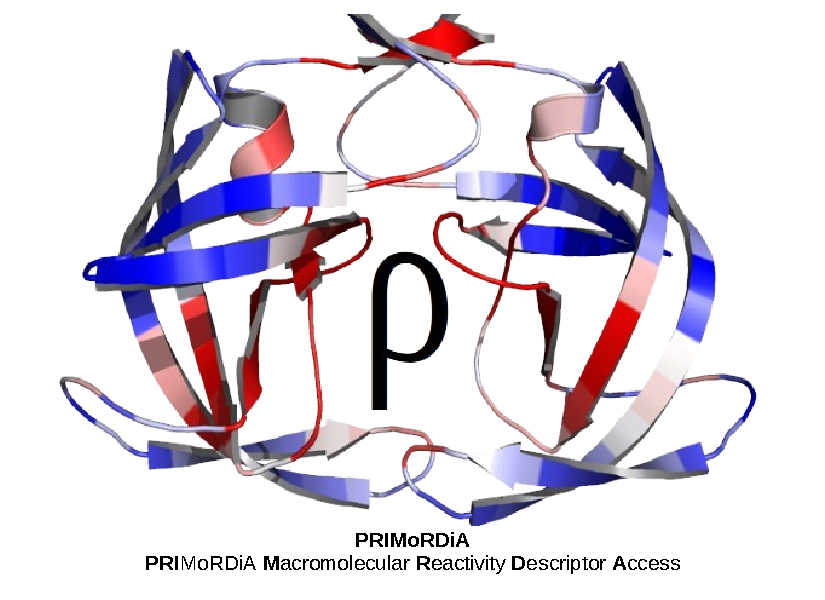
\includegraphics[width=7in]{images/logo_primordia}
\end{center}
\end{figure}	
\end{minipage}	
\newpage
			
\newpage
\tableofcontents
\newpage

\section*{Introdução}


Esse documento contém os tutoriais para o programa PRIMoRDiA. PRIMoRDiA ( \textbf{PRI}MoRDiA \textbf{M}acromolecular \textbf{R}eactivity \textbf{D}escriptors \textbf{A}ccess ) é um software escrito em \emph{C++}, desenvolvido para o pós-processamento eficiente dos resultados de pacotes de química computacional, produzindo uma grande variedade de descritores quânticos: propriedades eletrônicas e reatividade de sistemas químicos. 

O PRIMoRDiA traz implementado os principais descritores de reatividade da Teoria do DFT conceitual, incluindo as definições matemáticas para as teorias de elétrons de fronteira de Fukui e de ácidos e bases duros e moles de Pearson. O PRIMoRDiA foi desenvolvido com foco no cálculo de descritores e outras propriedades eletrônicas mais comuns para grandes moléculas que são relevantes para processos biológicos, e por isso há descritores modificados especificativamente para atender as particularidades desses sistemas. 

Também oferecemos um guia de usuário com informações gerais sobre a teoria e detalhes sobre o uso e interpretação dos resultados gerados pelo programa.  PRIMoRDiA foi desenvolvido na Universidade Federal da Paraíba, no Laboratório de Química Quântica e Computacional.

Para baixar os dados do repositório é possível usar o seguinte comando do git:

\hspace*{-\leftmarginwidth}
\begin{minipage}{\fullwidth}
	\begin{commandshell}git clone https://github.com/igorChem/PRIMoRDiA1.0v.git\end{commandshell}
\end{minipage}

Através desse comando, a pasta do repositório vai ser baixada no diretório de onde o seu terminal está aberto, podendo ser atualizado facilmente com o comando: 

\hspace*{-\leftmarginwidth}
\begin{minipage}{\fullwidth}
	\begin{commandshell}git pull\end{commandshell}
\end{minipage}

Também, no próprio site é possível baixar um '.zip' contendo todos os dados do repositório. 
No entanto, é fortemente recomentado que o usuário baixe uma das versões estáveis, de preferência a última. Essas versões estáveis tem a garantia de estarem com todas as suas funcionalidades devidamente testadas. 

\emph{\textbf{PRIMoRDiA é um programa que está em constante desenvolvimento e clonar o repositório em qualquer outro ponto que não seja as marcadas como estáveis pode gerar erros na utilização. }}

Link para última versão: \url{https://github.com/igorChem/PRIMoRDiA1.0v/releases/tag/v1.25}

Informações mais específicas sobre compilação, instalação e uso dos binários já compilados, consulte o guia de usuário fornecido no repositório. 

Sobre os tutoriais nesse documento, eles cobrem praticamente todas as funcionalidades do programa, mas sobretudo o que fazer com os resultados do PRIMoRDiA, já que a montagem do input e execução normalmente só necessitam de dois comandos em um terminal. O PRIMoRDiA trabalha com três modos de cálculo dos descritores, classificados pelo tipo de aproximação realizada. Os três primeiros tutoriais tratam exatamente desses três modos específicos de obter os descritores, tutoriais 4 e 6 trabalham aplicações em possíveis objetos de estudo e o tutorial 5 trabalha opções que não são executada através de input para gerar a densidade eletrônica e orbitais moleculares para sistemas quaisquer.

A lista de tutoriais está logo abaixo:

\begin{enumerate}
	\item Aproximação de Orbitais Congelados:
	\item Aproximação de Diferenças Finitas:
	\item Descritores de Banda
	\item Análise de Força Ácida
	\item Análise de Reação Enzimática
\end{enumerate}

O primeiro tutorial é muito importante de ser feito, pois ele introduz várias informações detalhadas sobre a montagem do input e execuções básicas no software gráfico Pymol para análise dos resultados de forma gráfica. Também, nesse mesmo tutorial, é desenvolvida a interpretação dos descritores globais e o efeito dos métodos de estrutura eletrônica nessas quantidades, informações que são relevantes para todos os métodos e modos de cálculo. 

O segundo tem pouca diferença no que diz respeito a montagem do input e execução do programa, e por isso aproveitamos para prover mais detalhes sobre o uso do Pymol. O terceiro é o principal tutorial para quem deseja trabalhar com macromoléculas, como proteínas/enzimas, introduzindo como utilizar os dois métodos implementados para o cálculo de descritores locais e outros vários parâmetros para a análise dos resultados.

O quarto tutorial pretende demonstrar o uso dos descritores dentro do contexto de uma pergunta de pesquisa, trazendo como exemplo a investigação da força ácida de diferentes amino-ácidos, mostrando como os diversos descritores podem ser utilizados e combinados para extrair informações de cálculos quânticos feitos para esses sistemas. 

O quinto tutorial traz uma aplicação bastante avançada do software, se assemelhando a análises que fazemos nas nossas recentes publicações. Os descritores de Banda, que são o terceiro tipo de modo de cálculo implementado exclusivamente no PRIMoRDiA para lidar com macromoléculas, aplicado a uma trajetória correspondendo a um caminho de reação de uma catálise enzimática. 

\newpage
\section{Tutorial 1: Aproximação de Orbitais Congelados}

Nesse tutorial vai ser demonstrado como utilizar o programa para obter os descritores de reatividade usando as informações dos orbitais moleculares de fronteira. Por ser o primeiro tutorial, vai ser exemplificado a obtenção dos descritores para a molécula de acroleína com a estrutura eletrônica calculada com os quatro pacotes de química computacional que é suportado pelo PRIMoRDiA.

\subsection{Contextualização}

As teorias de reatividade sempre foram muito mais exploradas dentro da química orgânica através do estudo de orbitais moleculares de fronteira, os famigerados HOMO e LUMO. Esse estudo compreende a análise da distribuição especial desses orbitais nas moléculas e seus valores de energia.

E por que esses orbitais são importantes? Primeiro, os orbitais moleculares servem para descrever a densidade de probabilidade de encontrar um elétron no espaço tridimensional; Segundo, durante as reações químicas são os elétrons que são transferidos entre as moléculas, reorganizando as ligações químicas e portanto as geometrias. Esses orbitais de fronteira, como HOMO (Highest Occupied Molecular Orbital) e LUMO (Lowest Unncupied Molecular Orbital), são os que descrevem a distribuição espacial do elétrons mais propensos a serem transferidos, ou dos níveis de energias virtuais mais propensos a receber elétrons.

Quando as teorias de reatividade foram demonstradas através do tratamento matemático baseado na Teoria de Densidade Funcional (DFT), os orbitais de fronteira se tornaram uma aproximação para funções locais e valores de energia para os descritores de reatividade. Essa é a aproximação de Orbitais Congelados, Frozen Ortbial Approximation (FOA) em inglês. Toda a parte teórica dessa aproximação, parte conceitual e derivação dos descritores de reatividade podem ser encontrados no nosso Guia do usuário e nas referências citadas lá. 

Essa aproximação tem algumas vantagens importantes, como necessitar de um protocolo de cálculo mais rápido que de diferenças finitas, e a consolidação dos conceitos baseados nos orbitais moleculares. A principal desvantagem é que por algumas vezes os orbitais HOMO e LUMO não são os que resultam na mais acura representação da reatividade do sistema.

Nesse tutorial, vamos mostrar como calcular os descritores de reatividade/quânticos usando FOA, como gerar e analisar os resultados usando software gráfico Pymol, analisando as tabelas com valores para cada átomo. Também, por ser o primeiro tutorial, vai ser dado mais atenção a detalhes técnicos sobre o input e scripts gerados pelo programa, interpretação de descritores e explicação de conceitos que serão úteis para os próximos tutoriais.

\subsection{Preparação dos Arquivos e Execução do Programa}

Basicamente, o que o PRIMoRDiA faz é extrair as propriedades eletrônicas de arquivos de saída (outputs) de pacotes de métodos de química quântica, e com essas informações fazer o tratamento matemático necessário para obter os descritores de reatividade. Esses descritores podem ser globais, representando uma propriedade que vale para todo o sistema molecular considerado no cálculo quântico, ou descritores locais, que por sua vez descrevem tanto uma propriedade para um dado ponto no espaço tridimensional quanto para cada átomo. 

Os descritores locais para os átomos são chamados de condensados, onde a parte do resultado da função local calculada para os descritores é atribuída para os átomos individualmente, tornando essa quantidade ligada as coordenadas do núcleo desse átomo.

Para exemplificar o funcionamento e uso do programa, a estrutura eletrônica da molécula de acroleína foi calculada nos quatro pacotes de química quântica que são suportados pelo PRIMoRDiA, GAMESS, MOPAC, ORCA e Gaussian, cada um com método de cálculo diferente. A representação gráfica do arranjo molecular da acroleína é mostrado logo abaixo.


\hspace*{-\leftmarginwidth}
\begin{minipage}{\fullwidth}
\begin{figure}[H]
\begin{center}
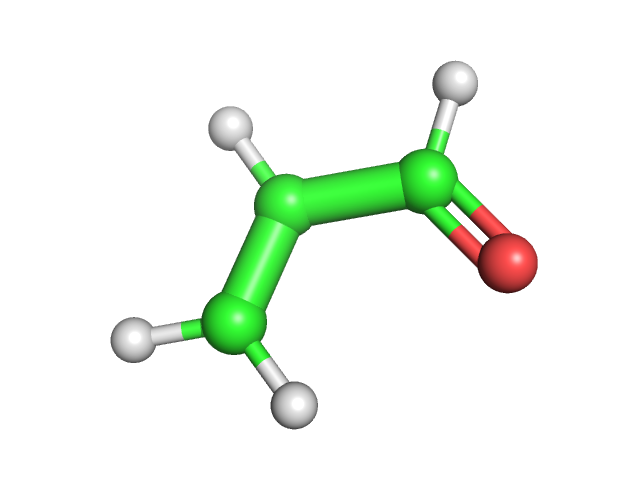
\includegraphics[width=3in]{images/img0}
\caption{Representação de esferas-e-bastões para a estrutura da molécula de acroleína.}
\label{fig_tut1_1}
\end{center}
\end{figure}
\end{minipage}	

Os arquivos que o PRIMoRDiA precisam estar na pasta comprimida Tutorials\_Files, que por sua vez tem as pastas para cada tutorial. Além desses arquivos, é necessário um arquivo de texto para indicar ao PRIMoRDiA o que fazer, famoso arquivo de input. Para gerar esse arquivo a partir dos arquivos de estrutura eletrônica que estão na pasta basta rodar o programa com a flag "-input" e os parâmetros específicos para o cálculo que se queira executar. Vamos executar o comando a baixo, dentro do diretório com os arquivos mencionados.

\hspace*{-\leftmarginwidth}
\begin{minipage}{\fullwidth}
\begin{commandshell}/path/to/PRIMoRDiA/PRIMoRDiA_1.25v_LINUX64 -input -op 1 -p mopac -grid 40\end{commandshell}
\end{minipage}

Nesse caso, o PRIMORDiA vai procurar na pasta os arquivos com a extensão ".aux", pois é requerido cálculos de descritores locais para arquivos de saída do mopac. Depois de executar esse comando vai aparecer no diretório dois arquivos novos: primordia.input e primordia.log. Se isso não ocorrer como descrito ou houver alguma mensagem de erro, verifique se o caminho para o executável está correto. Lembrando que é necessário trocar o "/path/to/primordia/" para o endereço da paste onde o executável está localizado. Abra o arquivo "primordia.input", o resultado deve ser como mostrado na seguinte caixa de texto ( \autoref{tut101} ).

\begin{minipage}{\textwidth}
\begin{lstlisting}[caption={Input gerado pelo comando do PRIMoRDiA.},label={tut101}]
#RT normal 
#PR eband 1 extrard pymols
1 acrolein.aux true 10 mopac 
\end{lstlisting}
\end{minipage}


Esse comando é útil para quando há vários arquivos para serem calculados na pasta. Vamos entender as opções utilizadas juntamente com a flag

\begin{itemize}
	\item \emph{-op}:\\ Indica a opção de cálculo que vai ser passada no próximo argumento.
	\item \emph{1}: \\ Opção de cálculo passada, ela indica que os descritores vão ser obtidos com FOA.
	\item \emph{-p}: \\Indica o programa de origem dos arquivos de saída.
	\item \emph{mopac}: \\É a keyword que indica que os arquivos de saída na pasta vieram do pacote de química quântica MOPAC.
	\item \emph{-grid}: \\ flag que serve para indicar a resolução da grade para os resultados dos descritores em representação volumétrica. Quanto maior o valor maior a resolução, mas também maior o custo computacional.
	\item \emph{40}: \\ Resolução da grade.
\end{itemize}

No entanto, há outros arquivos de saída na pasta oriundos de outros pacotes de química computacional, e para incluí-los é necessário edição manual do arquivo para que fique igual ao da seguinte caixa de texto (\autoref{tut102} ).

\begin{minipage}{\textwidth}
\begin{lstlisting}[caption={Input editado para execução do tutorial.},label={tut102}]
#RT normal 
#PR extrard pymols
1 acrolein.aux true 40 mopac 
1 acrolein_orca.out true 40 orca 
1 acrolein_gam.log true 40 gamess
1 acrolein_gauss.fchk true 40 gaussian 
\end{lstlisting}
\end{minipage}

A primeira linha do input sempre deve começar com \emph{"\#RT"}, que por padrão é seguido pela keyword \emph{"normal"}, que serve para indicar qual o Run Type ( tipo de cálculo ). Na segunda linha \emph{"\#PR"} indica que os próximos parâmetros vão ser para controlar aspectos gerais dos cálculos.

O parâmetro \emph{"pymols"} indica que queremos que o programa escreva scripts para automatizar a visualização dos resultados no Pymol. Todas as linhas no input que começarem com "\#" não vão ser consideradas, ou seja, é possível escrever comentários começando a linha dessa forma. As linhas que começarem com os inteiros, 1, 2 ou 3, serão consideradas para cálculo utilizando a opção correspondente.

Para executar o PRIMoRDiA é muito simples, a partir do nosso input criado e editado é só rodar o seguinte comando

\hspace*{-\leftmarginwidth}
\begin{minipage}{\fullwidth}
\begin{commandshell}/path/to/PRIMoRDiA/PRIMoRDiA_1.25v_LINUX64 -f primordia.input\end{commandshell}
\end{minipage}

A flag "-f" indica que o próximo argumento é um arquivo de input formatado para o programa. O arquivo de input pode ter qualquer nome e não é necessário que tenha a extensão ".input". Depois de rodar esse comando o programa deve indicar o tempo total de execução, e no mesmo diretório onde os dados e o input se encontram, vários novos arquivos de diferentes tipos devem aparecer. Vamos explicar eles a analisar na próxima parte do tutorial.


\subsection{Análises dos Resultados}

Os descritores de reatividade são calculados como quantidades globais, propriedades de todo o sistema, e locais, que é um mapeamento da reatividade sobre a topologia do sistema molecular. O PRIMoRDiA escreve arquivos com extensão ".GRD" para os descritores globais de cada entrada do sistema, e ".lrd" para os locais condensados e ".cube" para os locais volumétricos. Também escreve um arquivo com o final ".global", onde todos os descritores globais calculados são reunidos.

Se abrirmos esse arquivo, primordia.global, encontraremos dados como mostrado na \autoref{fig_tut1_2}. Esse arquivo já é formatado para ter o espaçamento ideal para ser copiado para um planilha, como mostrado na \autoref{fig_tut1_3}.


\hspace*{-1.2\leftmarginwidth}
\begin{minipage}{\fullwidth}
	\begin{figure}[H]
		\begin{center}
			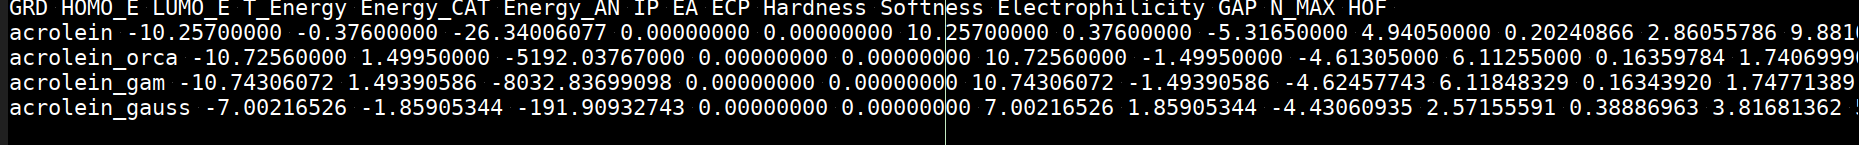
\includegraphics[width=7in]{images/img3}
			\caption{Resultados dos descritores globais para o input trabalhado nesse tutorial.}
			\label{fig_tut1_2}
		\end{center}
	\end{figure}
\end{minipage}	


\hspace*{-1.2\leftmarginwidth}
\begin{minipage}{\fullwidth}
	\begin{figure}[H]
		\begin{center}
			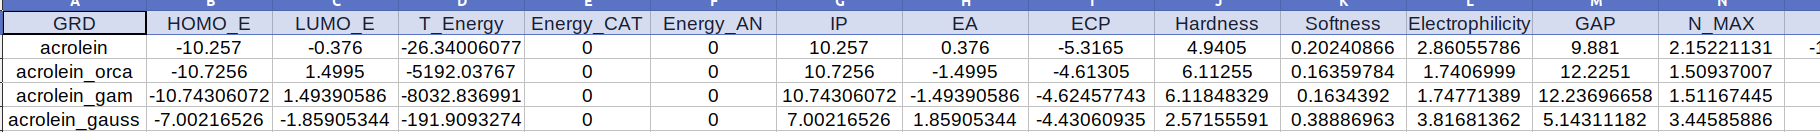
\includegraphics[width=7in]{images/img4}
			\caption{Resultados dos descritores globais transpostos para uma planilha.}
			\label{fig_tut1_3}
		\end{center}
	\end{figure}
\end{minipage}	

Para o Potencial de Ionização (IP), os valores ficaram em torno de 10 eV, com exceção dos resultados calculados a partir da saída GAUSSIAN, que utilizou o método DFT e apresentou 7 eV. Este valor é a energia necessária para extrair um elétron do sistema e é a base para outros descritores de reatividade junto com a afinidade eletrônica (EA), que é a mudança de energia quando o sistema recebe um elétron. 

O Potencial Químico Eletrônico (ECP) é o descritor do DFT conceitual que mede a propensão de um sistema molecular para doar elétrons, o que é muito semelhante entre os métodos de \textit{ab initio} e DFT usados aqui para a acroleína, mostrando a molécula mais propensa a doar elétrons quando os descritores provêm do cálculo semi-empírico.

O ECP frequentemente é um valor negativo que vem da derivada da energia eletrônica em relação ao número de elétrons, ou seja, os sistemas requerem energia para doar elétrons. Assim, interpretamos esses resultados como os menos negativos, pois requerem menos energia para doar elétrons e, assim, reagir por meio do processo de transferência de carga.

A dureza é a segunda derivada da energia eletrônica em relação ao número de elétrons e portanto a derivada do ECP em relação ao número de elétrons. Esses descritores indicam a resistência do sistema em doar elétrons, e um sistema com maior dureza é mais estável quimicamente. 

Os maiores valores de dureza calculados para a acroleína foram com os métodos Hartree-Fock e o menor com DFT. Assim, podemos concluir que o método DFT indicou a acroleína com maior propensão em doar seus elétrons e participar de uma reação química fazendo isso. A dureza sendo a derivada do ECP indica como ela mudará conforme a densidade de elétrons se move do sistema. Assim, um sistema pode ter um alto ECP, mas a alta dureza tornará a transferência da densidade do elétron mais difícil.

Energia de estabilização de um sistema para receber todos os elétrons possíveis é medida pela eletrofilicidade total. O número máximo correspondente de elétrons que o sistema pode receber é dado pelo descritor nMax e, finalmente, a diferença entre os orbitais moleculares da fronteira, HOMO e LUMO, 'gap' é o último descritor da lista. Para o método FOA, o gap e a dureza são a mesma quantidade, embora, para o método de aproximação por diferenças finitas isso não é verdade e as duas informações possam ser relevantes.


\subsubsection{Descritores Locais Condensados}

Agora, vamos analisar e interpretar os descritores locais, que são quantidades atribuídas a um ponto no espaço tridimensional. Existem duas maneiras comuns de representar os descritores locais para moléculas, que são implementadas no PRIMoRDiA. O primeiro é o condensado para átomos, onde os valores são atribuídos a cada átomo e são escritos como uma lista. Todas as entradas do arquivo de entrada produzem um '.lrd', especificamente para métodos FOA (opção 1 no arquivo de entrada), o sufixo do arquivo 'FOA.lrd'. Portanto, devemos ter quatro desses arquivos em nosso diretório, como podemos verificar usando o comando 'ls' no terminal Linux. Na imagem abaixo ( \autoref{fig_tut1_4} ), as informações desses arquivos foram transferidas para uma tabela do libreoffice calc.

\hspace*{-\leftmarginwidth}
\begin{minipage}{\fullwidth}
\begin{figure}[H]
\begin{center}
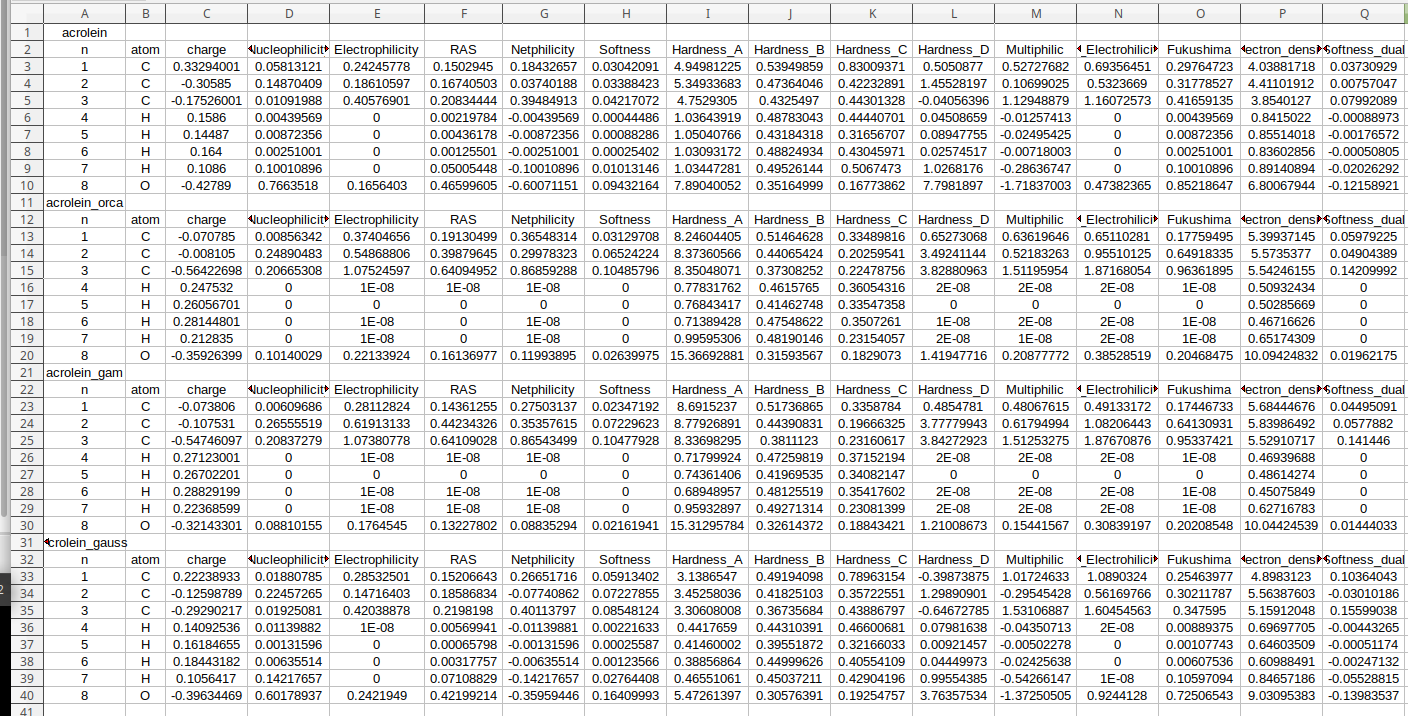
\includegraphics[width=6in]{images/img5}
\caption{Descritores locais condensados.}
\label{fig_tut1_4}
\end{center}
\end{figure}
\end{minipage}

Esses valores são mapeados para as coordenadas de cada núcleo atômico, conforme mostrado na figura acima( \autoref{fig_tut1_4} ), apresentando o oxigênio da acroleína como o mais reativo para receber um ataque eletrofílico.

Os átomos de carbono da dupla ligação também apresentam valores significativos de EAS. O valor mais alto de eletrofilicidade é do carbono 3. Este tipo de representação fornece um meio de comparação quantitativa, intermolecular e intramolecular. 

Na \autoref{fig_tut1_5}, mostramos os valores mapeados para os centros atômicos, para os descritores de eletrofilicidade e nucleofilicidade, calculados com os diferentes pacotes de química computacional e métodos de estrutura eletrônica. 

\hspace*{-\leftmarginwidth}
\begin{minipage}{\fullwidth}
\begin{figure}[H]
\begin{center}
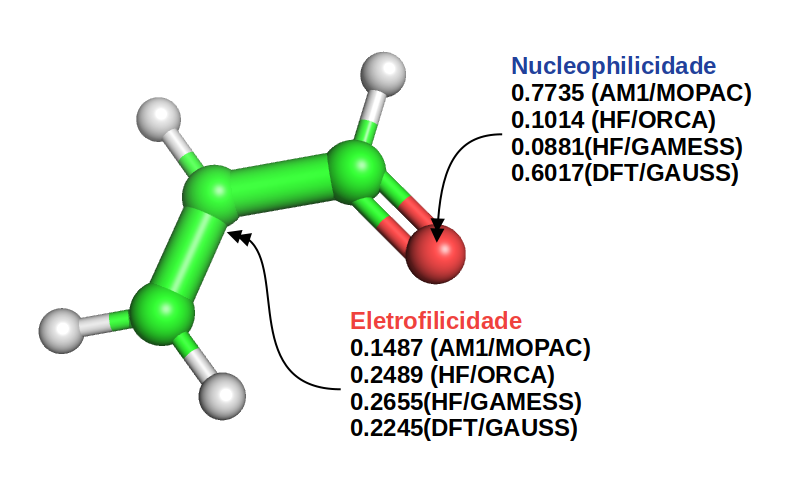
\includegraphics[width=4.5in]{images/img6}
\caption{Átomos mais reativos da molécula acroleína demonstrados pelos descritores.}
\label{fig_tut1_5}
\end{center}
\end{figure}
\end{minipage}


\subsubsection{Descritores Locais Volumétricos}

Para a representação volumétrica os arquivos Cubes gerados são utilizados para a renderização dos descritores no espaço tridimensional. Nas próximas imagens, mostraremos como gerar esta representação gráfica para os descritores de reatividade mais utilizados através do software Pymol. 

Você pode baixar Pymol do repositório (para Linux). Recomendamos fortemente que você faça os tutoriais básicos do Pymol, especialmente se desejar usá-lo para gerar suas figuras científicas, como fizemos várias vezes em nossas publicações. 

Os próximos passos consistem em gerar a renderização de volume em Pymol, um objeto que representa graficamente o campo escalar no espaço tridimensional, atribuindo a cada voxel de um mesmo valor a mesma cor e opacidade. A opacidade é um recurso importante, pois você precisa definir pelo menos dois níveis, cada um com uma cor diferente. Se esses dois ou mais níveis tiverem a mesma opacidade, apenas o mais próximo das bordas da grade aparecerá.

O PRIMoRDiA escreve scripts para automatizar a visualização desses arquivos no Pymol, vamos executar um deles para a acroleína calculada com semi-empírico. Abra o Pymol e digite o comando que está em destaque na figura abaixo ( \autoref{fig_tut1_6} ). 

\hspace*{-\leftmarginwidth}
\begin{minipage}{\fullwidth}
\begin{figure}[H]
\begin{center}
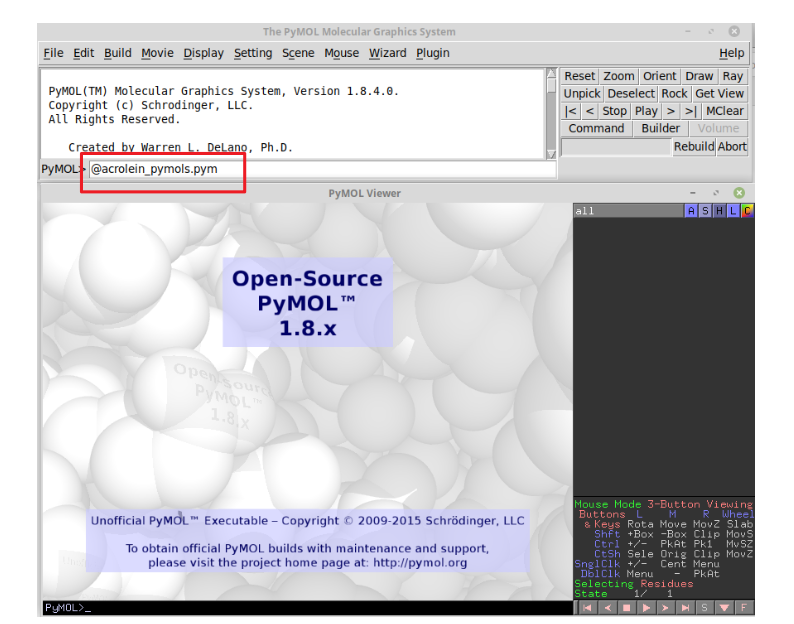
\includegraphics[width=4in]{images/img7}
\caption{Janela do Pymol e comando para executar dentro do programa para visualizar os descritores na representação volumétrica.}
\label{fig_tut1_6}
\end{center}
\end{figure}
\end{minipage}

O comando em destaque na caixa vermelha na \autoref{fig_tut1_6} está repetido abaixo

\hspace*{-\leftmarginwidth}
\begin{minipage}{\fullwidth}
	\begin{pymol}@acrolein_pymols.pym\end{pymol}
\end{minipage}

Depois da execução desse comando, todos os arquivos cube vão ser carregados, como mostrado na figura abaixo ( \autoref{fig_tut1_7} ). 

\hspace*{-\leftmarginwidth}
\begin{minipage}{\fullwidth}
\begin{figure}[H]
\begin{center}
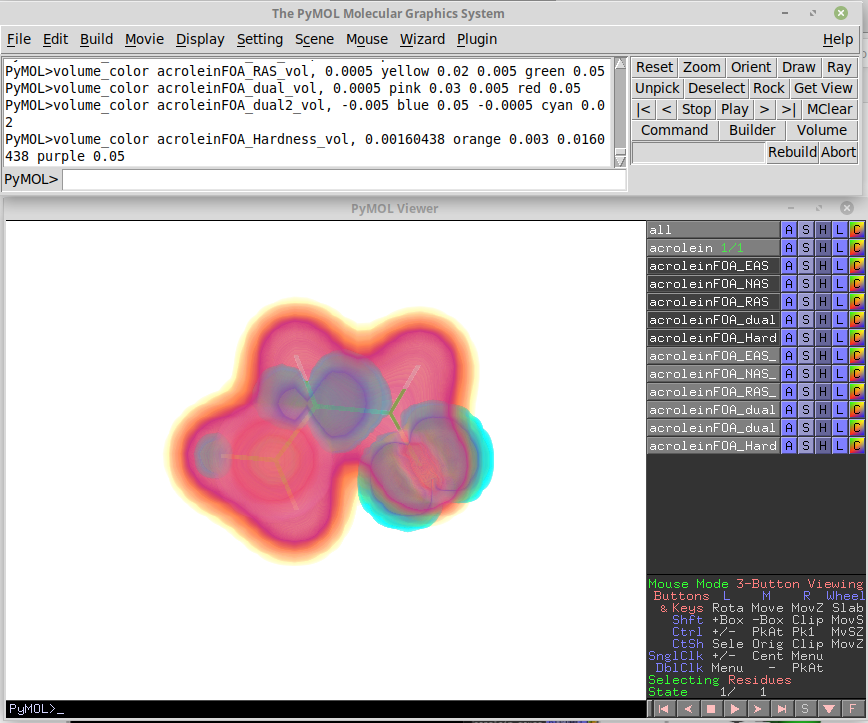
\includegraphics[width=4.5in]{images/img8}
\caption{Visualização dos descritores volumétricos gerada pelo script produzido pelo PRIMoRDiA.}
\label{fig_tut1_7}
\end{center}
\end{figure}
\end{minipage}

Selecionando o objeto acroleinFOA\_EAS\_vol na janela lateral do Pymol, mostraremos somente o descritor de nucleofilicidade. Usando o comando no Pymol


\hspace*{-\leftmarginwidth}
\begin{minipage}{\fullwidth}
	\begin{pymol}draw 1000,800,antialias=2\end{pymol}
\end{minipage}


Se renderiza uma imagem com resolução 1000X800 pixeis, e com parâmetro para aumentar a qualidade da imagem. seguido do comando de

\hspace*{-\leftmarginwidth}
\begin{minipage}{\fullwidth}
	\begin{pymol}png acrolein_eas.png\end{pymol}
\end{minipage}

salva a imagem em um arquivo em formato \textit{png} na pasta, como mostrada abaixo na ( \autoref{fig_tut1_8} )


\hspace*{-\leftmarginwidth}
\begin{minipage}{\fullwidth}
\begin{figure}[H]
\begin{center}
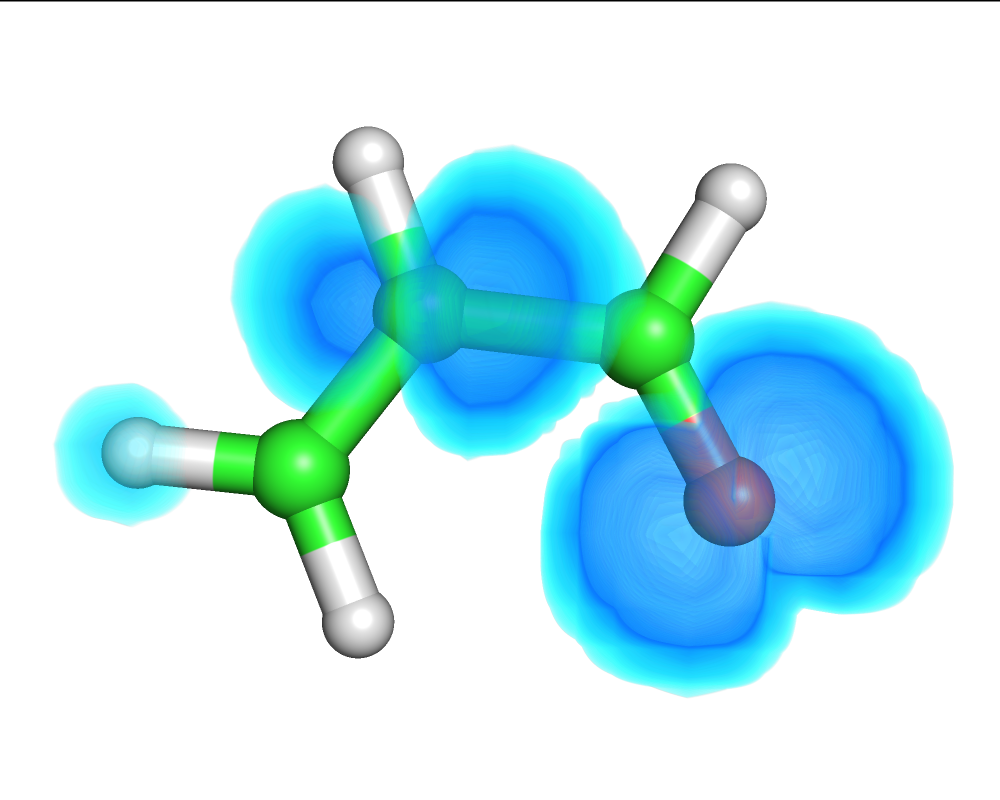
\includegraphics[width=3in]{images/img9}
\caption{Exemplo de imagem salva para o descritor de nucleofilicidade para a molécula de acroleína.}
\label{fig_tut1_8}
\end{center}
\end{figure}
\end{minipage}

O mesmo processo pode ser repetido para os outros objetos de volume. Também é possível usar a interface do Pymol para alterar os valores de superfície, cores e opacidades. Abaixo, a dureza local é objeto desse exemplo da \autoref{fig_tut1_9}.

E na \autoref{fig_tut1_10}, mostramos os descritores para a acroleína para todos os métodos de cálculo testados, mostrando os lugares suscetíveis da molécula para receber ataques eletrofílicos (azul) e nucleofílicos (rosa).

\hspace*{-\leftmarginwidth}
\begin{minipage}{\fullwidth}
\begin{figure}[H]
\begin{center}
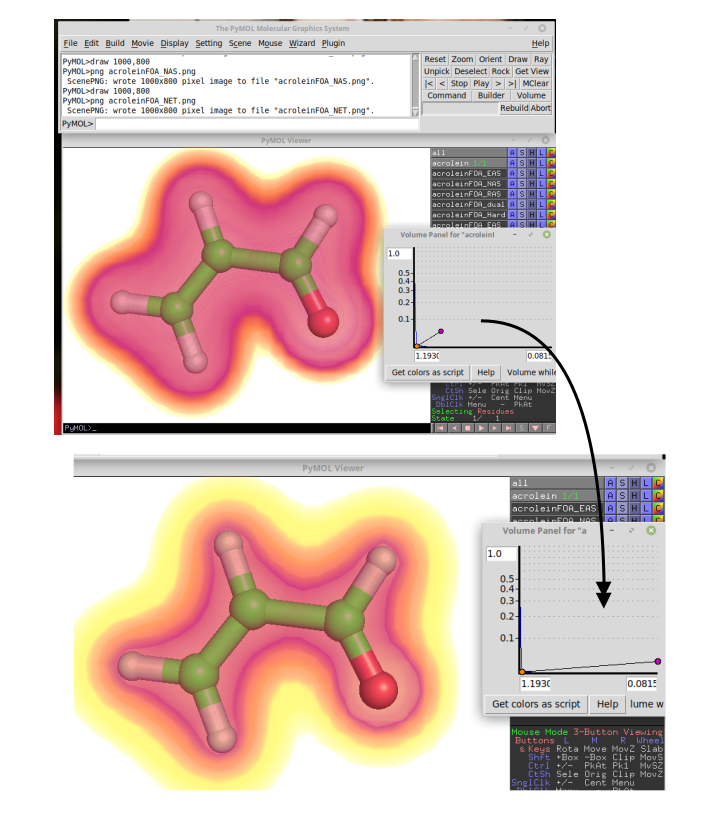
\includegraphics[width=4in]{images/img10}
\caption{Renderização do descritor de dureza local.}
\label{fig_tut1_9}
\end{center}
\end{figure}
\end{minipage}

\hspace*{-\leftmarginwidth}
\begin{minipage}{\fullwidth}
\begin{figure}[H]
\begin{center}
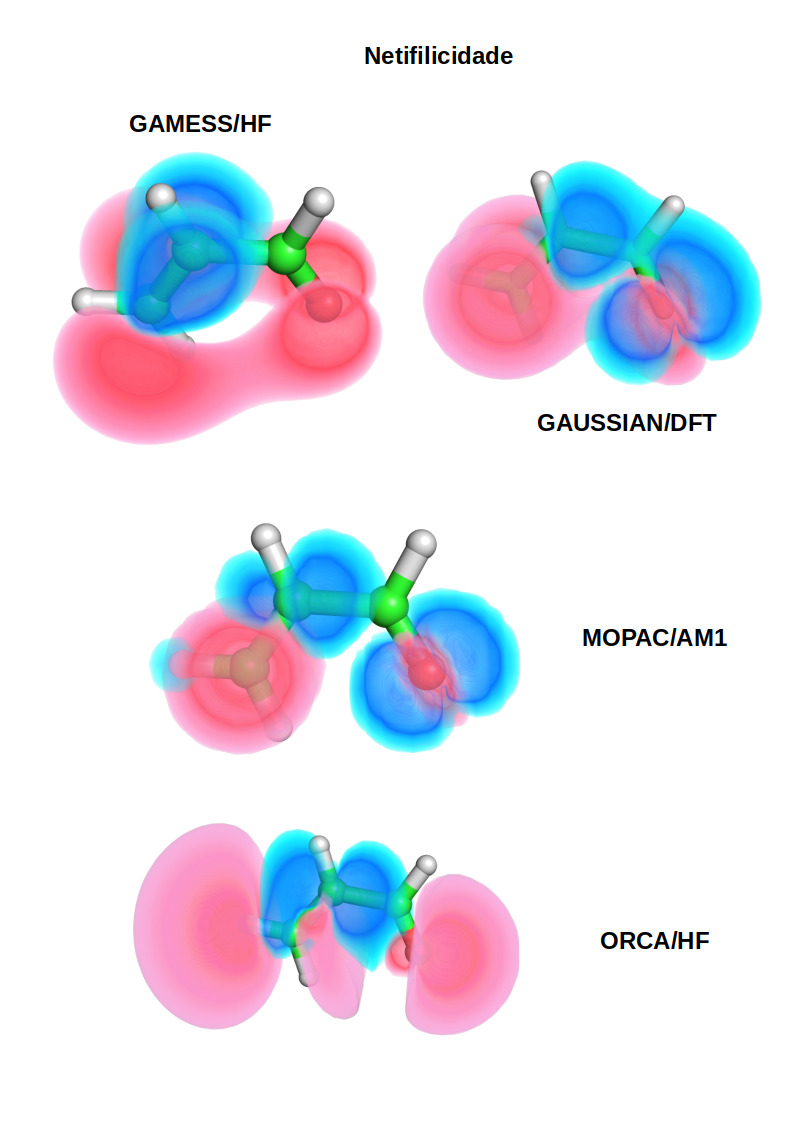
\includegraphics[width=4in]{images/img11}
\caption{Descritor de Netfilicidade para a acroleína usando diferentes métodos de estrutura eletrônica trabalhados nesse tutorial.}
\label{fig_tut1_10}
\end{center}
\end{figure}
\end{minipage}

Portanto, nesse tutorial podemos ver também a influência dos métodos de estrutura eletrônica na obtenção dos descritores, que é significativa mas tende a ser bem menor que o efeito provocado nos resultados energéticos, podendo, na maioria das vezes, que os descritores sejam obtidos com métodos menos custosos. 

\newpage
\section{Tutorial 2: Aproximação de Diferenças Finitas}

Esse segundo tutorial demonstra o cálculo dos descritores no PRIMoRDiA com a aproximação de diferenças finitas, usando a molécula de benzeno como sistema modelo.  

Há pouca diferença entre esse tutorial e o primeiro na parte de execução de comandos e ferramentas de análise de resultados. Sobre o que é necessário para o cálculo, o método de diferenças finitas requer dois arquivos extras de estrutura eletrônica, para os estados carregados positivamente e negativamente em relação ao estado eletrônico que se queira calcular as propriedades. 


\subsection{Contextualização}

Em geral, o método de diferenças finitas é uma ferramenta amplamente utilizada para o cálculo de derivadas de forma numérica, ou seja, substituindo um método analítico. Nesse caso mais específico, o cálculo dessas propriedades eletrônicas definidas como derivadas em relação ao número de elétrons, o método de diferenças finitas é um caminho quase intuitivo, já que não é possível derivar uma função não continua. 

Por isso o método de diferenças finitas é uma forma tradicional de calcular os descritores e é implementado no PRIMoRDiA extensivamente. Também, devido ao fato de calcular as propriedades utilizando a informação da diferença das densidades eletrônicas completas, os descritores locais calculados por esse método tendem a ser mais acurados em respeito a efeitos dos orbitais moleculares que não só o HOMO e LUMO. No entanto, a necessidade de dois single points a mais e a obtenção da densidade eletrônica total faz com que esse método acabe se tornando computacionalmente mais custoso. 

Nesse tutorial vamos usar a molécula de benzeno como exemplo para os descritores com esse método de aproximação. A molécula de benzeno não é apresenta pontos de reatividade específicos devido a sua simetria, mas é possível visualizar propriedades relacionadas com aromaticidade e a geometria do anel. 

\subsection{Preparação dos Arquivos e Execução do Programa}

Todos os arquivos necessários para realizar o tutorial estão no repositório junto ao código, no arquivo comprimido de nome Tutorials\_Files. Nesse exemplo vamos utilizar a estrutura eletrônica para a molécula de benzeno em três estados de carga, calculados com o método semi-empírico AM1 no pacote de química computacional MOPAC. Observe que no input para execução desse tutorial, mostrado na caixa de texto \autoref{tut201}, os nomes dos arquivos de saída do MOPAC tem a extensão ".out". 

\hspace*{-\leftmarginwidth}
\begin{minipage}{\fullwidth}
\begin{lstlisting}[caption={Input editado para execução do tutorial 2},label={tut201}]
#RT normal
#PR pymols extrard
2 benzene.out benzene_cat.out  benzene_an.out true 30 1 mopac
\end{lstlisting}
\end{minipage}

Esses arquivos não contém a estrutura eletrônica completa para os sistemas, no entanto o PRIMoRDiA entende que na mesma pasta que esses arquivos estejam também os correspondes com a extensão ".mgf". Esses arquivos possuem as matrizes necessárias para operações de álgebra linear para obter corretamente a densidade eletrônica total com os dados que saem do MOPAC. 

Para grandes moléculas, o MOPAC não consegue gerar esse arquivo, já que ele é muito cara de se escrever para estruturas com muitos átomos. Nesse caso o cálculo de diferenças finitas tem que ser feito usando os arquivos do tipo ".aux", que a partir deles o PRIMoRDiA gera uma densidade eletrônica total baseada nos orbitais moleculares, mas não garante a sua integração exata para o número de elétrons do sistema. 

O cálculo dos descritores usando diferenças finitas para grandes moléculas é de fato um tanto incomum, devido ao custo computacional de se obter três estruturas eletrônicas e os cálculos de densidade total para toda a extensão do sistema. Entretanto, com as modificações apropriadas dos descritores usando a aproximação de Orbitais Congelados, FOA, não é necessário recorrer a diferenças finitas para estudar proteínas, fragmentos de DNA e/ou outras moléculas relevantes aos processos biológicos.  

Indo para a execução do PRIMoRDiA em si, é bem simples e direto, uma vez com o input e os arquivos necessários na pasta basta rodar o seguinte comando no seu terminal


\hspace*{-\leftmarginwidth}
\begin{minipage}{\fullwidth}
	\begin{commandshell}/path/to/PRIMoRDiA/PRIMoRDiA_1.25v_LINUX64 -f primordia.input\end{commandshell}
\end{minipage}

Exatamente da mesma forma como foi mostrada no tutorial anterior. Depois da execução desse comando, o programa deve finalizar sem nenhum erro e gerar diversos arquivos com os resultados na paste onde o programa rodou. 

\subsection{Análises dos Resultados}

Como no tutorial anterior, nos vamos abrir os arquivos contendo o resumo dos descritores globais e locais, e finalizar a análise visualizando os descritores locais volumétricos usando o software Pymol. 

Na \autoref{fig_tut2_1}, mostramos o arquivo benzene\_FD.GRD aberto em um editor de texto, mostrando os valores obtidos para os descritores globais e outras propriedades eletrônicas que são extraídas pelo PRIMoRDiA. A grande diferença para o primeiro tutorial é a presença dos valores de energia eletrônica para os estados catiônico e aniônico. Além disso, o valor de \emph{gap} aqui, continua sendo a diferença de energia do HOMO e LUMO para a estrutura eletrônica do estado de carga neutro, ou seja, as informações em relação a potencial de ionização e afinidade eletrônica não são redundantes nesse caso.  

\hspace*{-\leftmarginwidth}
\begin{minipage}{\fullwidth}
	\begin{figure}[H]
		\begin{center}
			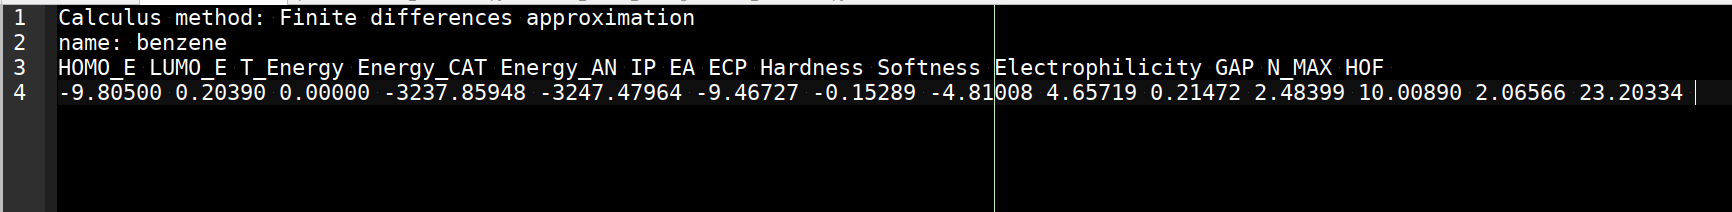
\includegraphics[width=7in]{images/tut2_img2}
			\caption{Arquivo de saída do PRIMoRDiA para os descritores globais calculados para a molécula de Benzeno com o método de diferenças finitas.}
			\label{fig_tut2_1}
		\end{center}
	\end{figure}
\end{minipage}

Avançando para a análise dos descritores locais condensados, o arquivo "benzeneFD.lrd" é mostrado na \autoref{fig_tut2_2} aberto em um editor de texto. Como já vimos antes, esse arquivo é formatado de forma a ser facilmente copiado e colado em um software de planilhas, como mostrado na \autoref{fig_tut2_3}.

\hspace*{-\leftmarginwidth}
\begin{minipage}{\fullwidth}
	\begin{figure}[H]
		\begin{center}
			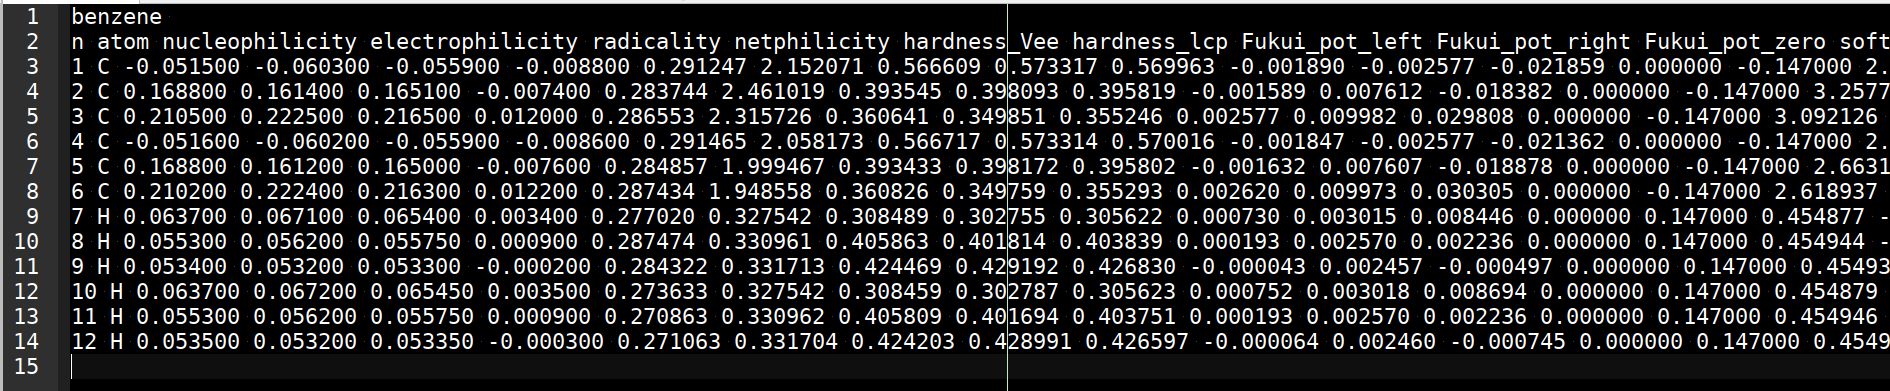
\includegraphics[width=7in]{images/tut2_img3}
			\caption{Arquivo de saída do PRIMoRDiA para os descritores locais condensados para os átomos da molécula de benzeno, obtidos com o método de diferenças finitas.}
			\label{fig_tut2_2}
		\end{center}
	\end{figure}
\end{minipage}

\hspace*{-1.2\leftmarginwidth}
\begin{minipage}{\fullwidth}
	\begin{figure}[H]
		\begin{center}
			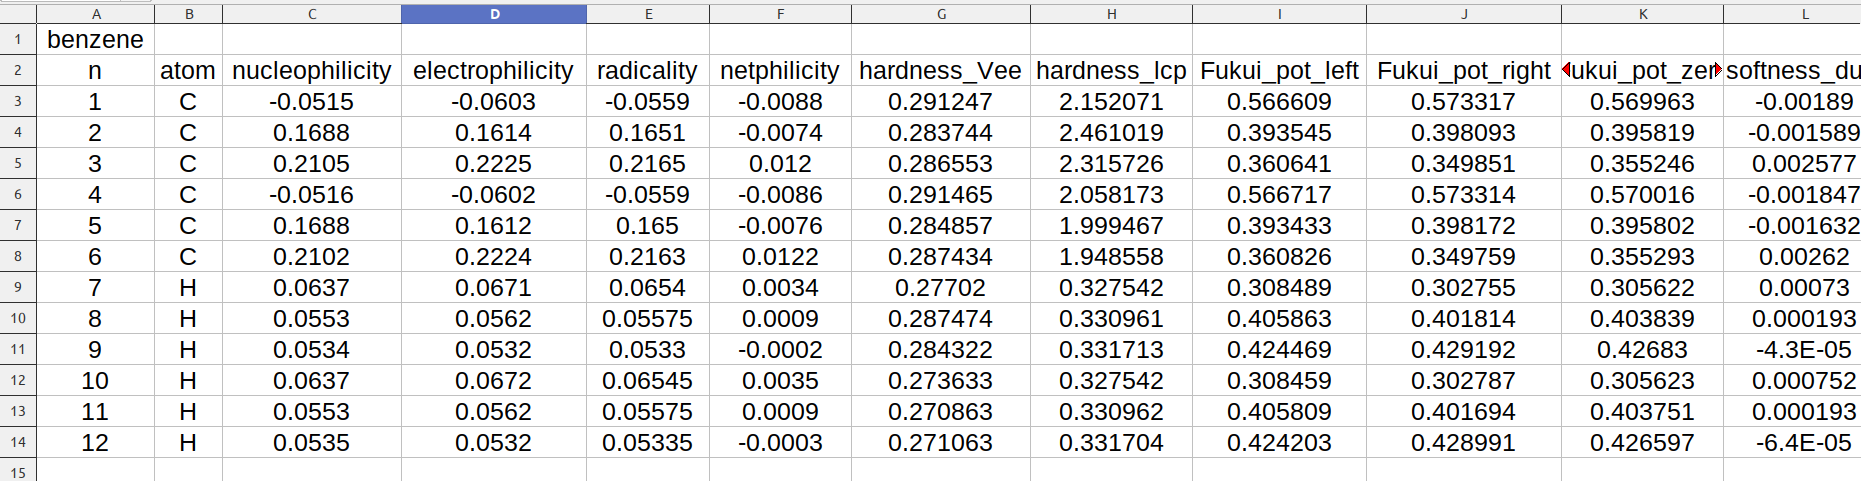
\includegraphics[width=7in]{images/tut2_img4}
			\caption{Planinha eletrônica com os dados dos descritores locais condensados para os átomos da molécula de benzeno obtidos com o método de diferenças finitas.}
			\label{fig_tut2_3}
		\end{center}
	\end{figure}
\end{minipage}

Nós podemos observar a partir dos dados dispostos na \autoref{fig_tut2_3}, os diversos descritores locais obtidos com o cálculo do PRIMoRDiA, assim como propriedades extraídas do arquivo de saída dos programas de química computacional, como nesse caso a coluna de \emph{charge}, mostrando as cargas parciais para os átomos do sistema de referência. O descritor chamado de \emph{Fukushima} é a localização dos orbitais de fronteira em cada átomo, e portanto não é alterado pelo métodos de diferenças finitas. 

Observando os descritores de nucleofilicidade e eletrofilicidade, podemos perceber que há valores negativos associados a alguns átomos. Quando esses valores são de pequena grandeza comparados com os átomos mais reativos não há o que se preocupar quanto a qualidade dos cálculos, pois é uma característica do método de diferenças finitas indicar regiões onde a densidade eletrônica diminui frente a um processo de ganho de carga e, ou aumenta frente a um processo de perda de carga. Essas variações podem ocorrer, desde que pequenas, e devem ser interpretadas com cuidado dentro do contexto do processo modelado. 

Ainda sobre esses dois descritores, podemos ver que os átomos que apresentam alta nucleofilicidade também apresentam alta eletrofilicidade. Por ser simétrico, o benzeno tende a apresentar padrões de reatividade bem distribuídos nos átomos de carbono e geralmente guiados pela geometria do anel. Portanto a análise desses descritores numéricos por átomo pode acabar se tornando confusa para esse tipo de sistemas, e por isso é mais interessante avaliar os descritores locais na representação volumétrica. 

Assim como em todos os tutoriais nesse documento, nós vamos utilizar o software gráfico Pymol, se aproveitando do script escrito pelo PRIMoRDiA, que na pasta deve ter o nome de \emph{benzene\_pymols.pym}, que pode ser visualizado aberto em editor de texto na \autoref{fig_tut2_4}. 

\hspace*{-\leftmarginwidth}
\begin{minipage}{\fullwidth}
	\begin{figure}[H]
		\begin{center}
			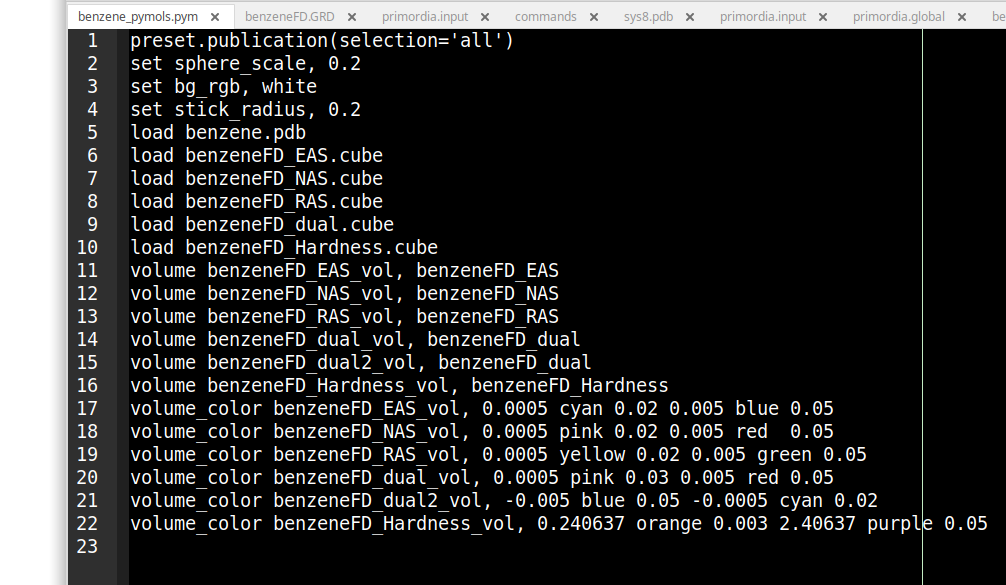
\includegraphics[width=4.5in]{images/tut2_img5}
			\caption{Editor de texto com o arquivo de script escrito pelo PRIMoRDiA para automatizar a visualização dos descritores volumétricos no Pymol.}
			\label{fig_tut2_4}
		\end{center}
	\end{figure}
\end{minipage}

Através de seu terminal, com o caminho correspondente ao diretório/pasta dos arquivos do tutorial, abra a janela do Pymol, e no seu terminal execute o seguinte comando 

\hspace*{-\leftmarginwidth}
\begin{minipage}{\fullwidth}
	\begin{pymol}@benzene_pymols.pym\end{pymol}
\end{minipage}
 
A partir desse comando, o Pymol vai carregar os arquivos .cube e um de PDB também gerado pelo PRIMoRDiA, todos de uma vez. A janela de ficar como a mostrada na \autoref{tut2_img6}.

\hspace*{-\leftmarginwidth}
\begin{minipage}{\fullwidth}
	\begin{figure}[H]
		\begin{center}
			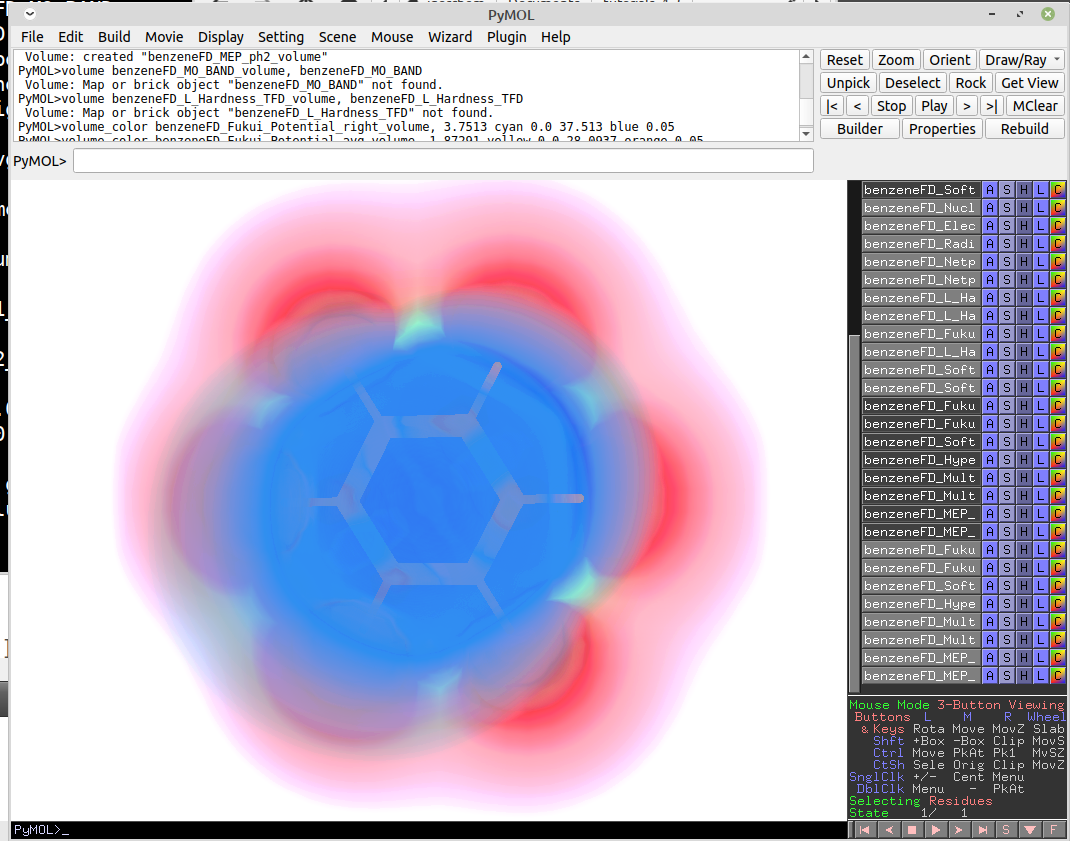
\includegraphics[width=4in]{images/tut2_img7}
			\caption{Software Pymol com os dados do tutorial carregados a partir do script gerado no PRIMoRDiA.}
			\label{fig_tut2_6}
		\end{center}
	\end{figure}
\end{minipage}

Na parte lateral da janela estão listados os objetos carregados, e os que estão mais iluminados são aqueles que estão ativos e aparacendo na tela. Selecione somente um e para salvar a imagem dessa representação em alta resolução execute o seguinte comando 

\hspace*{-\leftmarginwidth}
\begin{minipage}{\fullwidth}
	\begin{pymol}draw 3000,2800,antialias=2\end{pymol}
\end{minipage}

Depois de alguns segundos, ou minutos dependendo do poder computacional e de placas gráficas disponíveis, essa imagem aparece em destaque em um fundo preto, como na \autoref{tut2_img8}. 
A imagem foi renderizada, para salva-lá definitivamente no disco, use o seguinte comando

\hspace*{-\leftmarginwidth}
\begin{minipage}{\fullwidth}
	\begin{pymol}png benzene_nuc.png\end{pymol}
\end{minipage}

\hspace*{-\leftmarginwidth}
\begin{minipage}{\fullwidth}
	\begin{figure}[H]
		\begin{center}
			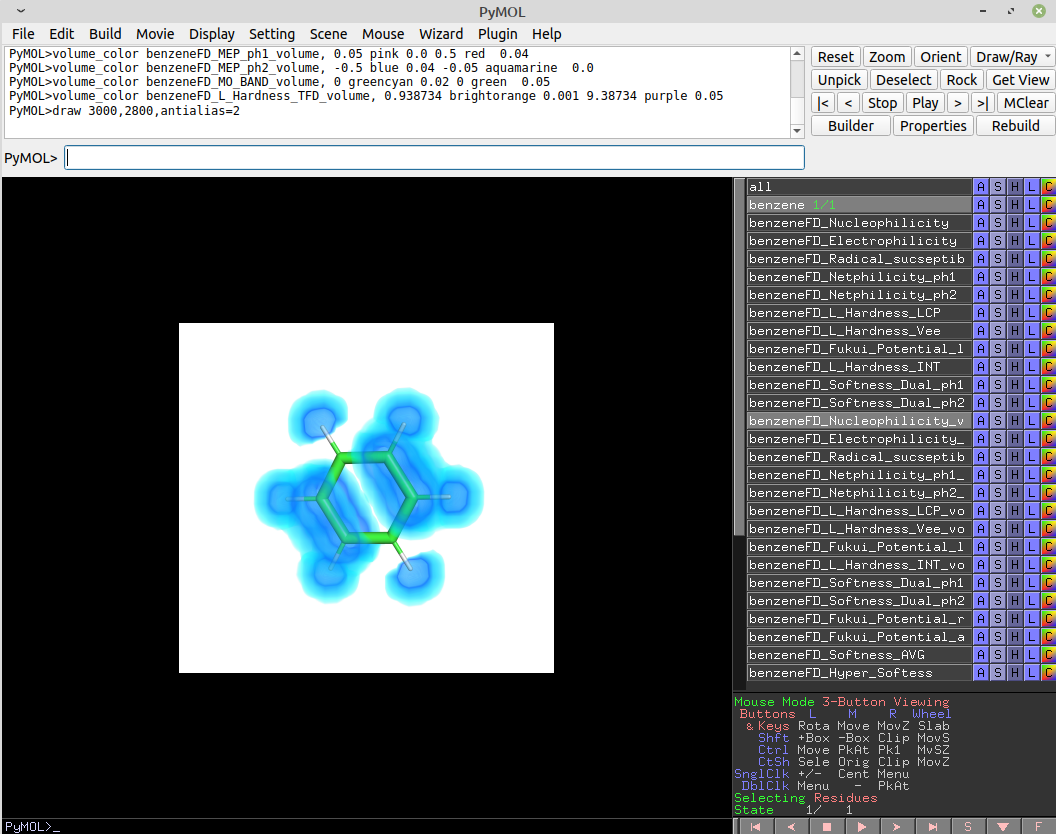
\includegraphics[width=4in]{images/tut2_img8}
			\caption{Imagem do descritor volumétrico de nucleofilicidade renderizada no software Pymol.}
			\label{fig_tut2_7}
		\end{center}
	\end{figure}
\end{minipage}

Podemos notar que esse descritor apresenta uma distribuição bem simétrica para todo a molécula, mas não seguindo o padrão circular, dando preferência a quatro átomos de carbono  do anel em detrimento dos outros dois. 

Um descritor interessante de se observar é o de dureza química local, que no PRIMoRDiA pode ser obtido com até sete diferentes equações de trabalho, que são completamente explicadas no guia do usuário. O PRIMoRDiA não coloca no script todos os descritores locais possíveis, até para não sobrecarregar o software gráfico, pois dependendo dos recursos computacionais disponíveis o mesmo pode travar. 

Também, para todos os descritores, o PRIMoRDiA sugere uma paleta de cores, então geralmente não há necessidade de ajustar manualmente os valores e opacidades das iso-superficies, como já foi mostrado em tutoriais antigos. De qualquer forma, é indicada que os tutoriais do Pymol sejam realizados para a produção de imagens mais customizadas. 

Voltando para os descritores de dureza local, na \autoref{fig_tut2_8} nos mostramos a renderização desse descritor calculado com a equação de trabalho que se baseia na aproximação do potencial químico local, abreviada de LCP. Já na figura \autoref{fig_tut2_9}, é mostrada a dureza local estimada com a aproximação da parte de interação inter-eletrônica do potencial eletrostático molecular. Outra propriedade local que representa as interações de tipo duro-duro, aquelas controladas-por-carga como explicado no guia do usuário, é o próprio potencial eletrostático molecular mostrado na \autoref{fig_tut2_10}. 

\hspace*{-\leftmarginwidth}
\begin{minipage}{\fullwidth}
	\begin{figure}[H]
		\begin{center}
			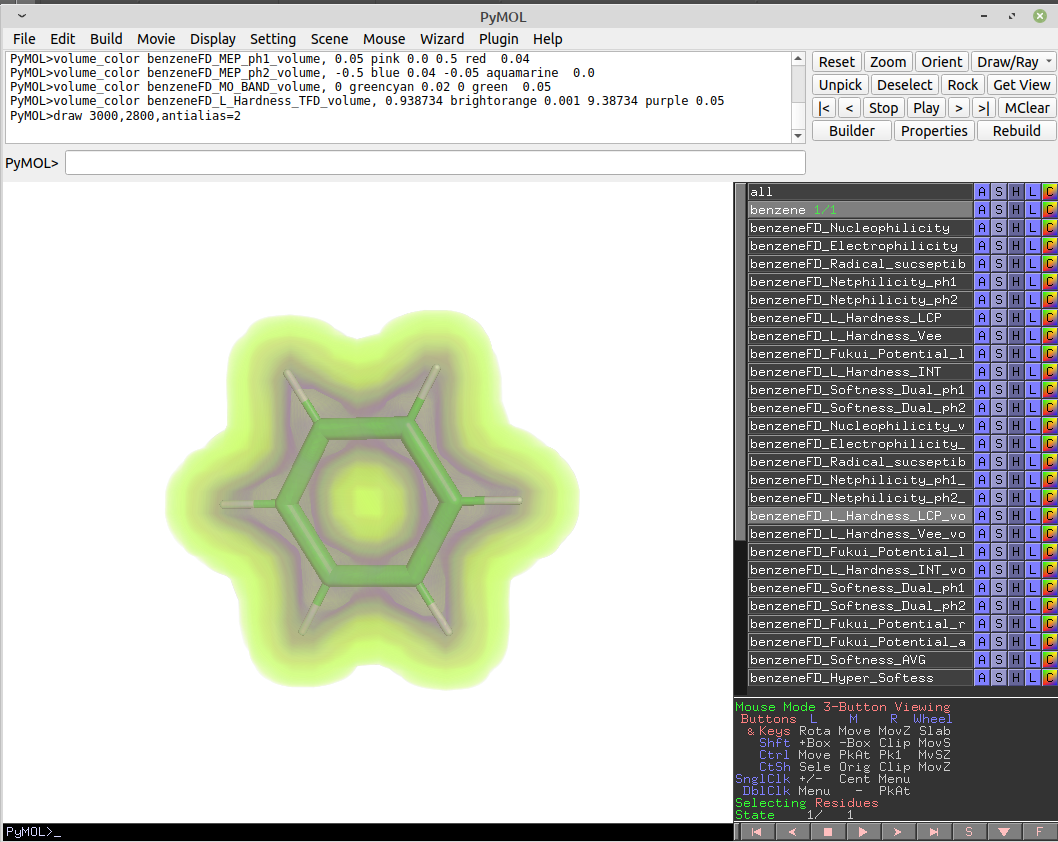
\includegraphics[width=4in]{images/tut2_img9}
			\caption{Dureza local usando, a aproximação de potencial químico local, renderizada no Pymol.}
			\label{fig_tut2_8}
		\end{center}
	\end{figure}
\end{minipage}

\hspace*{-\leftmarginwidth}
\begin{minipage}{\fullwidth}
	\begin{figure}[H]
		\begin{center}
			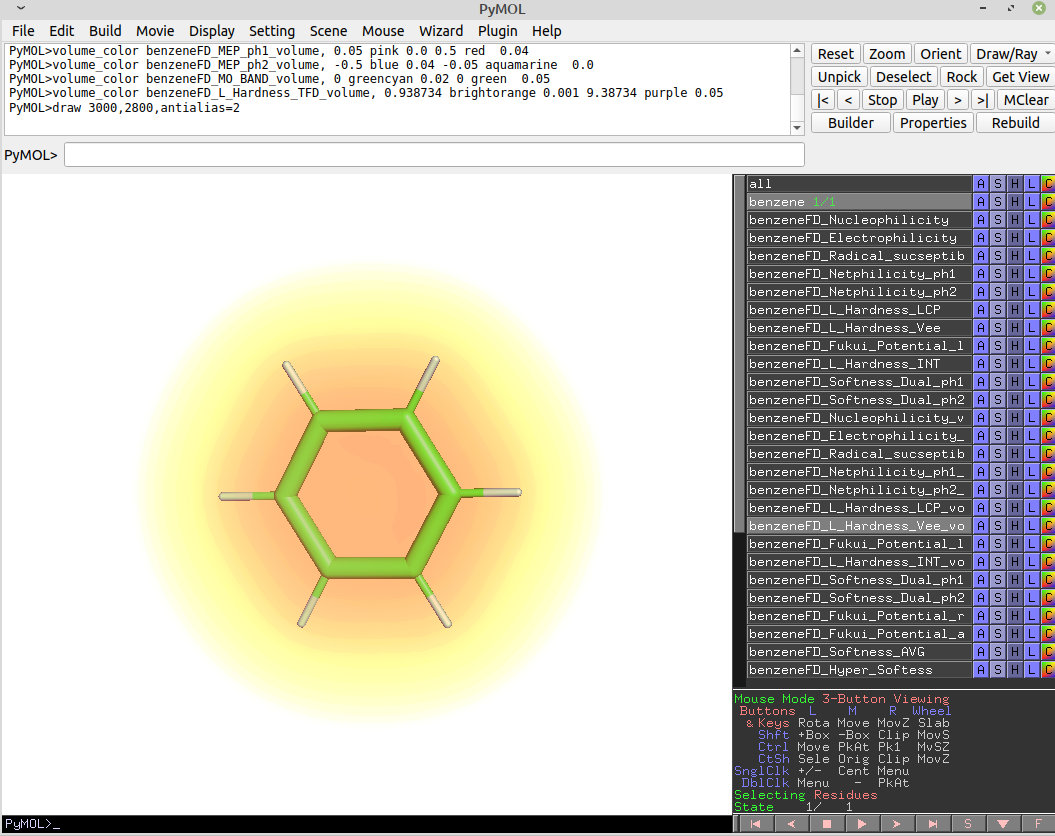
\includegraphics[width=4in]{images/tut2_img10}
			\caption{Dureza local usando, a aproximação de interação inter-eletrônica do potencial eletrostático molecular, renderizada no Pymol.}
			\label{fig_tut2_9}
		\end{center}
	\end{figure}
\end{minipage}


\hspace*{-\leftmarginwidth}
\begin{minipage}{\fullwidth}
	\begin{figure}[H]
		\begin{center}
			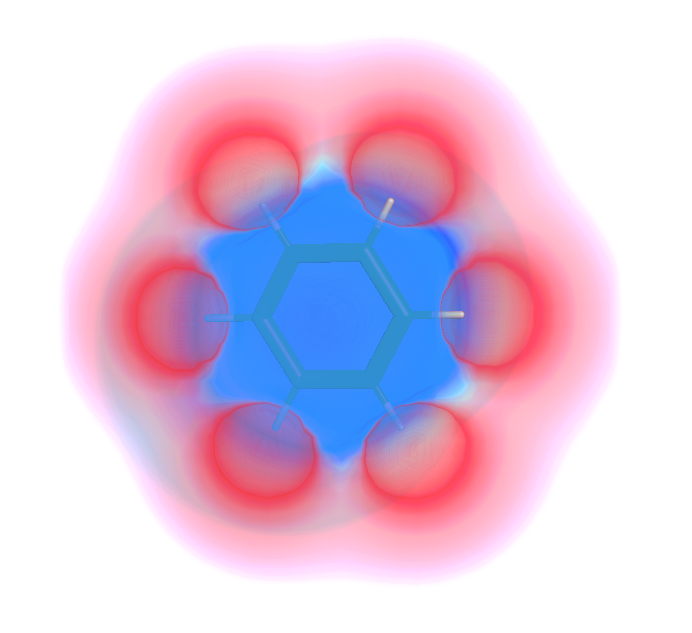
\includegraphics[width=3.3in]{images/tut2_img12}
			\caption{Potencial eletrostático molecular estimado a partir da cargas parciais. Imagem renderizada e salva em png.}
			\label{fig_tut2_11}
		\end{center}
	\end{figure}
\end{minipage}

A partir desses descritores, podemos ver como as principais interações com a densidade eletrônica surgem a partir do centro do anel aromático. 

\newpage
\section{Tutorial 3: Descritores de Banda}

Assim como na aproximação de orbitais congelados, nesse tutorial vamos explorar dois métodos de combinação de orbitais de fronteira para o ajuste desses descritores para macromoléculas. Para os cálculos, vamos utilizar um polipeptídeo bastante comum em testes, a TRP-cage, que teve a estrutura eletrônica obtida usando métodos semiempiricos implementados no MOPAC, incluindo o método de escalonamento linear MOZYME.

Assuntos abordados nesse tutorial:

\begin{itemize}
	\item Cálculo dos descritores usando nossos métodos de banda dos orbitais de fronteira.
	\item Uso do pacote gráfico Pymol para visualização e geração de imagens de alta qualidade para os descritores condensados. 
	\item Demonstração dos descritores condensados por resíduos
	\item Representação volumétrica para esses descritores, em especial para regiões limitadas definidas pelo usuário
	\item Análise de densidade de estados de energia
\end{itemize}

\subsection{Contextualização}

O PRIMoRDiA é um programa que foi desenvolvido desde o início para o cálculo de descritores de reatividade para grandes moléculas com relevância para sistemas biológicos, mais especificamente proteínas e fragmentos de DNA/RNA. Essas moléculas são biopolímeros e possuem uma estrutura eletrônica peculiar, com vários orbitais moleculares com energias similares as do HOMO e LUMO e com distribuição espacial relevante para processos químicos que envolvam esses sistemas.

\subsection{Preparação dos Arquivos e Execução do Programa}

Os arquivos necessários para realizar o tutorial estão na pasta comprimida Tutorials\_Files deste repositório. Os arquivos correspondem a outputs programa mopac de cálculos feitos com método semi-empírico PM7, um com método de escalonamento linear mozyme 2jof\_PM7\_lmo.aux, e sem esse método 2jof\_PM7.aux. Para cada um desses arquivos tem um arquivo de PDB, que contém as informações relevantes ao biopolímero que vai ser utilizado pelo PRIMoRDiA para escrever descritores e representações especiais. Esses PDBs são baseados no que pode ser encontrado pelo código 2JOF. A representação em cartoon desse polipeptídeo se encontra abaixo na \autoref{fig_tut3_1}.


\hspace*{-\leftmarginwidth}
\begin{minipage}{\fullwidth}
	\begin{figure}[H]
		\begin{center}
			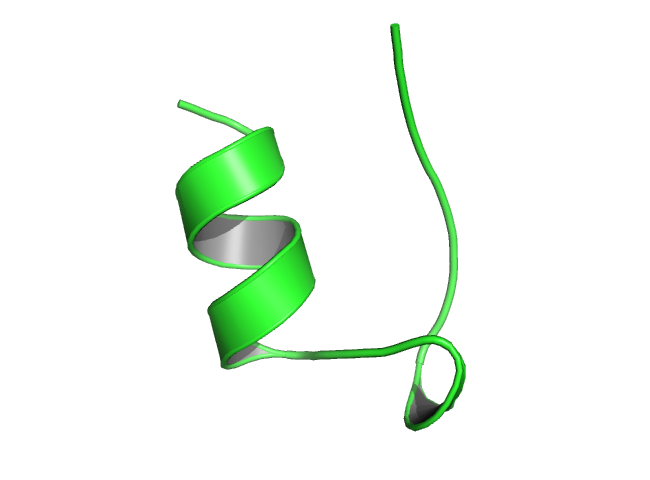
\includegraphics[width=4in]{images/tut3_img1}
			\caption{Representação cartoon para o polipeptídeo TRP-cage.}
			\label{fig_tut3_1}
		\end{center}
	\end{figure}
\end{minipage}

Para facilitar a produção de input a partir desses arquivos vamos usar o seguinte comando


\hspace*{-1.2\leftmarginwidth}
\begin{minipage}{\fullwidth}
\begin{commandshell}path/to/PRIMoRDiA_1.25v_LINUX64 -input -op 3 -p mopac\end{commandshell}
\end{minipage}


Um arquivo de chamado de primordia.input é gerado na pasta, igual ao mostrado na \autoref{tut303}. A primeira keyword encontrada no arquivo é "\#RT normal" para indicar que o Run Type ( tipo de cálculo ) é do tipo comum esperado para a execução do PRIMoRDiA. O keyword "\#PR" indica os que as próximas entradas na linha são parâmetros especiais, que no caso, por hora, é "eband" e "1", indicando que o limite para considerar orbitais moleculares em relação HOMO-LUMO é de 1eV. As duas linhas que começam com o inteiro "3", indicam a opção de cálculo do PRIMoRDiA especial para macromoléculas. 

\hspace*{-1\leftmarginwidth}
\begin{minipage}{\fullwidth}
\begin{lstlisting}[caption={Input editado para execução do tutorial 3},label={tut301}]
#RT normal 
#PR eband 1 extrard pymols 
3 2jof_PM7.aux true 40 0 2jof_PM7.pdb mopac 0 0 0 0 10 EW 
3 2jof_PM7_lmo.aux true 40 0 2jof_PM7_lmo.pdb mopac 0 0 0 0 EW	
\end{lstlisting}
\end{minipage}

Esses argumentos são detalhadamente explicados no guia do usuário, mas também são descritos um por um na lista abaixo

\begin{itemize}
	\item "3" : Indica a opção de cálculo dos descritores para o PRIMoRDiA
	\item "2jof.aux": Nome do arquivo de output que contém a informação de estrutura eletrônica
	\item "true" : Keyword para opção de dureza local para ser calculada na versão volumétrica
	\item "40" : Granularidade dos arquivos de cube a serem gerados para os descritores volumétricos, zero indica que esses cálculos de grid não serão gerados.
	\item "0" : Número máximo de orbitais moleculares a ser utilizados pelo método BD
	\item "2jof\_PM7.pdb": Nome do PDB com as informações de referência
	\item "0" : Coordenada do eixo x para o centro da caixa a ser gerado para os descritores volumétricos
	\item "0" : Coordenada do eixo y para o centro da caixa a ser gerado para os descritores volumétricos
	\item "0" : Coordenada do eixo z para o centro da caixa a ser gerado para os descritores volumétricos
	\item "0" : Tamanho do lado da caixa a ser gerada a partir do centro dado pelas coordenadas acima
	\item "EW" : Keyword para sinalizar o método de cálculo de descritores para macromoléculas ponderado por energia
\end{itemize}

Para a produção de arquivos cube, com dados volumétricos, é possível limitar uma área de cálculo para obter uma definição maior com menor custo computacional. Para isso é necessário definir um caixa onde o grid vai ser calculado, onde o centro e o tamanho é dado no arquivo de input, como foi indicado acima.

O PRIMoRDiA tem implementado dois métodos para combinar esse orbitais moleculares:

\begin{enumerate}
	\item Band Density ( BD: sigla e Keyword utilizada dentro do programa )
	\item Energy weighted ( EW: sigla e Keyword utilizada dentro do programa )
\end{enumerate}

O primeiro é inspirado no cálculo de densidade eletrônica, só que considerando uma parte limitada dos orbitais moleculares a partir do HOMO, para os ocupados, e LUMO para os virtuais. O segundo é uma combinação que é ponderada pela diferença de energia dos orbitais moleculares dos orbitais de fronteira HOMO-LUMO. Há um limite para considerar esses orbitais que é definido por um valor de corte de energia definido pelo usuário.

Vamos editar o arquivo de input para que a primeira entrada rode com o método BD e a segunda rode com uma caixa definida para os descritores volumétricos. Nesse exemplo vamos definir o centro da caixa nas coordenadas do nitrogênio da cadeia lateral do resíduo TRP\_6, informações retiradas do arquivo de PDB mostrado na \autoref{fig_tut3_2}.

\hspace*{-\leftmarginwidth}
\begin{minipage}{\fullwidth}
\begin{figure}[H]
\begin{center}
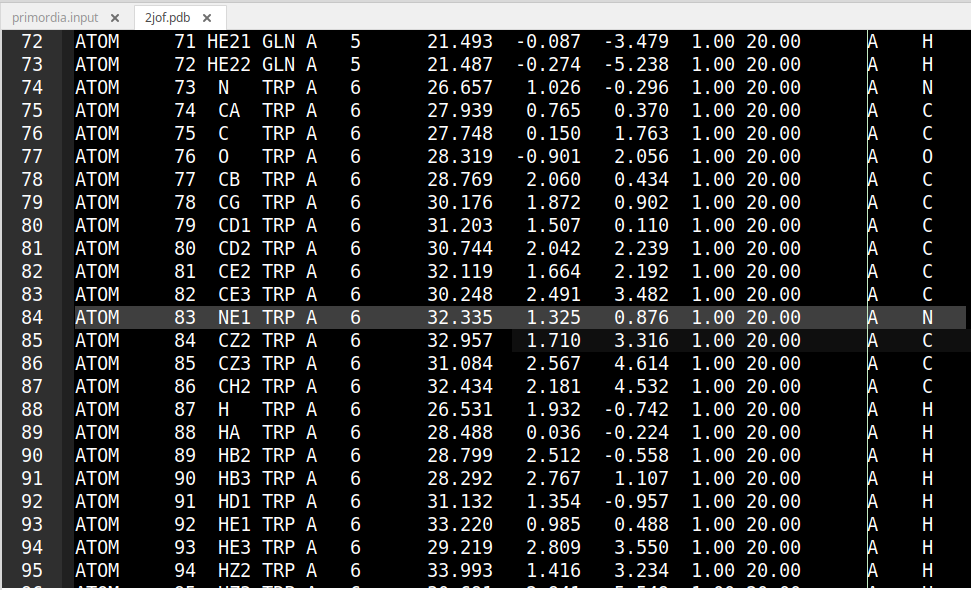
\includegraphics[width=4in]{images/tut3_img3}
\caption{Arquivo de PDB da TRP-cage aberta em editor de texto.}
\label{fig_tut3_2}
\end{center}
\end{figure}
\end{minipage}

Vamos modificar manualmente o input com esses dados de coordenada e tamanho de caixa 10 angstroms, com o input ficando assim como mostrado na caixa de texto \autoref{tut302}.

\hspace*{-1\leftmarginwidth}
\begin{minipage}{\fullwidth}
\begin{lstlisting}[caption={Input editado para execução do tutorial 3},label={tut302}]
#RT normal 
#PR eband 1 extrard pymols 
3 2jof_PM7.aux true 40 0 2jof_PM7.pdb mopac 32.335 1.325 0.876 10 EW 
3 2jof_PM7_lmo.aux true 40 10 2jof_PM7_lmo.pdb mopac 0 0 0 0 BD	
\end{lstlisting}
\end{minipage}

Finalmente, com esse input podemos colocar o programa para rodar com o seguinte cálculo

\hspace*{-\leftmarginwidth}
\begin{minipage}{\fullwidth}
	\begin{commandshell}path/to/PRIMoRDiA_1.25v_LINUX64 -f primordia.input\end{commandshell}
\end{minipage}

O programa deve finalizar a sua execução sem erros e produzir vários arquivos no diretório, com extensão ".cube', ".pym", ".lrd" e etc. Vamos explicar os arquivos com os resultados de descritores e como analisá-los na próxima seção desse tutorial.

\subsection{Análises dos Resultados}

Dos resultados produzidos temos os descritores globais, locais em representação condensada ( arquivos ".lrd" ), locais em representação volumétrica ( arquivos ".cube" ) e locais condensados escritos em PDB (nas pastas "RD\_PDB"). Para macromoléculas é interessante observar os descritores globais mais por uma questão de acompanhamento da normalidade do cálculo quântico executado, pois os processos nesses sistemas tendem a ser somente locais, tendo pouca relevância a propensão de uma proteína inteira de transferir ou receber elétrons. Por isso vamos passar a análise do arquivo "primordia.global".

Para esse lançamento estável do programa, PRIMoRDiA 1.25v, a principal modificação é a consolidação dos scripts de automatização de análise e produção de resultados com qualidade de publicação, usando o pacote gráfico Pymol e o pacote estatístico R. Por isso, nos próximos passos do tutorial, vamos focar na produção de imagens a partir desses scripts.

\subsubsection{Descritores Condensados} 

Descritores locais são funções matemáticas dependente de coordenadas espaciais, descrevendo as tendências de um certo ponto no espaço molecular. No caso dos descritores condensados, esses valores são particionados para cada centro atômico, simplificando a interpretação dos resultados, e para o caso de grandes sistemas, tornando a visualização mais clara, já que a representação volumétrica para sistemas de proteínas e afins pode ficar bem poluída.

No entanto, esse tipo de representação pode ser bem complicada de trabalhar, já que é uma lista de valores por átomos, ou seja, uma tabela que pode ser significativamente grande para macromoléculas. Pensando em facilitar a análise dessas resultados, o PRIMoRDiA escreve um arquivo de PDB para cada descritor calculado com os valores no campo do b-factor, e assim podemos usar o pacote gráfico Pymol para visualizar os descritores colorindo os átomos com uma paleta customizada. Para operar o Pymol mais automaticamente possível, o PRIMoRDiA escreve um arquivo de script com o sufixo "\_pymols\_pdb.pym", com um exemplo de sua estrutura mostrado na \autoref{fig_tut3_3}.


\hspace*{-\leftmarginwidth}
\begin{minipage}{\fullwidth}
	\begin{figure}[H]
		\begin{center}
			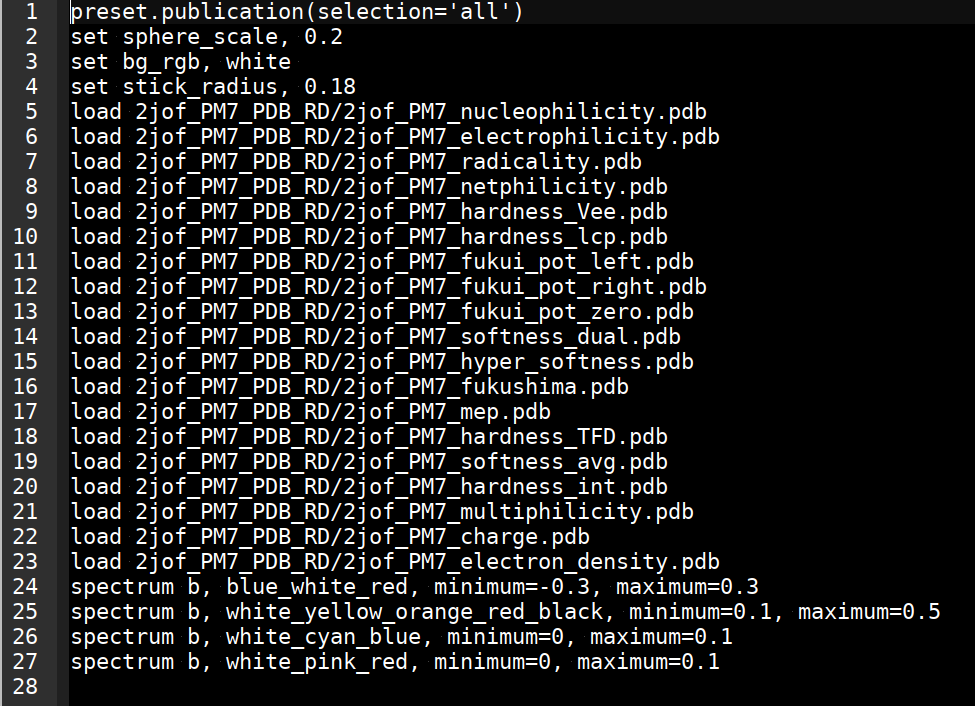
\includegraphics[width=4in]{images/tut3_img5}
			\caption{Script de automação da visualização dos descritores locais condensados no Pymol escrita no PRIMoRDiA e aberta em editor de texto.}
			\label{fig_tut3_3}
		\end{center}
	\end{figure}
\end{minipage}

Esse arquivo tem comandos para executar no Pymol modificando parâmetros de visualização e para carregar os PDBs com os descritores. Além disso ele já executa algumas paletas de cores, sendo que uma vai sobrepondo a outra, mas servem para o usuário pegar e escolher uma ou modificar seus parâmetros e cores. Abra o seu Pymol, execute o comando mostrado a baixo

\hspace*{-\leftmarginwidth}
\begin{minipage}{\fullwidth}
	\begin{pymol}@2jof_PM7_pymols_pdb.pym\end{pymol}
\end{minipage}

Depois da execução desse comando, a janela do pymol deve abrir e carregar todos os arquivos de PDB e executar todos os comandos que configuram a paleta de cores baseada nos valores dos descritores. O último comando de "spectrum b..." executada deve ser o que fica aparecendo, como na \autoref{fig_tut3_5}.

\hspace*{-\leftmarginwidth}
\begin{minipage}{\fullwidth}
\begin{figure}[H]
\begin{center}
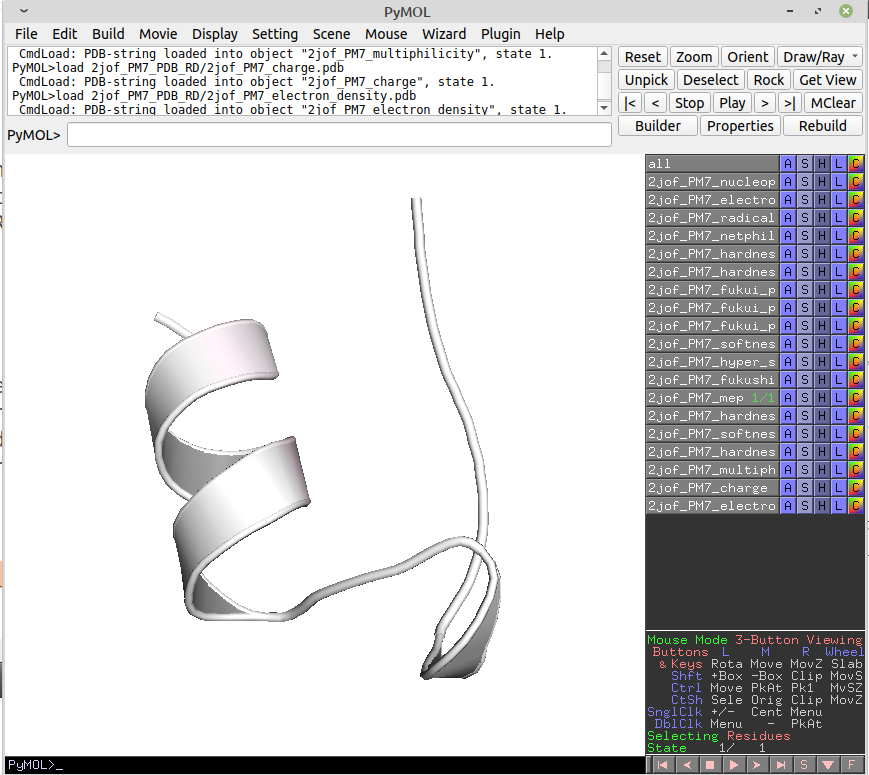
\includegraphics[width=3.3in]{images/tut3_img7}
\caption{Descritores locais condensados para a estrutura da TRP-cage carregados no Pymol.}
\label{fig_tut3_5}
\end{center}
\end{figure}
\end{minipage}

Na próxima imagem nós mostramos o Pymol com somente um dos objetos ativos, o 2jof\_PM7\_nucleophilicity, e mostrando o comando a ser executado no terminal, que foi selecionado/copiado a partir de um daqueles que foi executado quando o script foi chamado.


\hspace*{-\leftmarginwidth}
\begin{minipage}{\fullwidth}
	\begin{figure}[H]
		\begin{center}
			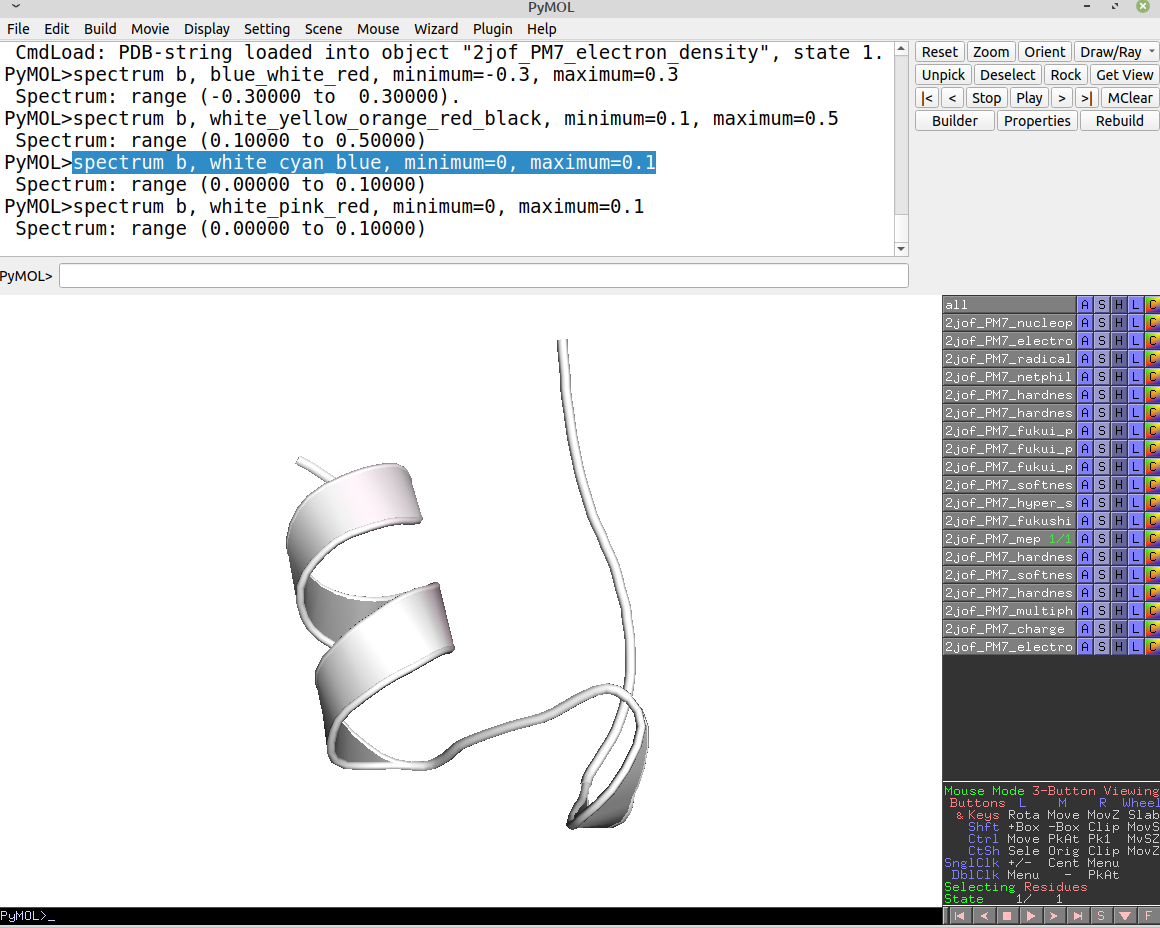
\includegraphics[width=3.5in]{images/tut3_img8}
			\caption{Janela do Pymol mostrando o comando que já tinha sido executado.}
			\label{fig_tut3_6}
		\end{center}
	\end{figure}
\end{minipage}

Depois de executar esse comando no Pymol o resultado é o mostrado \autoref{fig_tut3_7}, onde já é mostrado que os átomos de algumas cadeias laterais estão selecionados, já que somente a estrutura secundária está em evidência, com o próximo comando no Pymol os átomos selecionados aparecem em representação de bastões.

\hspace*{-\leftmarginwidth}
\begin{minipage}{\fullwidth}
	\begin{pymol}show sticks, sele\end{pymol}
\end{minipage}

\hspace*{-\leftmarginwidth}
\begin{minipage}{\fullwidth}
	\begin{figure}[H]
		\begin{center}
			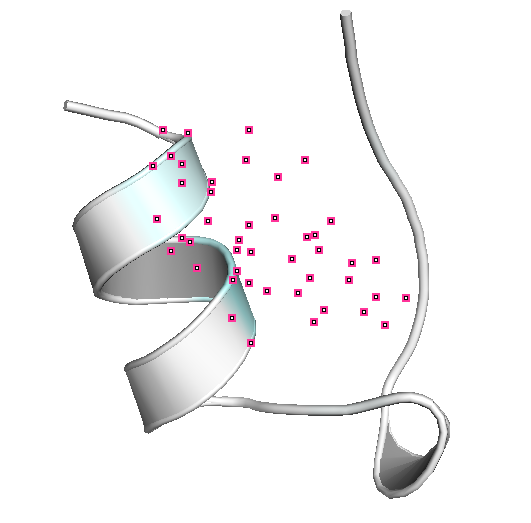
\includegraphics[width=3.5in]{images/tut3_img9}
			\caption{Estrutura no Pymol com duas cadeias laterais selecionadas.}
			\label{fig_tut3_7}
		\end{center}
	\end{figure}
\end{minipage}

Os átomos e ligações entre os mesmos serão mostrados na representação de sticks (bastões), resultando na figura \autoref{fig_tut3_9}, mostrando a estrutura pintada baseada nos valores de suscetibilidade a um ataque electrofílico, ou o mesmo que nucleofilicidade. Onde a cor azul está mais escuro é onde os valores são maiores, é possível alterar esses valores de máximo e mínimo bem como as cores também. Na figura abaixo é possível observar que o comando "ray" foi executado no Pymol. Escreva o mesmo e execute, depois de alguns segundos aparece um fundo de  transparência, significando que a imagem já foi renderizada e pode ser salva com o comando "png" como já usado para os descritores volumétricos nos tutoriais anteriores. 


\hspace*{-\leftmarginwidth}
\begin{minipage}{\fullwidth}
	\begin{figure}[H]
		\begin{center}
			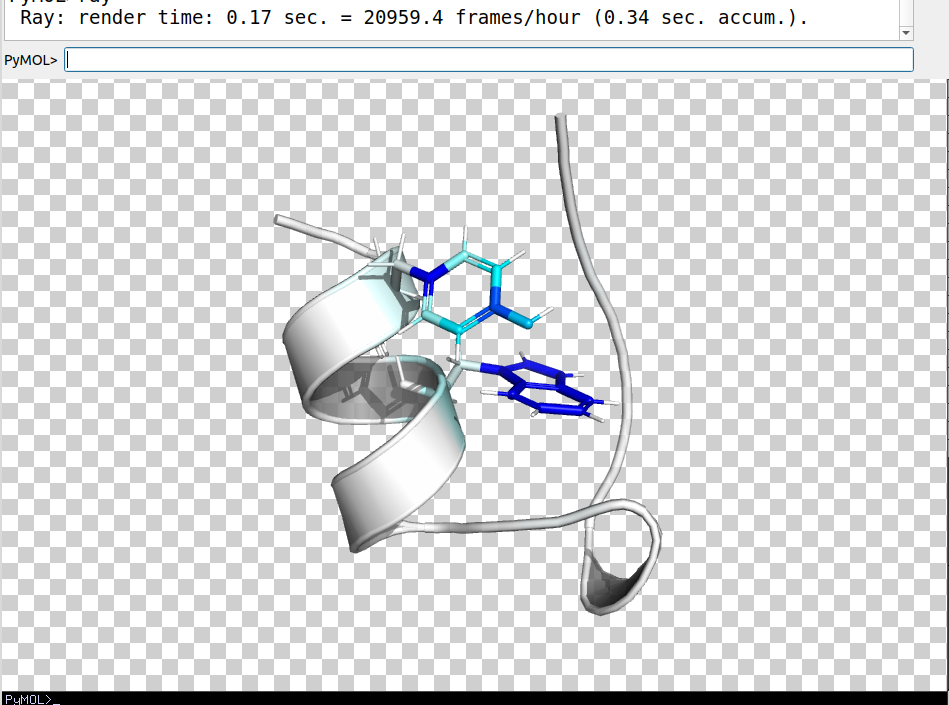
\includegraphics[width=3.5in]{images/tut3_img11}
			\caption{Representação do descritor local condensada nucleofilicidade para a estrutura da TRP-cage, com fundo de transparência, renderizada e pronta para ser salva em arquivo.}
			\label{fig_tut3_9}
		\end{center}
	\end{figure}
\end{minipage}

Esse processo de colorir os átomos, renderizar e salvar essas imagens pode ser repetido para todos os outros descritores. Para os descritores de dureza local é interessante utilizar outros modos de \emph{ray tracing}. Para próxima imagem mostrada, foi ativado no pymol o objeto 2jof\_PM7\_hardness\_B, e executado os seguintes comandos no Pymol

\hspace*{-\leftmarginwidth}
\begin{minipage}{\fullwidth}
	\begin{pymol}set ray_trace_mode=1\end{pymol}
\end{minipage}

\hspace*{-\leftmarginwidth}
\begin{minipage}{\fullwidth}
	\begin{pymol}show sticks\end{pymol}
\end{minipage}

\hspace*{-\leftmarginwidth}
\begin{minipage}{\fullwidth}
	\begin{pymol}set spectrum b,white_yellow_orange_red_black,minimum=0.1,maximum=0.2\end{pymol}
\end{minipage}

\hspace*{-\leftmarginwidth}
\begin{minipage}{\fullwidth}
	\begin{pymol}ray\end{pymol}
\end{minipage}

\hspace*{-\leftmarginwidth}
\begin{minipage}{\fullwidth}
	\begin{pymol}png 2jof_hardneess.png\end{pymol}
\end{minipage}

A imagem salva em disco deve ser similar a mostrada na \autoref{fig_tut3_11}, mostrando a dureza local para a estrutura da TRP-cage.  

\hspace*{-\leftmarginwidth}
\begin{minipage}{\fullwidth}
	\begin{figure}[H]
		\begin{center}
			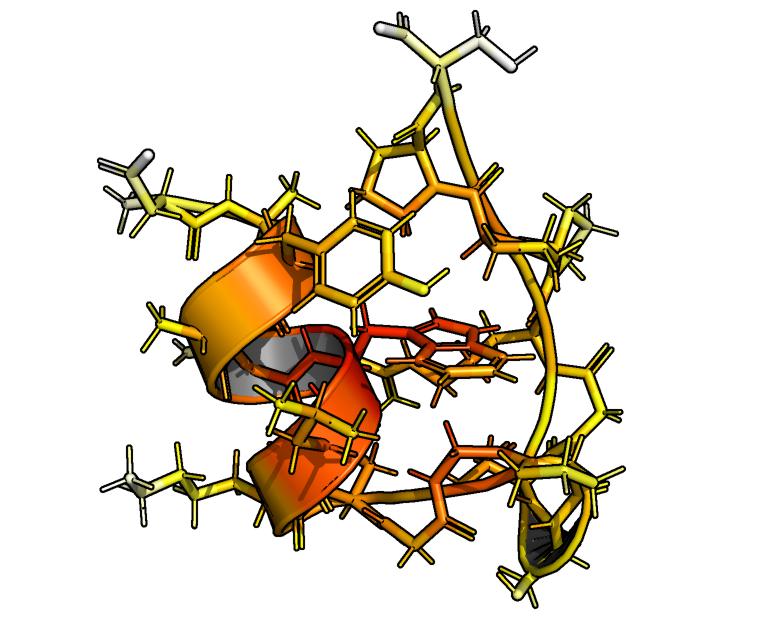
\includegraphics[width=3.5in]{images/tut3_img13}
			\caption{Imagem salva para a dureza local em representação condensada gerada no Pymol.}
			\label{fig_tut3_11}
		\end{center}
	\end{figure}
\end{minipage}


\subsubsection{Representação Volumétrica}


Os descritores com representação volumétrica seguem a mesma lógica de visualização que os outros dois últimos tutoriais. A diferença, no caso dos cálculos específicos para macromoléculas, através dos métodos BD e EW, é na seleção e combinação dos orbitais moleculares. Para automatizar a visualização dos descritores básicos em representação volumétrica, o PRIMoRDiA escreve um script semelhante ao mostrado na \autoref{fig_tut3_13}, que é para a entrada 2jof\_PM7\_lmo.aux. Para a outra entrada, 2jof\_PM7.aux, também foi escrito um script desses, que depois de ser executado abre as estruturas e renderiza os cubes no Pymol como na \autoref{fig_tut3_15}.


\hspace*{-\leftmarginwidth}
\begin{minipage}{\fullwidth}
	\begin{figure}[H]
		\begin{center}
			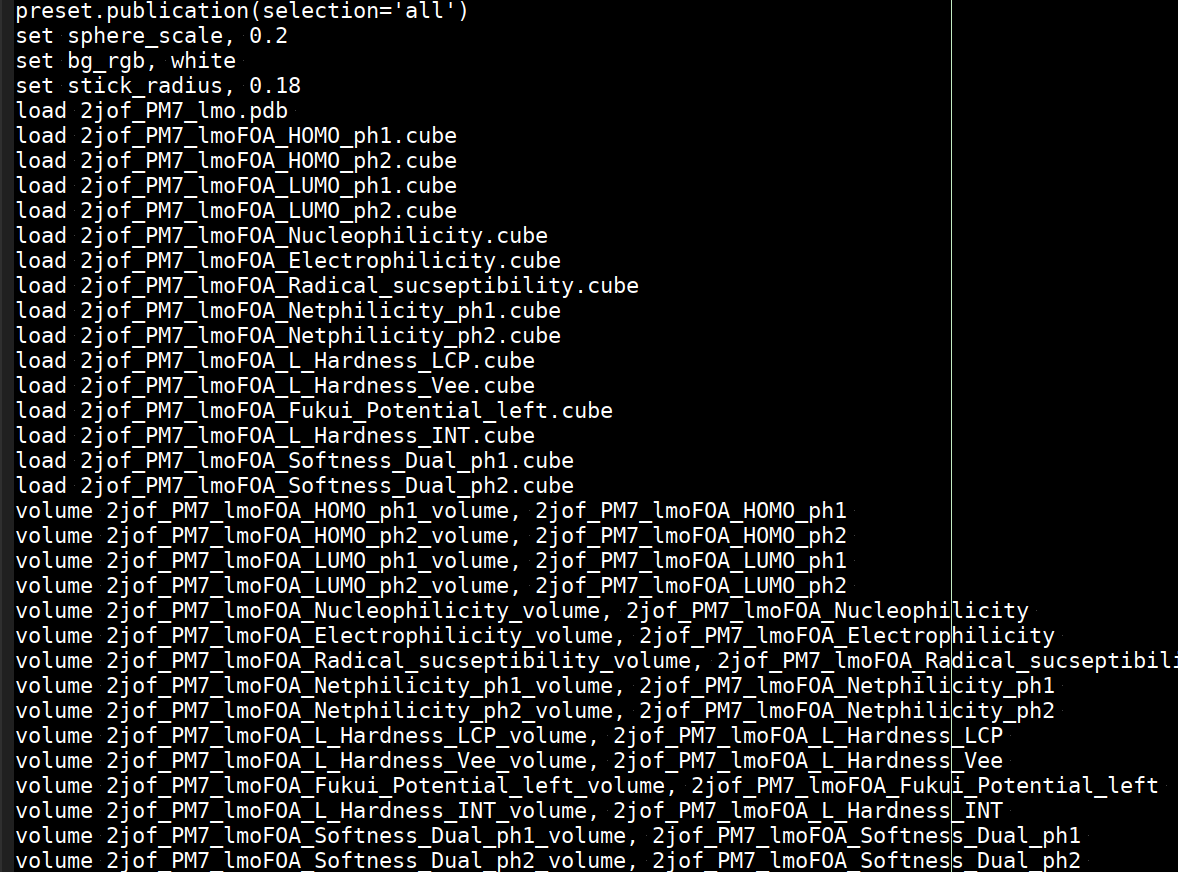
\includegraphics[width=4in]{images/tut3_img15}
			\caption{Parte do script de automação da visualização dos descritores locais volumétricos no Pymol escrita no PRIMoRDiA e aberta em editor de texto.}
			\label{fig_tut3_13}
		\end{center}
	\end{figure}
\end{minipage}


Na \autoref{fig_tut3_15} já nos adiantamos e selecionamos só as fases do descrito de netfilicidade, lembrando que todos os descritores que possuem valores negativos e positivos são escritos em dois arquivos idênticos, mas com nomes diferentes, para que o Pymol renderize separadamente. Também, na mesma imagem é possível ver que já tem algumas cadeias laterais já selecionada, que são aqueles que é possível perceber que os volumes estão renderizados sobre seus átomos. 

\hspace*{-\leftmarginwidth}
\begin{minipage}{\fullwidth}
	\begin{figure}[H]
		\begin{center}
			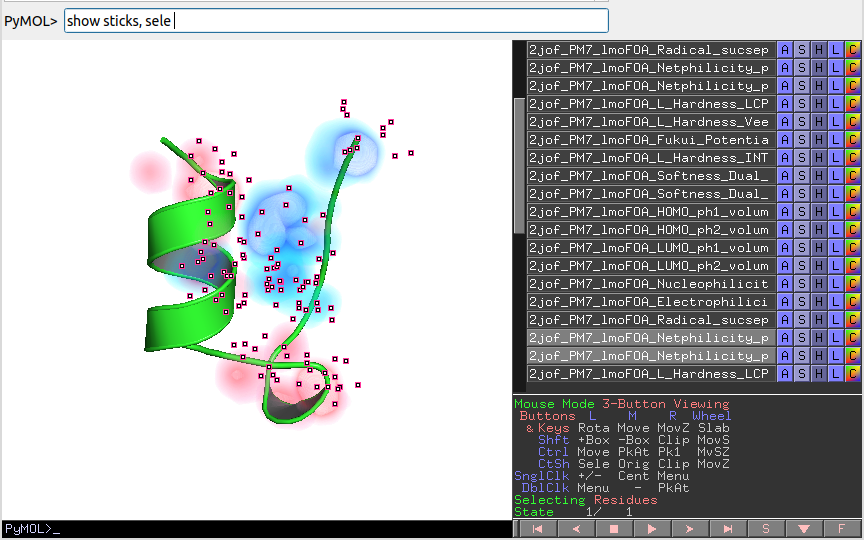
\includegraphics[width=4in]{images/tut3_img17}
			\caption{Janela do Pymol mostrando os descritores locais volumétricos carregadas pelo script gerado no PRIMoRDiA para a estrutura da TRP-cage com alguns resíduos selecionados.}
			\label{fig_tut3_15}
		\end{center}
	\end{figure}
\end{minipage}

Na área de comando do Pymol mostrado na \autoref{fig_tut3_15} aparece o comando para que a representação de bastões seja ativada para essas cadeias selecionadas. Depois desse comando ser executados os bastões aparecem como mostrado na \autoref{fig_tut3_17}. O comando de \emph{draw} pode ser utilizado para renderizar e de depois salvar a imagem em disco com o comando \emph{png}, como já exemplificado nos tutoriais 1 e 2. 


\hspace*{-\leftmarginwidth}
\begin{minipage}{\fullwidth}
	\begin{figure}[H]
		\begin{center}
			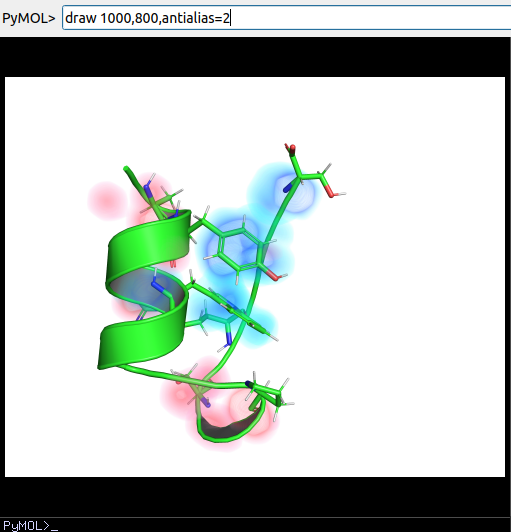
\includegraphics[width=4in]{images/tut3_img19}
			\caption{Janela do Pymol mostrando os descritores locais volumétricos carregadas pelo script gerado no PRIMoRDiA para a estrutura da TRP-cage com alguns resíduos mostrados em representação de bastões.}
			\label{fig_tut3_17}
		\end{center}
	\end{figure}
\end{minipage}

Agora vamos visualizar os resultados dos descritores calculados para a caixa definida no arquivo de input, executando o script do Pymol corresponde para essa entrada. O resultado deve ser como o apresentado na \autoref{fig_tut3_23}, carregando e renderizando vários descritores para a região limitada. 

\hspace*{-\leftmarginwidth}
\begin{minipage}{\fullwidth}
	\begin{figure}[H]
		\begin{center}
			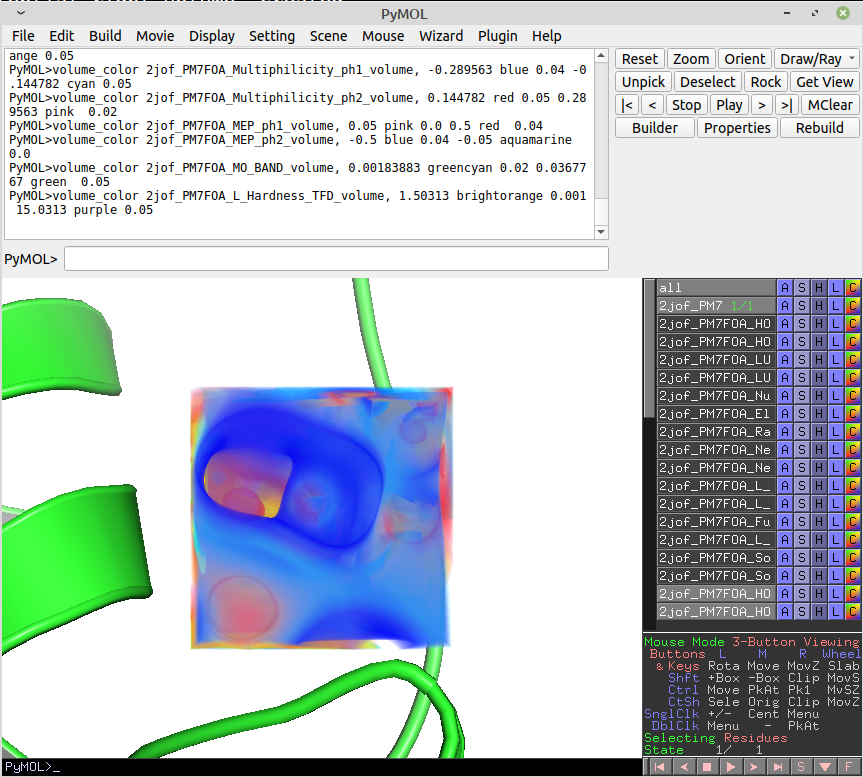
\includegraphics[width=4in]{images/tut3_img24}
			\caption{Janela do Pymol mostrando os descritores locais volumétricos carregadas pelo script gerado no PRIMoRDiA para um região cúbica específica da TRP-cage.}
			\label{fig_tut3_23}
		\end{center}
	\end{figure}
\end{minipage}

Se desativarmos todos os objetos de volume, ficamos só com os objetos de cube carregados, que no visualizador apareceram marcando as arestas dos limites do cube. Na \autoref{fig_tut3_24}, mostramos esse limite em vermelho, com uma cor diferente para chamar atenção. 

\hspace*{-\leftmarginwidth}
\begin{minipage}{\fullwidth}
	\begin{figure}[H]
		\begin{center}
			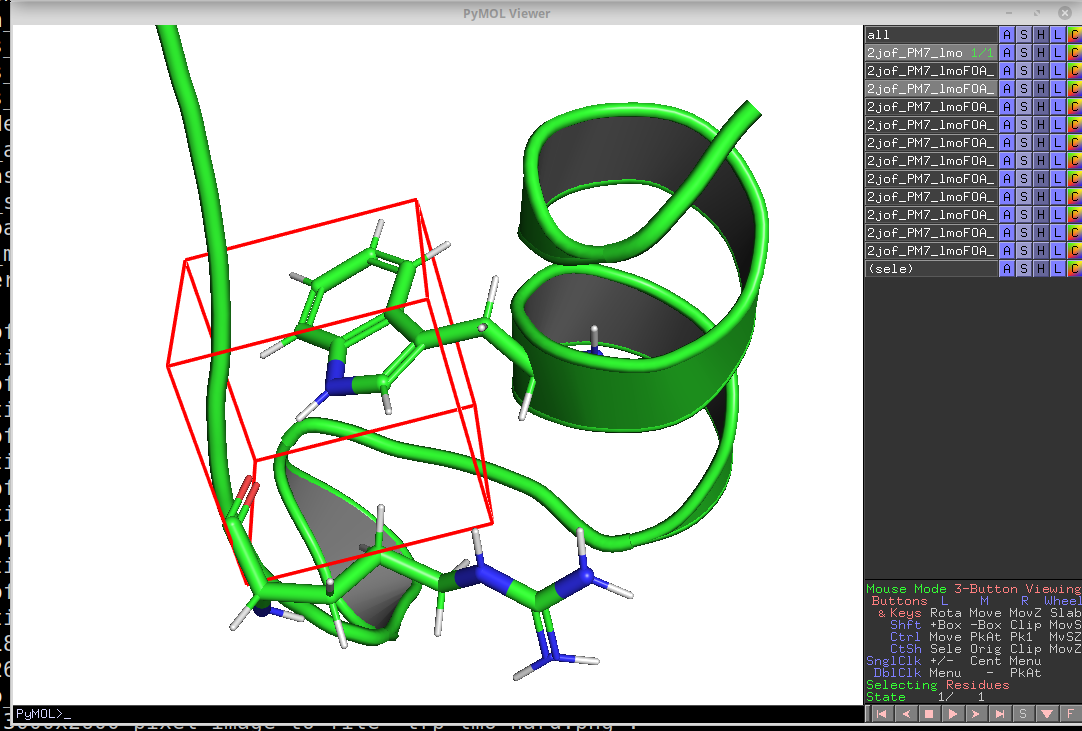
\includegraphics[width=4in]{images/tut3_img25}
			\caption{.}
			\label{fig_tut3_24}
		\end{center}
	\end{figure}
\end{minipage}

Em relação ao outros descritores volumétricos, os definidos dentro desses espaços limitados pelo usuário, não apresentam nenhuma diferença prática. A questão aqui é que com sistemas com um grande número de átomos é possível visualizar os descritores para regiões específicas sem perder resolução e que possam ser calculados em um tempo praticável. Nas próximas figuras estão apresentados alguns descritores renderizados para esse região delimitada e já salvas em qualidade de publicação dentro do pymol. Na \autoref{fig_tut3_25}, o descritor de dureza local utilizando a aproximação baseada no potencial químico local. Na \autoref{fig_tut3_25}, mostramos esse volume renderizad com uma paleta diferente, realçando melhor as regiões que apresentam valores maiores que outros. 

\hspace*{-\leftmarginwidth}
\begin{minipage}{\fullwidth}
	\begin{figure}[H]
		\begin{center}
			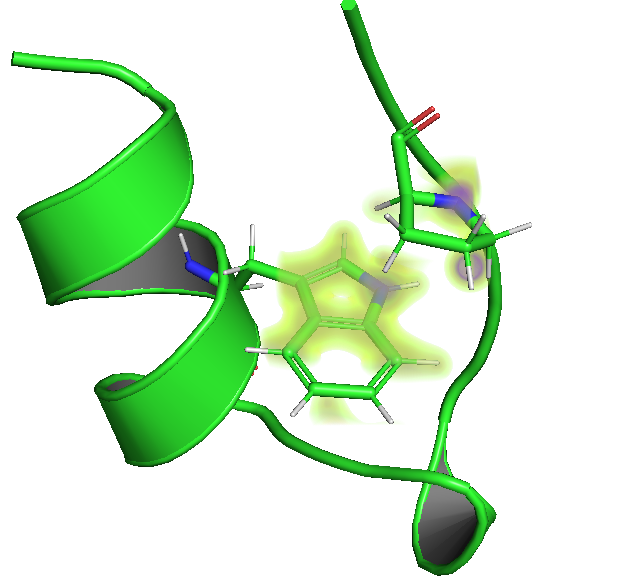
\includegraphics[width=4in]{images/tut3_img26}
			\caption{Exemplo de imagem do descritor renderizada para a região delimitada pelo usuário. Dureza local baseada na aproximação do potencial químico local.}
			\label{fig_tut3_25}
		\end{center}
	\end{figure}
\end{minipage}

\hspace*{-\leftmarginwidth}
\begin{minipage}{\fullwidth}
	\begin{figure}[H]
		\begin{center}
			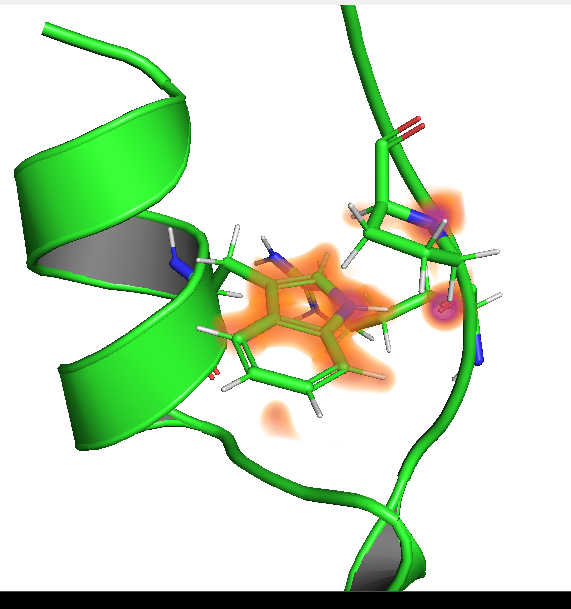
\includegraphics[width=3.5in]{images/tut3_img27}
			\caption{Exemplo de imagem do descritor renderizada para a região delimitada pelo usuário. Dureza local baseada na aproximação do potencial químico local.}
			\label{fig_tut3_26}
		\end{center}
	\end{figure}
\end{minipage}

Na \autoref{fig_tut3_27}, a última imagem é ampliada e a distância entre o hidrogênio da cadeia lateral e oxigênio do resíduo da cadeia principal é evidenciada, mostrando que nessa região onde claramente há uma ligação de hidrogênio também apresenta os maiores valores do descritor de dureza local em questão.  

\hspace*{-\leftmarginwidth}
\begin{minipage}{\fullwidth}
	\begin{figure}[H]
		\begin{center}
			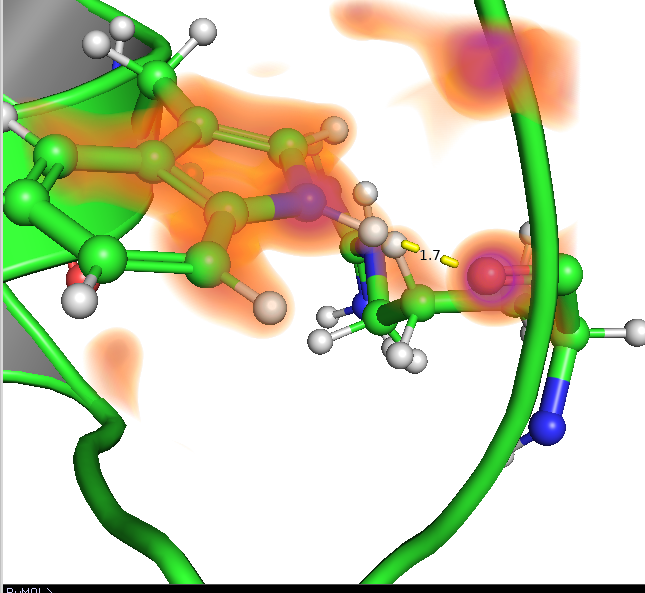
\includegraphics[width=3.5in]{images/tut3_img28}
			\caption{Exemplo de imagem do descritor renderizada para a região delimitada pelo usuário. Imagem ampliada para a região de interação de por ligação de hidrogênio, evidenciando a distância entre os átomos. Dureza local baseada na aproximação do potencial químico local.}
			\label{fig_tut3_27}
		\end{center}
	\end{figure}
\end{minipage}

\subsection{Representação Especial Para Resíduos e Densidade de Estados}

Para macromoléculas biológicas há diversas análises focadas em propriedades e estatísticas em função dos monômeros que os compõem. Na grande maioria, esses sistemas são proteínas que são compostas de fragmentos de amino-ácidos, chamados de resíduos de amino-ácidos. Da mesma forma que já apresentamos os descritores condensados para os átomos, é interessante analisar esses valores para cada um desses fragmentos do sistema. PRIMoRDiA utiliza as informações do PDB para somar os descritores dos átomos por resíduo e escrever em um arquivo formatado, como na \autoref{fig_tut3_28}. 

\hspace*{-\leftmarginwidth}
\begin{minipage}{\fullwidth}
	\begin{figure}[H]
		\begin{center}
			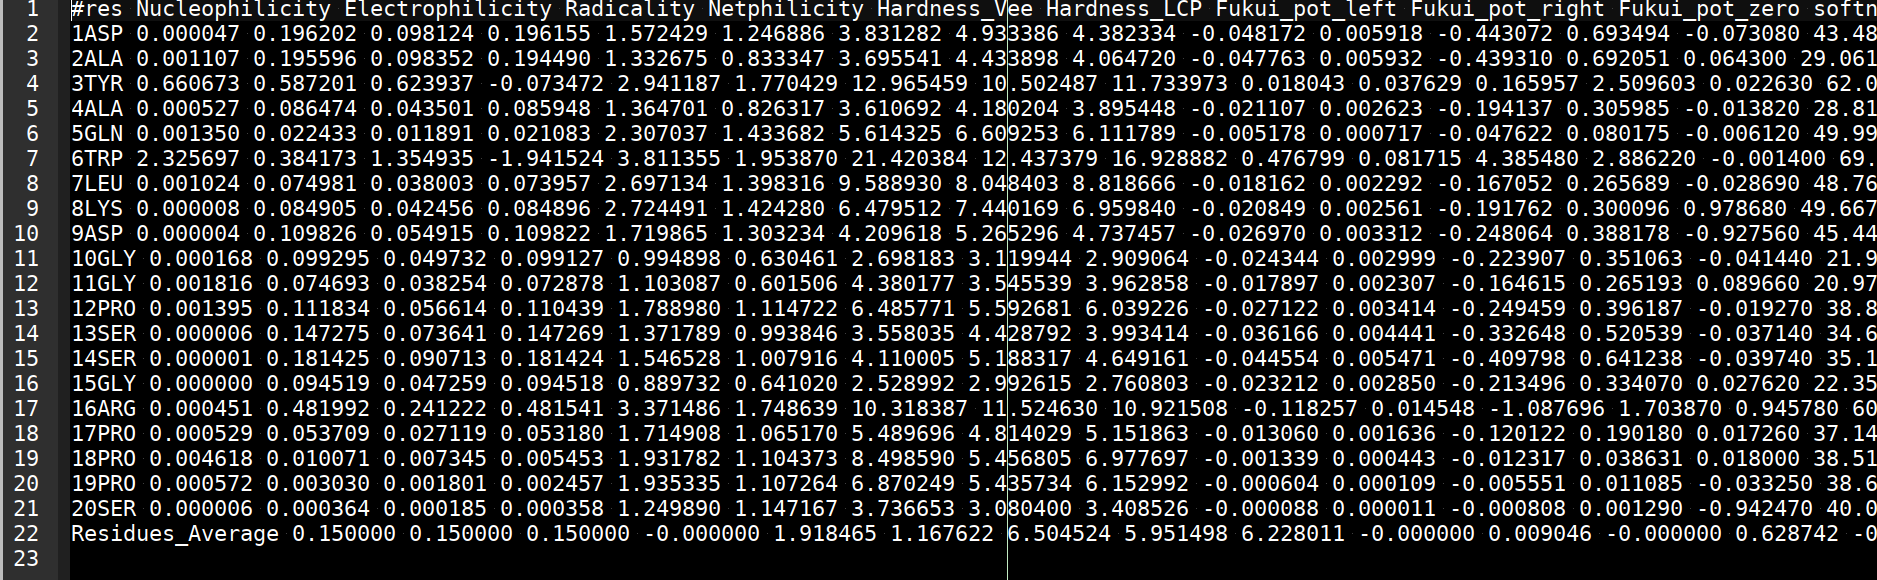
\includegraphics[width=6in]{images/tut3_img29}
			\caption{Arquivo com os descritores locais condensados por resíduo ( fragmento de amino-ácido ) para a estrutura da TRP-cage aberto em editor de texto.}
			\label{fig_tut3_28}
		\end{center}
	\end{figure}
\end{minipage}

Esses dados podem ser facilmente selecionados/copiados e transferidos para uma tabela de excel/libreoffice, como é exemplificado na \autoref{fig_tut3_29}. Para uma dada trajetória, de dinâmica molecular ou coordenada de reação, valores para resíduos específicos podem ser reunidos e analisados durante esses processos. Mais sobre isso é exemplificado no tutorial 5.

\hspace*{-\leftmarginwidth}
\begin{minipage}{\fullwidth}
	\begin{figure}[H]
		\begin{center}
			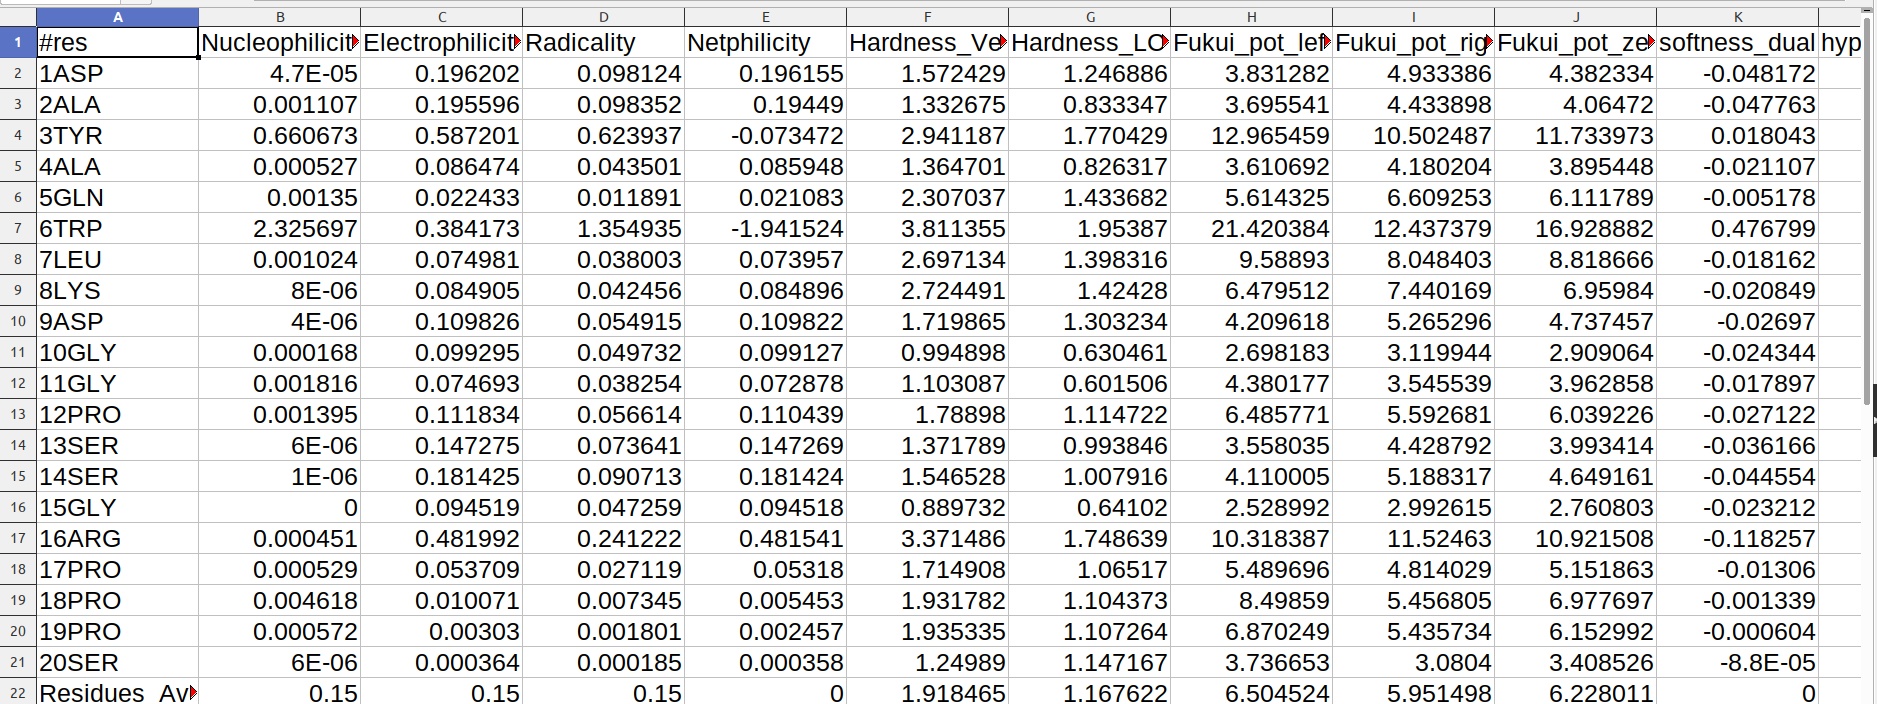
\includegraphics[width=5in]{images/tut3_img30}
			\caption{Planilha eletrônica com os descritores locais condensados por resíduo ( fragmento de amino-ácido ) para a estrutura da TRP-cage.}
			\label{fig_tut3_29}
		\end{center}
	\end{figure}
\end{minipage}

Através da análise desses dados numéricos, é possível indicar a reatividade de sistemas biológicos pelo seus resíduos, o que é muito útil na hora de definir domínios importantes para enzimas, como sitio ativo, sitio de ligação, sitio alostérico e etc. Além disso, essas tabelas de dados são ricas em informações para algorítimos de aprendizagem de máquina, com propriedades eletrônicas calculadas por métodos quânticos para monômeros dos sistemas. 

Uma das funcionalidades do PRIMoRDiA é escrever uma tabela de energia e um script para ser executado em R para a produção de um gráfico de densidade de estados de energia. A análise desses dados é interessante para biopolímeros, devido a alta concentração de níveis de energia com a energia similar ao do HOMO e LUMO. Esse script é produzido quando a keyword "dos" é utilizada no campo de parâmetros do input e pode ser útil para avaliar o número de orbitais máximos utilizados ou a valor de corte de energia para contabilização dos orbitais moleculares.

Na pasta desse tutorial, depois que o input foi executado, deve ter arquivos com final "DOS.R" e "DOS". Para gerar uma imagem automaticamente com o script é só executar o comando

\hspace*{-\leftmarginwidth}
\begin{minipage}{\fullwidth}
	\begin{commandshell}Rscript 2jof_PM7_lmo_DOS.R\end{commandshell}
\end{minipage}

E na pasta deve aparecer uma imagem como a figura abaixo

\hspace*{-\leftmarginwidth}
\begin{minipage}{\fullwidth}
	\begin{figure}[H]
		\begin{center}
			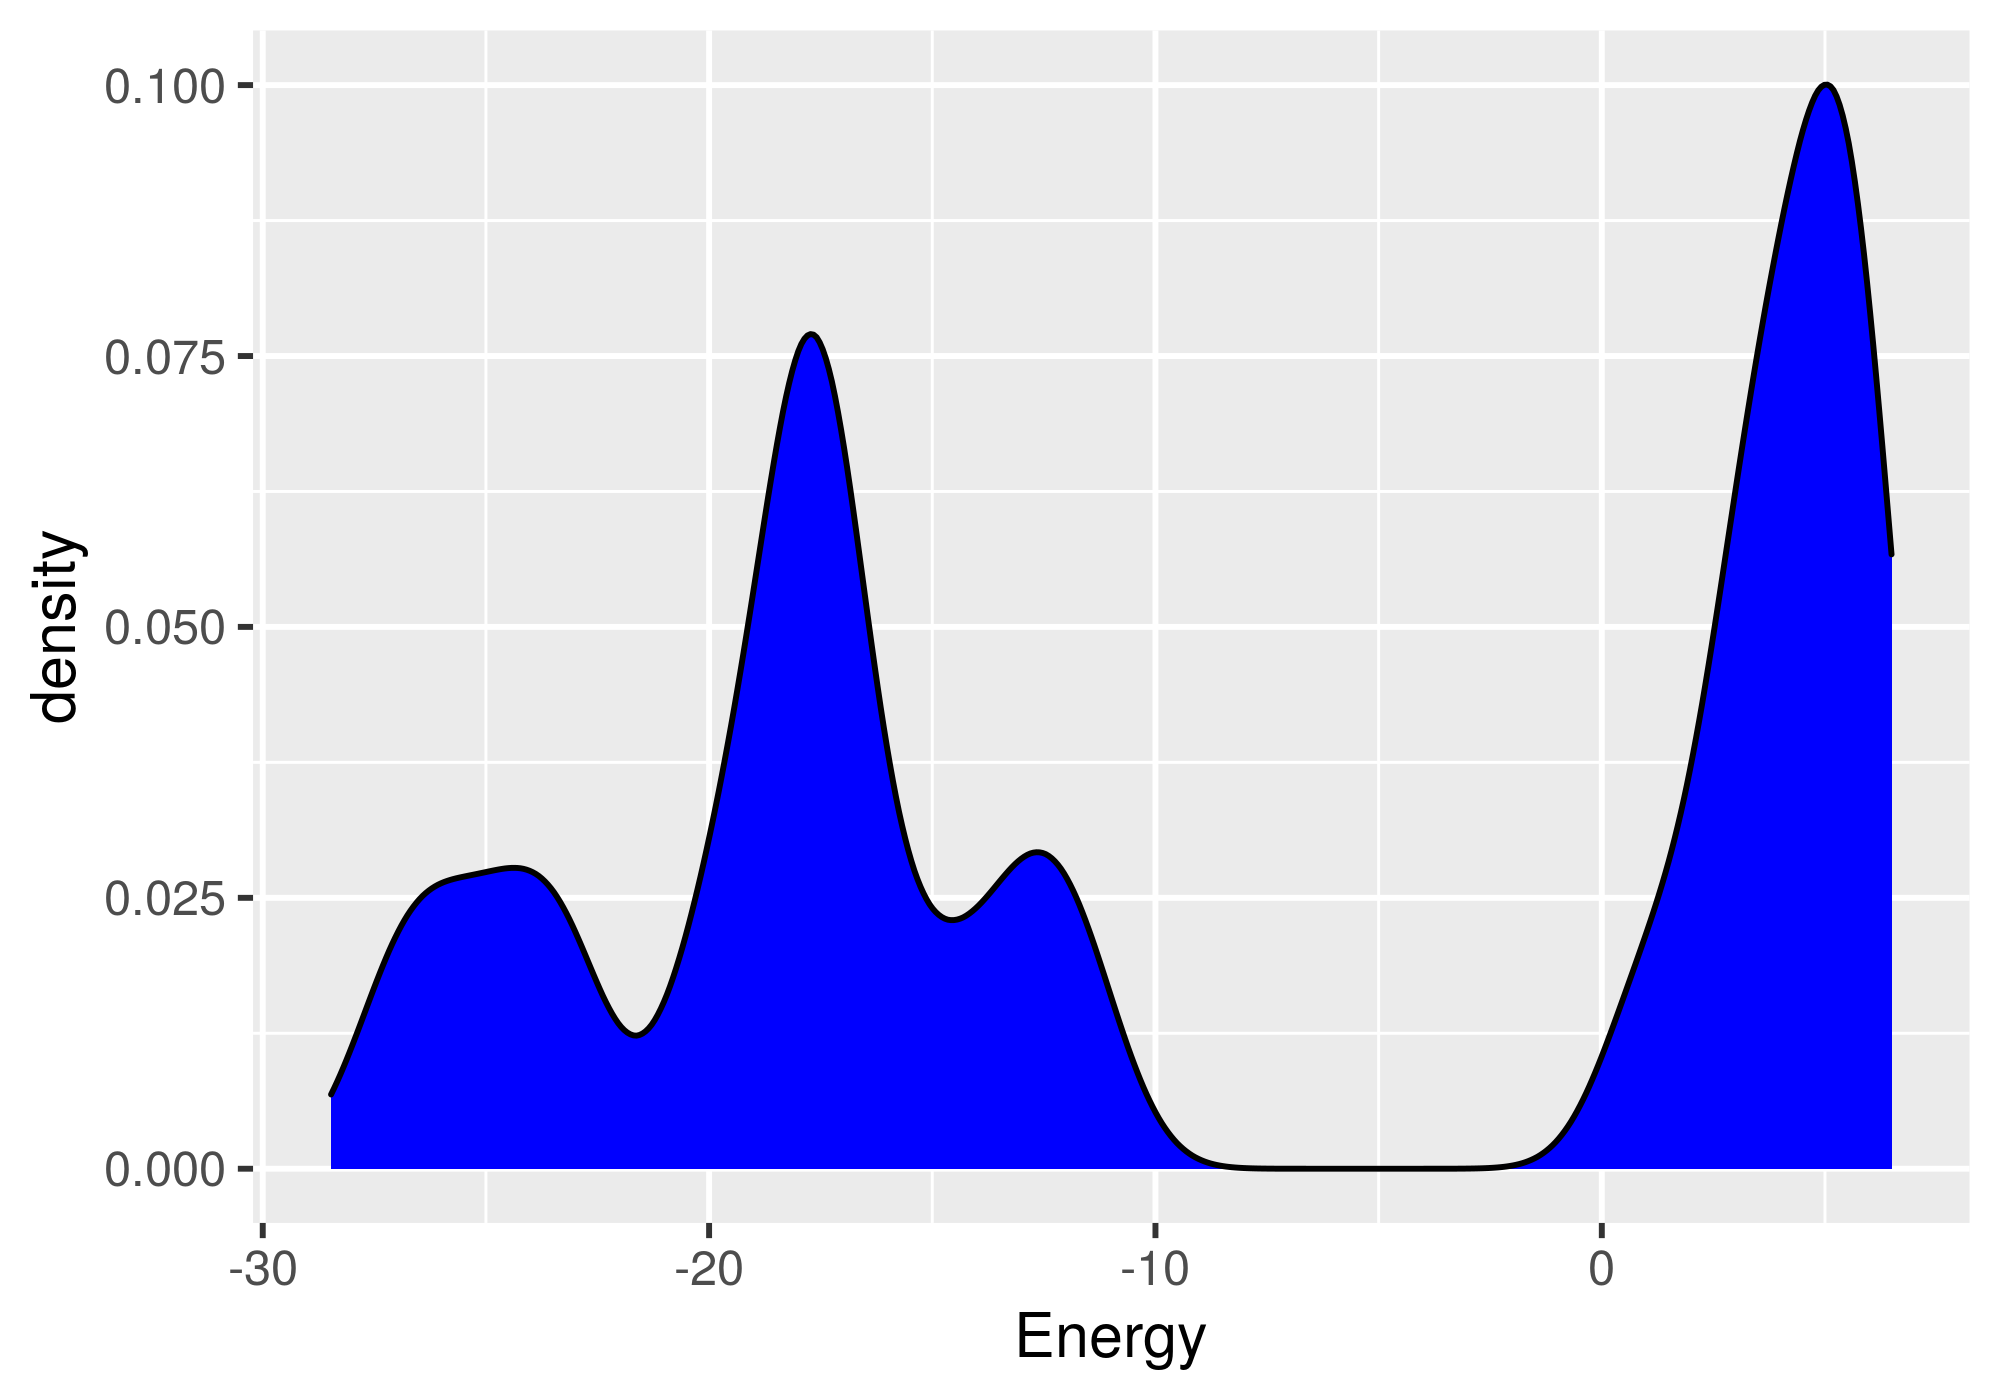
\includegraphics[width=3.4in]{images/tut3_img31}
			\caption{Gráfico de densidade de estados de energia para os orbitais moleculares da TRP-Cage calculados com PM7 junto com algorítimo MOZYME.}
			\label{fig_tut3_30}
		\end{center}
	\end{figure}
\end{minipage}

E o comando abaixo cria a figura da densidade de estados para a TRP calculada normalmente com o PM7

\hspace*{-\leftmarginwidth}
\begin{minipage}{\fullwidth}
	\begin{commandshell}Rscript 2jof_PM7_DOS.R\end{commandshell}
\end{minipage}


\hspace*{-\leftmarginwidth}
\begin{minipage}{\fullwidth}
	\begin{figure}[H]
		\begin{center}
			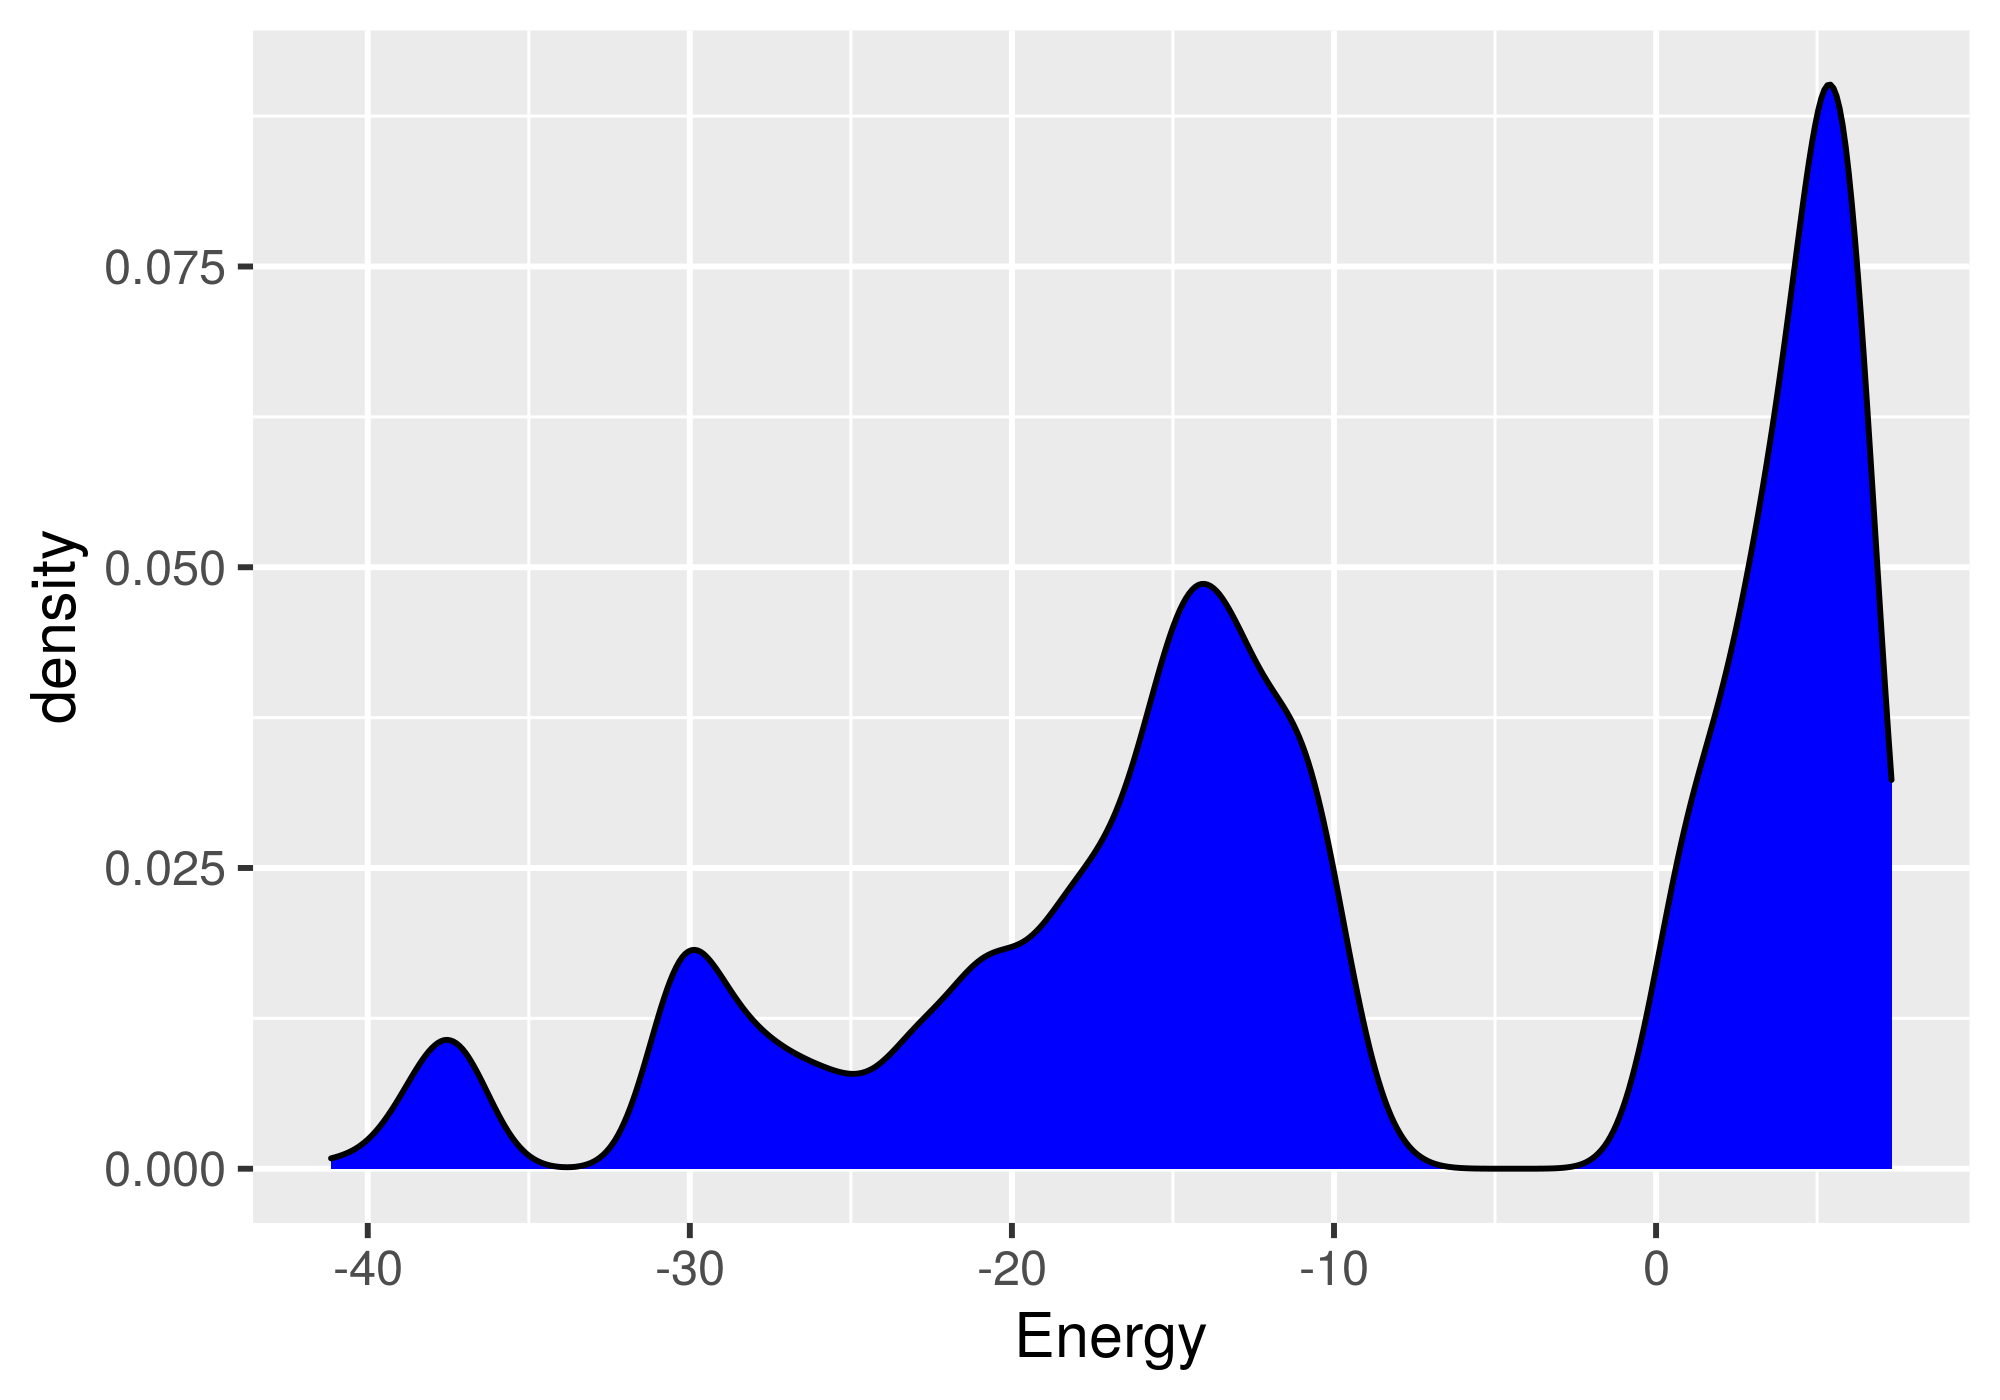
\includegraphics[width=3.4in]{images/tut3_img32}
			\caption{Gráfico de densidade de estados de energia para os orbitais moleculares da TRP-Cage calculados com PM7.}
			\label{fig_tut3_31}
		\end{center}
	\end{figure}
\end{minipage}

Nós podemos observar que os valores de energia dos orbitais cálculados com o algoritmo MOZYME, são mais concentrados que os que não utilizaram essa estratégia de aceleração dos cálculos. Isso faz com que o gap HOMO-LUMO fique maior nesse primeiro caso, o que acaba alterando bastante na hora de escolher os orbitais moleculares para combinar na hora de calcular os descritores. Portanto, o ideal para sistemas novos é sempre que possível fazer a análise desse gráfico que facilmente pode ser produzido com a ajuda do PRIMoRDiA.   

\newpage
\section{Tutorial 4: Análise de Força Ácida}

Esse tutorial segue a mesma lógica do Tutorial 1, mas focado na interpretação dos resultados. Como nesse primeiro. Vamos demonstrar como utilizar o programa para obter os descritores de reatividade usando as informações dos orbitais moleculares de fronteira, opção 1 de cálculo do PRIMoRDiA, partindo de cálculos semiempiricos no MOPAC, para quatro aminoácidos,  gerando descritores de reatividade que podem ser utilizados para explicar os locais preferenciais de protonação.

\subsection{Contextualização}

Aminoácidos são moléculas orgânicas anfóteras, isto é, podem agir como ácidos e bases, devido aos grupos amina e ácido carboxílico. Além disso, alguns tem cadeias laterais que são considerados como ácidos ou bases, e quando estão na composição de uma proteína essa acidez/basicidade vai ser relevante para diversos processos e propriedades.

A força ácida é medida pelo pKa, que é o negativo do log da constante de força ácida. De forma resumida, quando o pH está menor que o pKa de um grupo da molécula esse grupo tende a ficar protonado, em caso contrário sem esse próton. Ou seja, quanto menor o pKa mais ácido e quanto maior mais básico. No entanto, as medidas de pKa mudam com o ambiente químico e a sua obtenção de forma teórica apresenta diversos desafios quando os sistemas envolvidos são proteínas.

Os descritores podem ser úteis para identificar locais nas moléculas para sítios preferências para transferência de elétrons. Mais especificativamente, a dureza local é o descritor ideal para transferência de prótons, que é um partícula pequena carregada e portanto dominado por interações de natureza eletrostática. Nesse tutorial, vamos calcular os descritores para uma cisteína, ácido aspártico, ácido glutâmico e uma lisina, e cruzar com dados de pKa e potencial de ionização.


\subsection{Arquivos Necessários e Execução}

Todos os arquivos necessários para a execução se encontram na pasta comprimida fornecida junto ao programa, sendo eles os aquivos que contém as informações de saída do programa MOPAC para os quatro amino-ácidos estudados. Assim também como um arquivo de input com as mesmas linhas de texto que mostradas abaixo. 

\hspace*{-\leftmarginwidth}
\begin{minipage}{\fullwidth}
\begin{lstlisting}[caption={Input editado para execução do tutorial 3},label={tut402}]
#RT normal 
#PR pymols
1 asp.aux true 40 mopac
1 cys.aux true 40 mopac
1 glu.aux true 40 mopac
1 lys.aux true 40 mopac
\end{lstlisting}
\end{minipage}

Como já mostrado nos tutoriais anteriores, depois de ter o input na pasta onde estão os arquivos é só rodar o programa com a flag "-f". Depois disso os arquivos com os resultados devem criados na pasta. 

\subsection{Análise dos Resultados}

Os resultados para esse tutorial são bem parecidos com os obtidos no tutorial 1, sendo que utilizamos a mesma opção de cálculo para geração dos descritores com aproximação de orbitais congelados. Na \autoref{fig_tut1_4} é mostrada o arquivo de texto com os resultados dos descritores globais, na \autoref{fig_tut1_5} os mesmos dados transpostos para um planilha do Libre Office.  

\hspace*{-\leftmarginwidth}
\begin{minipage}{\fullwidth}
	\begin{figure}[H]
		\begin{center}
			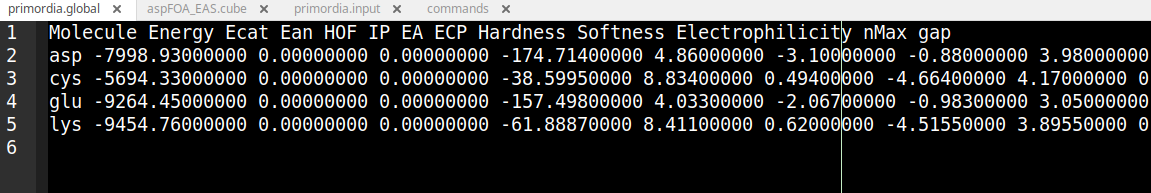
\includegraphics[width=6in]{images/tut4_img3}
			\caption{Arquivo de texto com os resultados dos  descritores globais para os amino-ácidos calculados.}
			\label{fig_tut4_1}
		\end{center}
	\end{figure}
\end{minipage}

\hspace*{-\leftmarginwidth}
\begin{minipage}{\fullwidth}
	\begin{figure}[H]
		\begin{center}
			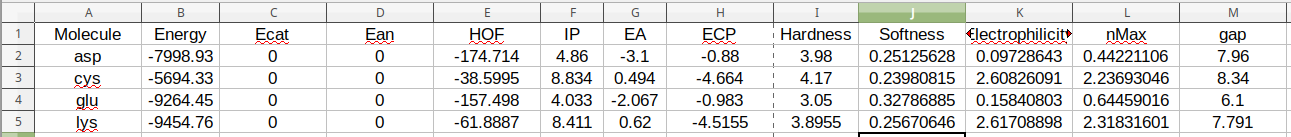
\includegraphics[width=6in]{images/tut4_img4}
			\caption{Planilha com os resultados dos descritores globais para os amino-ácidos calculados.}
			\label{fig_tut4_2}
		\end{center}
	\end{figure}
\end{minipage}

O que pode ser extraído desses resultados é que para o mesmo método de estrutura eletrônica as moléculas de lisina e ácido aspártico tem dureza química bem próximas, a cisteína com uma dureza bem maior que todos e o ácido glutâmico com a menor. De fato, o ácido glutâmico tem dois oxigênios que geralmente em ambientes enzimáticos agem como aceptores de prótons e/ou participando em ataques nucleofílicos. Entretanto, por mais que a cisteína se apresente como mais dura nesses resultados, é o amino-ácido com a maior capacidade de receber elétrons junto com a lisina. 

Já para os descritores locais, para cada molécula calculada foi gerado um arquivo ".lrd", como já explicado em tutoriais anteriores como explora-los e analisa-los em planilhas. Os dados dos descritores locais mais apropriados para avaliar a força ácida vão ser reunidas posteriormente para os átomos aceptores/receptores de prótons. 

Para ajudar de forma qualitativa na análise, podemos gerar os descritores volumétricos no pacote gráfico Pymol. Isso pode ser facilmente realizado usando os scripts gerados pelo PRIMoRDiA, como já vimos em outros tutoriais. Abra o Pymol e execute the ".pymols" script no terminal do programa. O resultado deve ser o parecido com o mostrado na \autoref{fig_4_7}, com os objetos de cube carregados, os de volume gerados e selecionados.


\hspace*{-\leftmarginwidth}
\begin{minipage}{\fullwidth}
	\begin{figure}[H]
		\begin{center}
			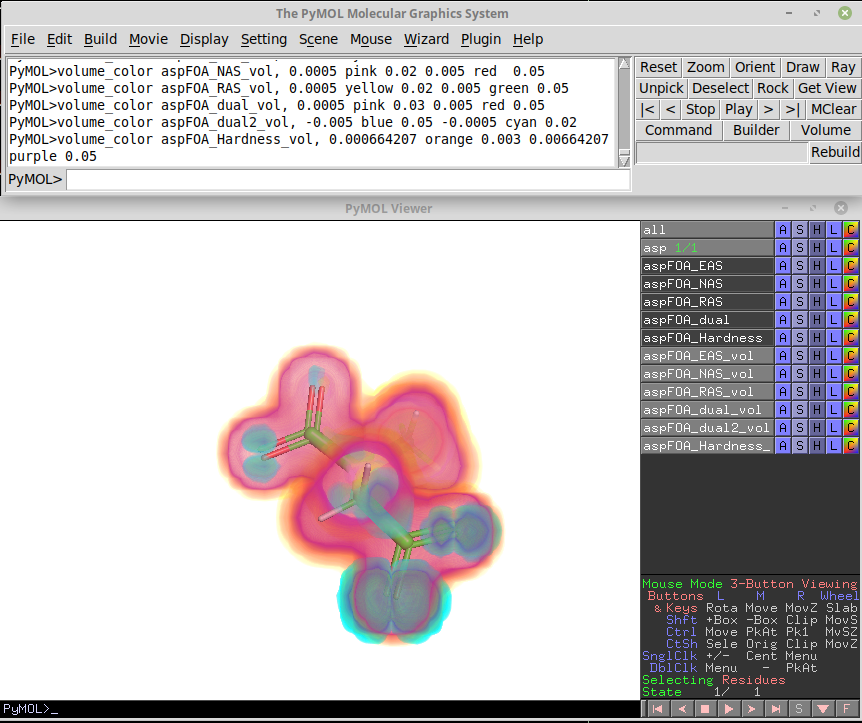
\includegraphics[width=4in]{images/tut4_img9}
			\caption{Descritores locais básicos em representação volumétrica para o ácido aspártico, renderizados no programa Pymol.}
			\label{fig_tut4_7}
		\end{center}
	\end{figure}
\end{minipage}


Na \autoref{fig_tut4_8} o descritor de Netfilicidade, ou as duas fases do descritor dual, é mostrado para o ácido aspártico. Com o comando "Draw", no Pymol é possível renderizar a imagem para salva-lá na resolução desejada e em alta qualidade, resultado na \autoref{fig_tut4_9}. Nessa imagem é possível observar as superfícies renderizadas na cor azul estão localizadas em átomos de oxigênio, e representa a tendência desses locais de receber um ataque eletrolítico, e portanto são nucleófilos, e em rosa e vermelho locais onde tendem a receber um ataque nucleofílico e portanto são eletrófilos. Para o ácido aspártico, quase todos os oxigênios de ácido carboxílico apresentam ser nucleófilos, mas com clara preferência para um dos oxigênios da cadeia lateral. Enquanto isso, no grupo amina apresenta ser um eletrófilo, com uma disposição esférica do descritor ao redor do grupo, sinalizando que qualquer próton pode ser retirado para que o par de elétrons desse nitrogênio carregado positivamente seja restaurado.

\hspace*{-\leftmarginwidth}
\begin{minipage}{\fullwidth}
	\begin{figure}[H]
		\begin{center}
			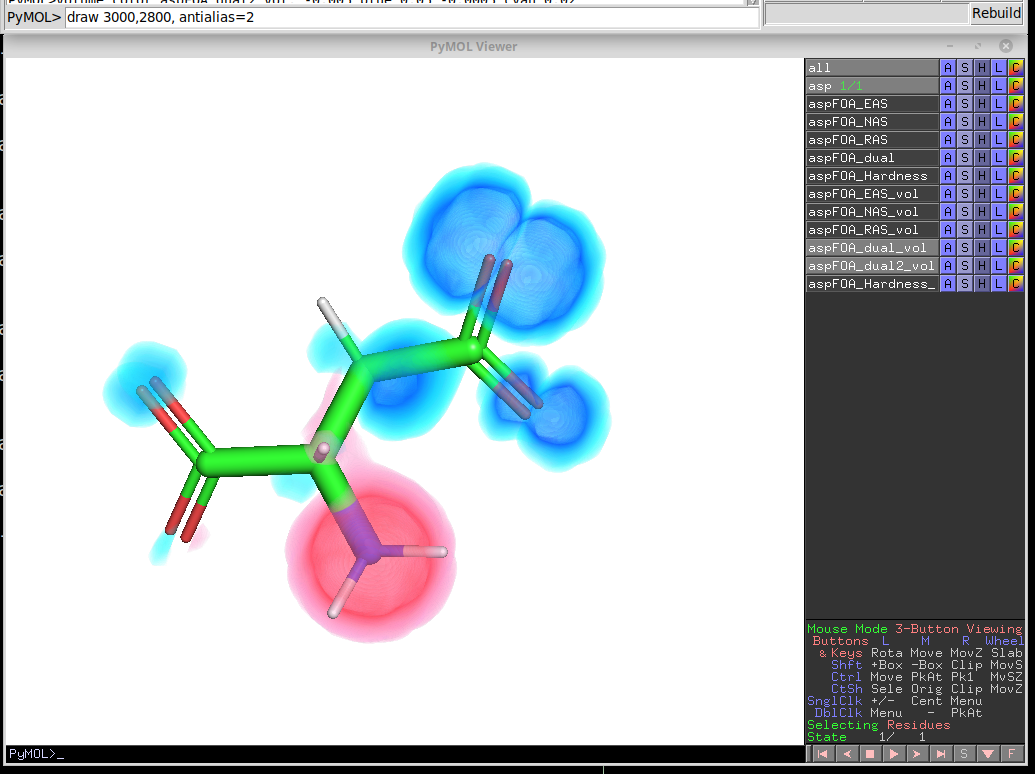
\includegraphics[width=4in]{images/tut4_img10}
			\caption{Descritor de Netfilicidade(dual) mostrado no Pymol para a molécula de ácido aspártico, com o comando no terminal para renderizar a imagem em alta qualidade.}
			\label{fig_tut4_8}
		\end{center}
	\end{figure}
\end{minipage}


\hspace*{-\leftmarginwidth}
\begin{minipage}{\fullwidth}
	\begin{figure}[H]
		\begin{center}
			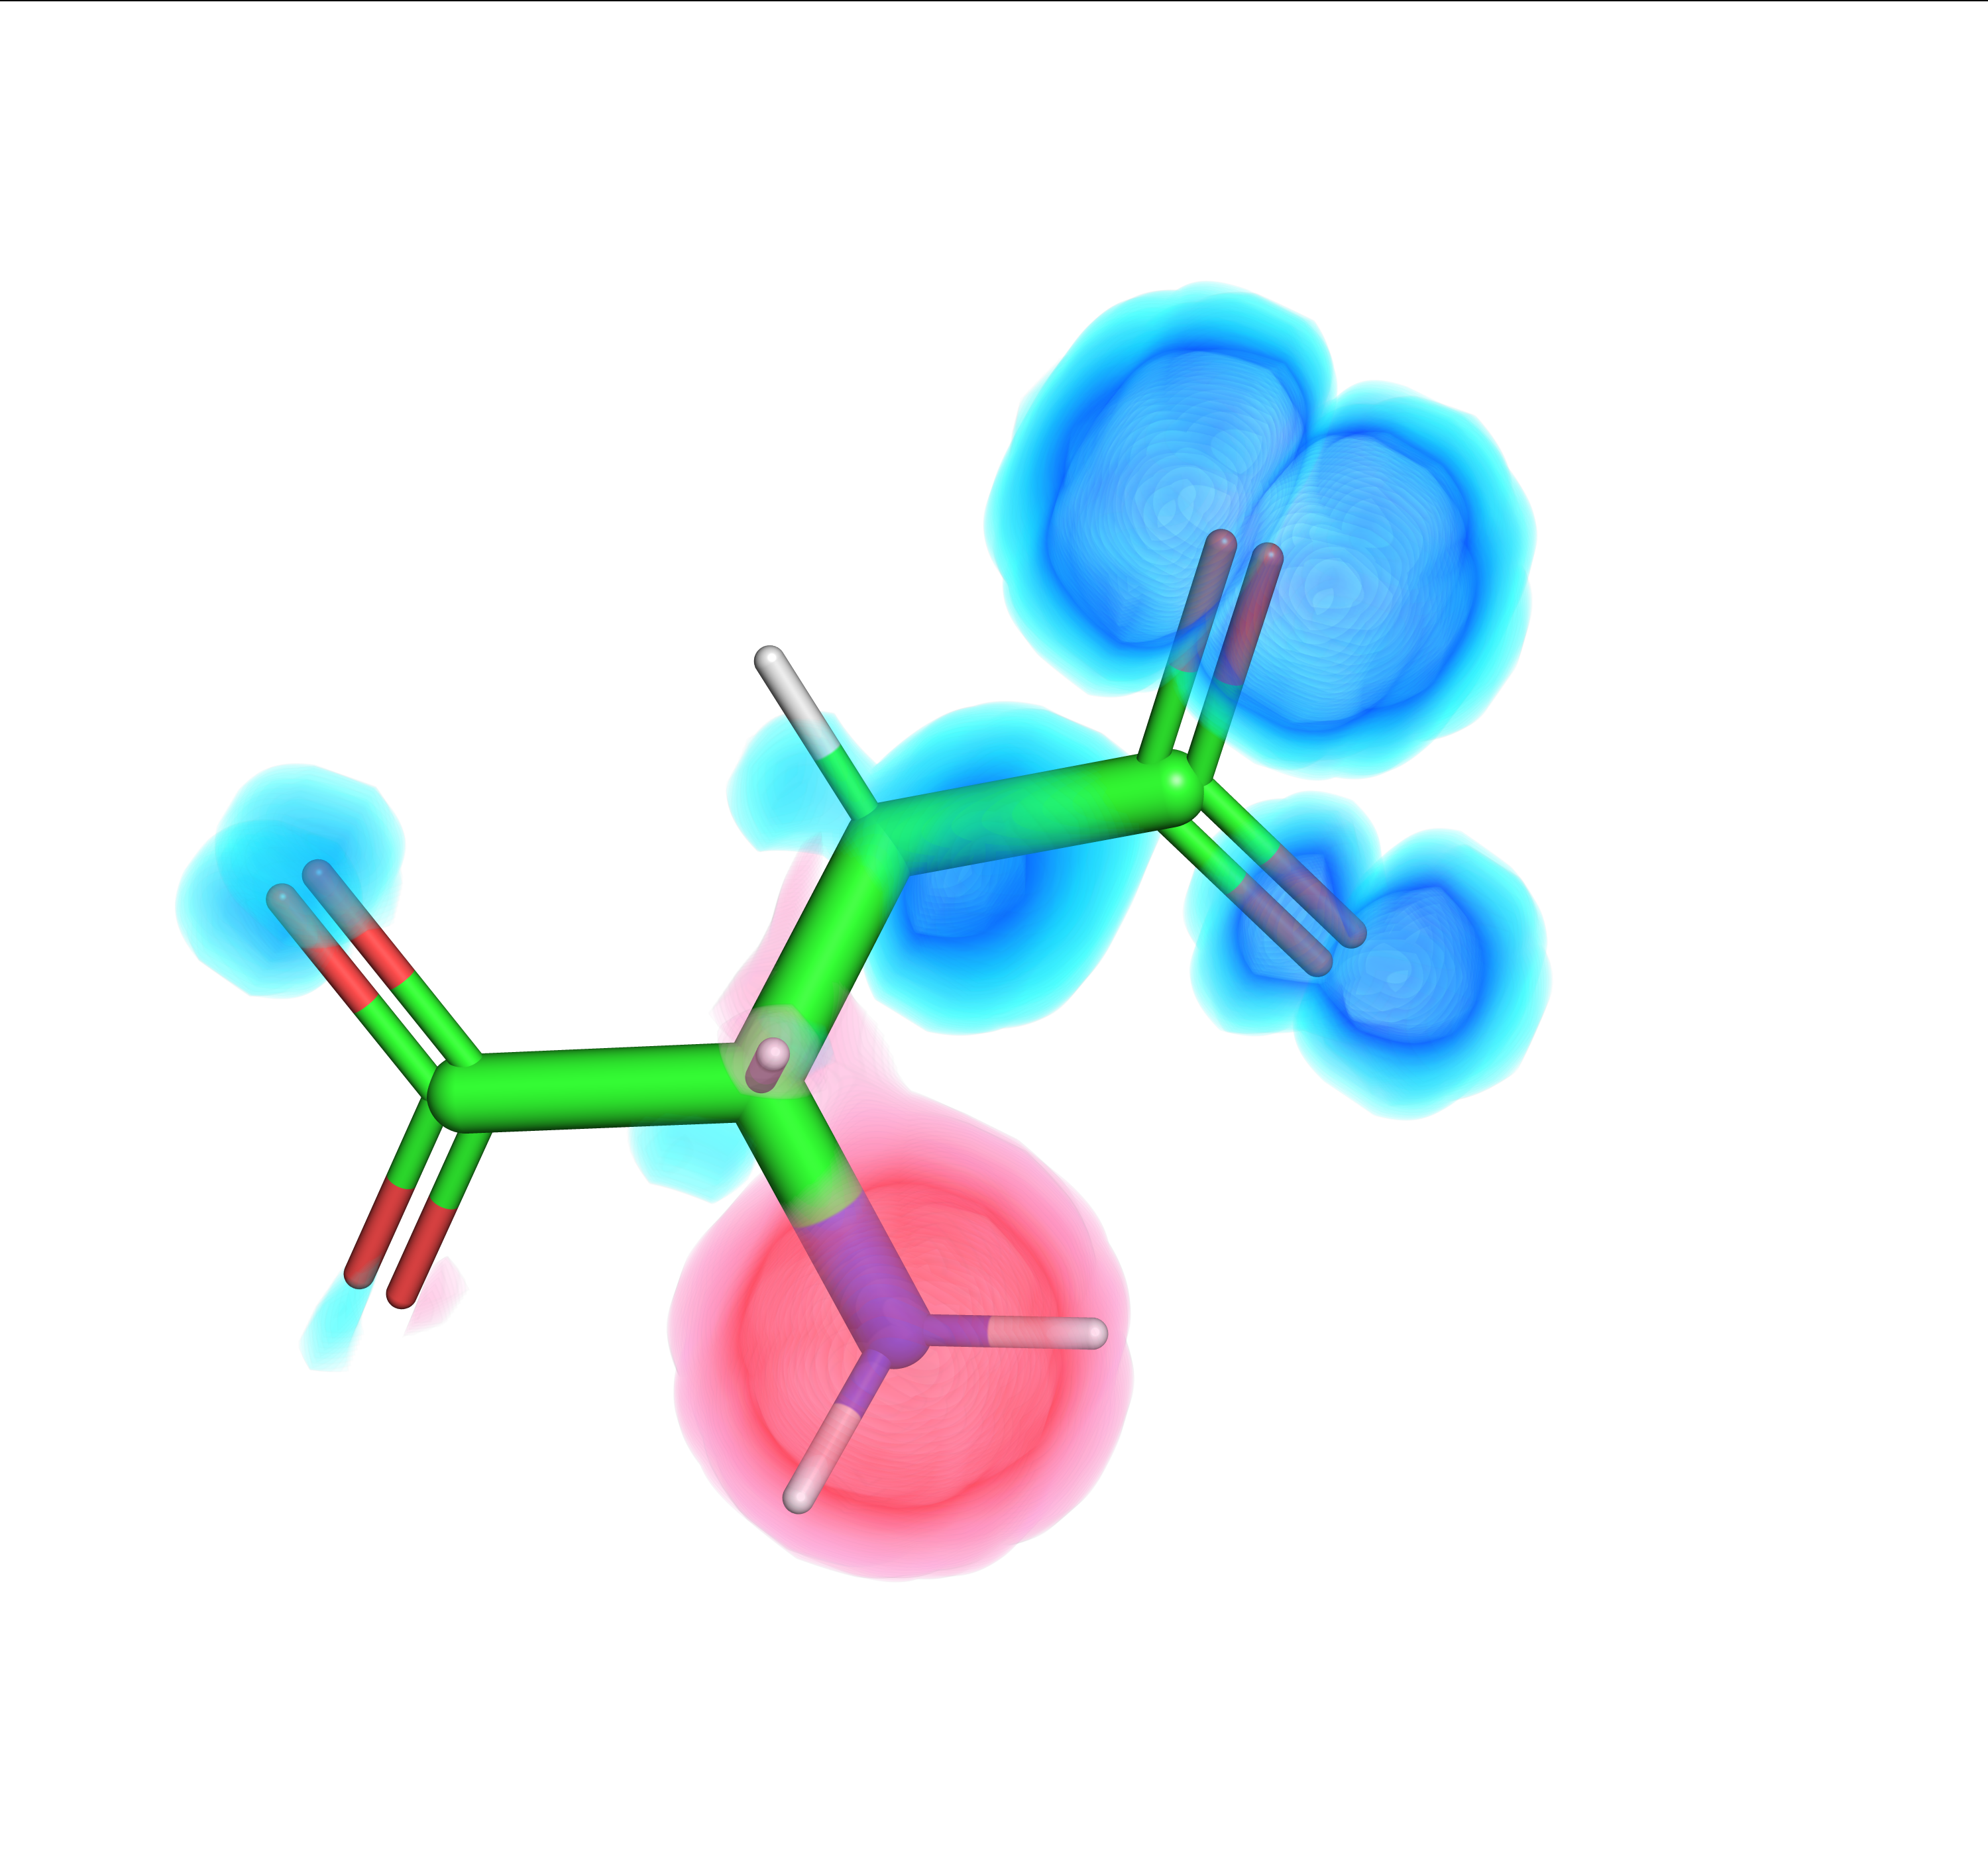
\includegraphics[width=3.5in]{images/tut4_img11}
			\caption{Imagem salve em disco para o descritor de Netfilicidade(dual) para a molécula de ácido aspártico.}
			\label{fig_tut4_9}
		\end{center}
	\end{figure}
\end{minipage}

Passando para a análise do descritor de dureza, é só desativar os objetos de volume anteriores no Pymol e ativamos o último, "aspFOA\_Hardness\_vol", uma representação volumétrica do descritor deve aparecer como mostrado na \autoref{fig_tut4_11}


\hspace*{-\leftmarginwidth}
\begin{minipage}{\fullwidth}
	\begin{figure}[H]
		\begin{center}
			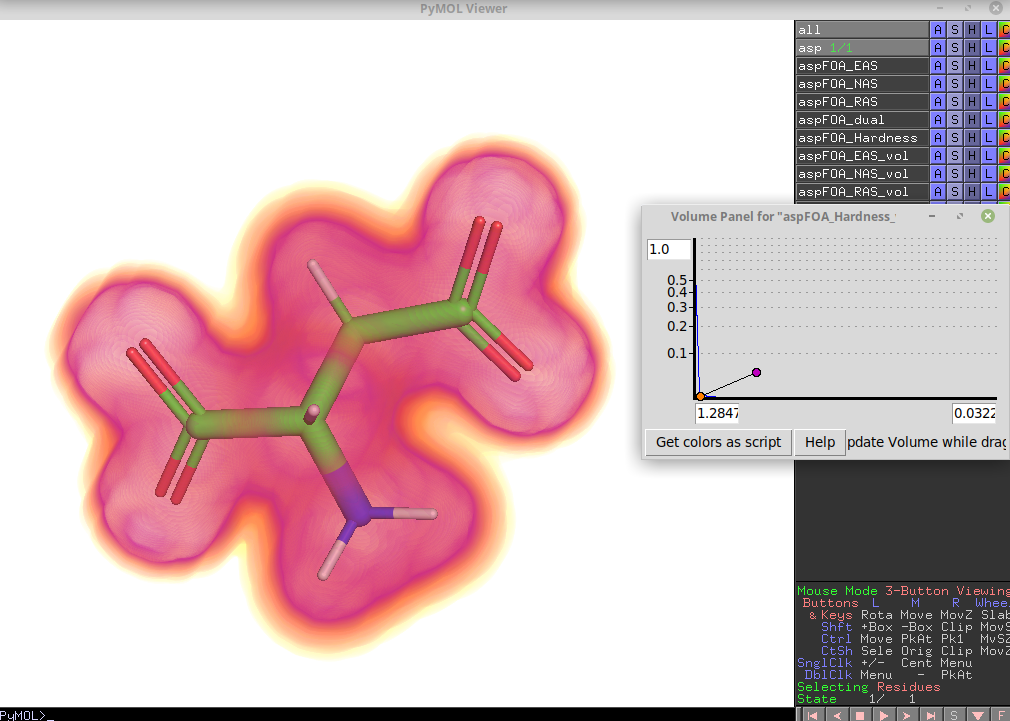
\includegraphics[width=4in]{images/tut4_img13}
			\caption{Descritor de dureza local para o ácido aspártico, mostrando o painel de volume do Pymol onde é possível criar a ajustar as iso-superfícies.}
			\label{fig_tut4_11}
		\end{center}
	\end{figure}
\end{minipage}

A janela que aparece ao lado da \autoref{fig_tut4_12} é aberta colocando em "volume" no painel ao lado da área de execução de comandos do Pymol. Clicando e movimentando os pontos nessa janela é possível mudar as cores, os valores das iso-superfícies e suas opacidades. Também é possível adicionar mais iso-superfícies. Na figura abaixo é mostrado uma modificação feita para o descritores de dureza local. 


\hspace*{-\leftmarginwidth}
\begin{minipage}{\fullwidth}
	\begin{figure}[H]
		\begin{center}
			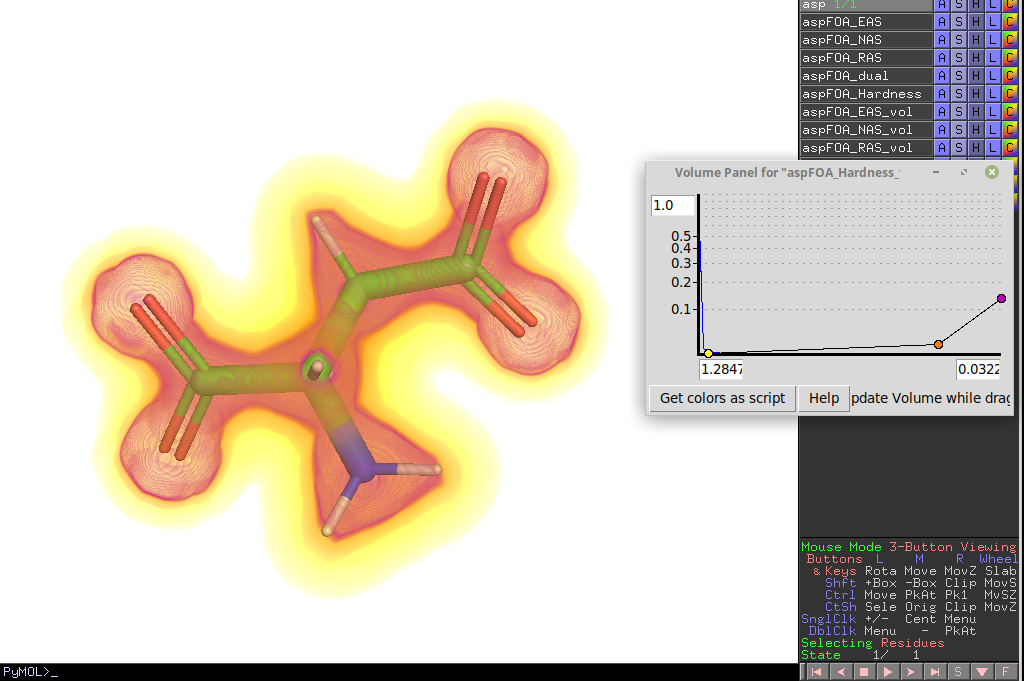
\includegraphics[width=4in]{images/tut4_img14}
			\caption{Descritor de dureza local para o ácido aspártico, mostrando o painel de volume do Pymol com novos valores sugeridos para as iso-superfícies para uma melhor visualização.}
			\label{fig_tut4_12}
		\end{center}
	\end{figure}
\end{minipage}

Repetindo o processo de renderização e de salvar as imagens para os outros sistemas, nós obtemos os descritores para quatro os sistemas, como mostrada nas próximas duas figuras: netfilicidade na \autoref{fig_tut4_13} e de dureza na\autoref{fig_tut4_14}.

\hspace*{-\leftmarginwidth}
\begin{minipage}{\fullwidth}
	\begin{figure}[H]
		\begin{center}
			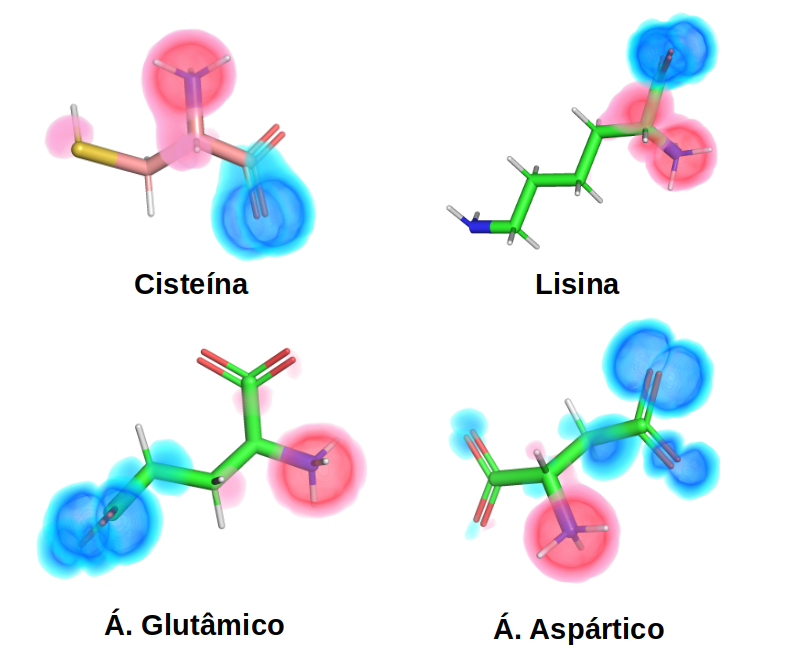
\includegraphics[width=5in]{images/tut4_img15}
			\caption{Descritor local de Netfilicidade para os quatro amino-ácidos analisados no tutorial.}
			\label{fig_tut4_13}
		\end{center}
	\end{figure}
\end{minipage}

\hspace*{-\leftmarginwidth}
\begin{minipage}{\fullwidth}
	\begin{figure}[H]
		\begin{center}
			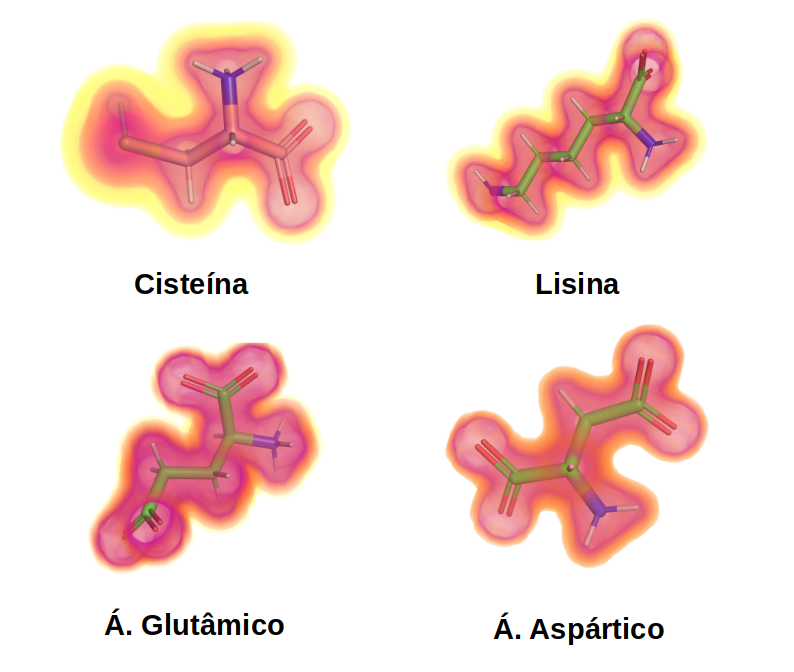
\includegraphics[width=5in]{images/tut4_img16}
			\caption{Descritor de dureza local para os quatro amino-ácidos analisados no tutorial, usando o método de potencial químico local.}
			\label{fig_tut4_14}
		\end{center}
	\end{figure}
\end{minipage}

\hspace*{-\leftmarginwidth}
\begin{minipage}{\fullwidth}
	\begin{figure}[H]
		\begin{center}
			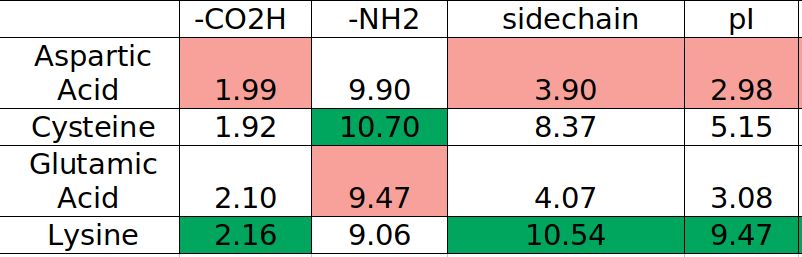
\includegraphics[width=5in]{images/tut4_img17}
			\caption{Tabela com os resultados de descritores locais para os grupos aceptores/doadores de prótons da cadeia principal de cada um dos quatro amino-ácidos.}
			\label{fig_tut4_15}
		\end{center}
	\end{figure}
\end{minipage}

\hspace*{-\leftmarginwidth}
\begin{minipage}{\fullwidth}
	\begin{figure}[H]
		\begin{center}
			\includegraphics[width=4in]{images/tut4_img18}
			\caption{Tabela com os resultados de descritores locais para os átomos aceptores/doadores de prótons da cadeia lateral de cada um dos quatro amino-ácidos. Também uma tabela complementar com os descritores globais, cargas parciais e o valor conhecido de Potencial de Ionização.}
			\label{fig_tut4_16}
		\end{center}
	\end{figure}
\end{minipage}

Juntando as informações que podemos observar dos descritores condensados e volumétricos que essas quantidades teóricas conseguem localizar os as porções das moléculas onde transferências de prótons são mais prováveis de ocorrer. O descritores de dureza química é o mais apropriado para esse tipo de processo, transferência de pequenos grupos carregados, e mostrou uma relação com o pKa dos grupos amina, com a cisteína mostrando a maior dureza no nitrogênio e também o maior pKa. Obviamente, esse pequeno estudo está repleto de limitações e só tem intenção de mostrar uma relação prática dos resultados obtidos com o PRIMoRDiA e um problema de modelagem molecular comum.

\newpage
\section{Tutorial 5: Análise de Reação Enzimática}

Nesse tutorial vai ser trabalho um exemplo prático de como o PRIMoRDiA pode ser explorado para o estudo de sistemas biológicos e seus principais processos. A grande força do PRIMoRDiA está nos descritores modificados para macromoléculas que disponibiliza e na automatização do processamento dessas propriedades eletrônicas. Vamos entrar com a estrutura eletrônica de um fragmento de uma sistema enzimático para uma pequena trajetória de reação e sairemos com um resumo estatístico da evolução dos descritores nesse processo.


\subsection{Contextualização}

Reações enzimáticas são reações químicas catalisadas por proteínas, que fazem com que transformações químicas ocorram em um tempo hábil para o funcionamento do metabolismo de organismos vivos. Portanto, as enzimas são componentes importantíssimos para a manutenção da vida, participando desde a replicação de DNA até a decomposição do açúcar.

O estudo do mecanismo dessas reações é muito importante para o desenvolvimento de drogas, entendimento de metabolismo, mecanismos de doenças e replicação de micro-organismos e aplicações industriais dessas enzimas. Em um dos estudos do nosso grupo, foi com o mecanismo da reação catalisada pela triose-fosfato-isomerase (TIM), mais especificamente a etapa mostrada no esquema abaixo

Nós utilizamos esse enzima para testar a eficácia dos descritores de caracterizar teoricamente essa reação, descrevendo as principais forças, interações e efeitos do ambiente. A TIM é uma das enzimas mais caracterizadas na literatura, é uma enzima central no caminho glicolítico da interconversão do 3-fosfato D-gliceroldeído (GAP em inglês) para o fosfato dihidroxiacetona, com grande eficiência.

Nesse tutorial nós vamos calcular os descritores para esse sistema em uma trajetória de reação obtida por simulação de QM/MM.

\hspace*{-\leftmarginwidth}
\begin{minipage}{\fullwidth}
	\begin{figure}[H]
		\begin{center}
			\includegraphics[width=3.5in]{images/tut6_img0}
			\caption{Representação do mecanismo de catálise enzimática estudado nesse tutorial.}
			\label{fig_tut6_0}
		\end{center}
	\end{figure}
\end{minipage}

\subsection{Arquivos necessários e Execução}

Os arquivos necessários para os cálculos desse tutorial estão na pasta . São arquivos de ".aux" e ".pdb", para as etapas do caminho de reação. Esse caminho de reação engloba somente 110 átomos, feito dessa forma para obter arquivos mais leves para o tutorial. A trajetória do scan foi obtida como explicado no tutorial do easyhybrid.

Para fazer as análises especiais para a reação enzimática nós vamos outro método de execução, que é sinalizado no PRIMoRDiA pela keyword "reaction" depois de "\#RT" na primeira linha, ou seja, o Run Type passa para o modo de reação. Na pasta já tem o arquivo de input, que agora possui vários elementos importantes de citar, e está mostrado na figura abaixo

É possível perceber que tem varias outras linhas com keywords antes não usadas e somente uma entrada de arquivo ".aux" para rodar com a opção 3 de cálculo. Como esse é um cálculo para reação química, o PRIMoRDiA entende aquela entrada como valendo para todos os auxs na pasta que tenham o sufixo sinalizado, nesse caso no nosso input foi o sufixo "sys", rodando de "sys0.aux" até "sys14.aux", obedecendo o parâmetro "dimX".

Vamos analisar os outros parâmetros do input

\hspace*{-\leftmarginwidth}
\begin{minipage}{\fullwidth}
\begin{lstlisting}[caption={Input editado para execução do tutorial 3},label={tut402}]
#RT reaction 
#PR eband 2 Rscript pymols
#Reaction RC1 98 107 51
#Reaction dimX 15
#TRJ residues 2 4 7
3 sys.aux none 30 10 sys.pdb mopac  0 0 0 0 EW
\end{lstlisting}
\end{minipage}

Segunda linha
\begin{itemize}
	\item Segunda linha
	\begin{itemize}
	\item \#PR:     flag para sinalizar que serão dados parâmetros para o PRIMoRDiA
	\item eband:   keyword sinalizando que o próxima parâmetro é um inteiro com o valor de energia de corte para considerar os orbitais moleculares
	\item Rscript: Keyword importante par gerar os scripts de análise dos descritores durante a trajetória de reação
	\item pymols:  keyword para o output de scripts para o Pymol
	\end{itemize}
	\item Terceira linha
	\begin{itemize}
	\item \#Reaction: flag para sinalizar que vai ser passado parâmetros para análise de coordenada de reação
	\item RC1: keyword sinalizando que vais ser passado o número dos átomos que compõem a coordenada de reação
	\item 98: número do átomo de carbono (C1) do GAP 
	\item 107:número do átomo de hidrogênio (H1) ligado ao DHAP
	\item 51: número do átomo de oxigênio (OE2) do GLU
	\end{itemize}
	\item Quarta Linha
	\begin{itemize}
	\item \#Reaction: flag para sinalizar que vai ser passado parâmetros para análise de coordenada de reação
	\item dimX     : keyword para sinalizar que o próximo valor na linha da o número de etapas da trajetória
	\item 15       : número de etapas da trajetória
	\end{itemize}
	\item Quinta Linha 
	\begin{itemize}
	\item \#Reaction: flag para sinalizar que vai ser passado parâmetros para análise de coordenada de reação
	\item dimX      : keyword para sinalizar que o próximo valor na linha da o número de etapas da trajetória
	\item 15        : número de etapas da trajetória
	\end{itemize}
	\item Sexta Linha 
	\begin{itemize}
	\item 3      : opção de cálculo do PRIMoRDiA para macromoléculas
	\item sys.aux: nome base para os arquivos, antes do ponto o prefixo sem o número que indica o frame, e depois do ponto a extensão do arquivo
	\item none   : keyword sinalizando que nenhum métodos de dureza local foi pedido para cálculo da representação volumétrica, o que já não seria feito já que o valor de grid é zero
	\item 0      : finura do grid para representação volumétrica, sempre deixar em zero até uma nova atualização do software
	\item 10     : número máximo de orbitais moleculares de fronteira para ser utilizado se o método de combinação de orbitais for BD
	\item sys.pdb: nome base para os arquivos de pdb, mesma lógica para os arquivos que contém a estrutura eletrónica
	\item mopac  : nome do programa de onde foi calculada a estrutura eletrónica
	\item 0      : parâmetro não relevante com grid 0
	\item 0      : parâmetro não relevante com grid 0
	\item 0      : parâmetro não relevante com grid 0
	\item 0      : parâmetro não relevante com grid 0
	\item EW     : Keyword para o método de combinação de orbitais moleculares
	\end{itemize}
\end{itemize}

\subsection{Análise dos Resultados}

Para analisar todos os descritores e outras propriedades de energia, o PRIMoRDiA cria um script para executar no R para gerar automaticamente gráficos dessas quantidades variando em função das etapas. Depois da execução deve aparecer arquivos com sufixo ".R", um deles com nome "sys0\_reaction\_analysis.R" e outro "sys0\_residuos\_analysis.R". Vamos executar o primeiro com o Rscript, como no comando abaixo


Depois desse comando, o R deve produzir diversos arquivos de imagem com propriedades globais e locais para cada átomo da coordenada de reação. Na figura abaixo é mostrado um desses arquivos com as propriedades globais

No primeiro gráfico da figura acima HOF é o calor de formação  (heat of formation) que o Mopac calcula, e é uma das melhores formas de variação de energia em uma reação química simulada com método semiempírico. Lembrando que todas essas propriedades são em referência ao primeiro valor, ou seja, cada ponto uma variação ao estado inicial. Nessas simulações uma estrutura que normalmente se deseja determinar é a estrutura de transição, que é determinada pelo ponto máximo de variação de energia, nesse caso na penúltima etapa. No entanto, nesse nosso calculo com PM6, a área quântica foi bem menor do que a utilizada no na nossa publicação e o HOF não foi um bom indicador do estado de transição. Já a energia eletrônica mostra um primeiro máximo no ponto zero da coordenada de reação, que é o momento que o próton está a mesma distância do carbono e do oxigênio. Em geral, os outros descritores globais indicam um aumento da moleza química (softness) e consequente diminuição da dureza (hardness), aumento do potencial químico e da eletrofilicidade total indicam que o sistema tende a receber transferência de elétrons.

Na figura a baixo podemos conferir a variação de energia para mesma reação calculada com diversos métodos, publicado em um artigo na Journal of Chemical Information Modeling 

\hspace*{-\leftmarginwidth}
\begin{minipage}{\fullwidth}
	\begin{figure}[H]
		\begin{center}
			\includegraphics[width=4in]{images/tut6_img2}
			\caption{.}
			\label{fig_tut6_1}
		\end{center}
	\end{figure}
\end{minipage}

Na análise que foi publicada, boa parte dos métodos apresenta um estado de transição perto de -0.025 da coordenada de reação, quase no ponto de igual distância da transferência do próton, depois há uma vale, denotando um estado intermediário e depois mais um aumento de energia até outro vale no qual o produto deve se acomodar. Como visto na imagem acima, o PM6 é o método mais discordante em relação ao calor de formação. Na figura seguinte, nós mostramos os descritores para o átomo de oxigênio do resíduo GLU. No script gerado pelo PRIMoRDiA nós analisamos 9 propriedade por átomo da coordenada de reação. Para o oxigênio é interessante ressaltar algumas, como o decréscimo na densidade eletrônica, atingindo um mínimo no estado de transição e depois retomando o valor nos produtos. A carga parcial aumenta também, indicando que há uma transferência de elétrons do oxigênio para o carbono, e que depois o o sistema em volta faz uma "devolução" de carga para o oxigênio, mas que no final ainda fica com menos, já que agora o grupo carboxilico que pertence está protonado e portanto neutro. Já para a dureza local esse átomo apresenta comportamentos diferentes para cada tipo de método de cálculo, para interpretar o que cada um significa é importante entender cada modelo. Brevemente, a dureza baseada no LCP tem mais correção com o descritor global de dureza, indicando que esse tinha a propensão de interagir por processo duro-duro e depois foi diminuindo esse comportamento conforme foi transferindo carga. 


\hspace*{-\leftmarginwidth}
\begin{minipage}{\fullwidth}
	\begin{figure}[H]
		\begin{center}
			\includegraphics[width=4in]{images/tut6_img3}
			\caption{.}
			\label{fig_tut6_2}
		\end{center}
	\end{figure}
\end{minipage}

Os descritores para o carbono C1 estão na próxima figura. Tem bastante coisa interessante para analisar nesse caso. Primeiro, é interessante como para dois métodos de dureza o valor máximo condiz com o estado de transição e perfila muito bem a reação. Já que a interação dominante para transferência de prótons é a duro-duro, o carbono assume o valor máximo para esse descritor, em dois métodos mepEE e LCP. O método de dureza baseado no potencial de Fukui da a força exercida nos núcleos em respeito da varição do número de elétrons, o que ten una interpretação mais diferente da geral sobre dureza comum. 

\hspace*{-\leftmarginwidth}
\begin{minipage}{\fullwidth}
	\begin{figure}[H]
		\begin{center}
			\includegraphics[width=4in]{images/tut6_img4}
			\caption{.}
			\label{fig_tut6_3}
		\end{center}
	\end{figure}
\end{minipage}

Os descritores para o átomo transferido, o hidrogênio do DHAP (H1), se encontra na figura de baixo. Os descritores baseados nos orbitais moleculares, como electrophilicidade, nucleofilicidade e netfilicidade mostraram variação mas com valores muito baixos. Agora é interessante como a densidade eletrônica vai diminuindo, se tornando cada vez mais um próton, um hidrogênio carregado positivamente. A dureza local com maior ligação com as interações eletrostáticas ( MEP EE ), foi a que apresentou maior coerência com o processo, com um aumento das interações eletrostáticas pŕoximo ao estado de transição, diminui e atinge o máximo nos produtos, onde a carga parcial atinge o máximo, sendo que esse átomo tende a ser transferido pelo mesmo tipo de interação.

Como no Tutorial 3, vamos gerar imagens do descritores para alguns pontos da trajetória. O PRiMoRDiA escreve para cada arquivo um script de Pymol para automatizar a visualização dos descritores. Abra o Pymol e execute o arquivo com o prefixo "sys0" e sufixo ".pym", como na figura abaixo. 

\hspace*{-\leftmarginwidth}
\begin{minipage}{\fullwidth}
	\begin{figure}[H]
		\begin{center}
			\includegraphics[width=4in]{images/tut6_img5}
			\caption{.}
			\label{fig_tut6_4}
		\end{center}
	\end{figure}
\end{minipage}

Na figura abaixo o descritor de susceptibilidade de ataque eletrofílico (EAS), e um comando para carregar um PDB que já tinha na pasta, 7TIM.pdb, que contém o toda a proteína.

\hspace*{-\leftmarginwidth}
\begin{minipage}{\fullwidth}
	\begin{figure}[H]
		\begin{center}
			\includegraphics[width=4in]{images/tut6_img6}
			\caption{.}
			\label{fig_tut6_5}
		\end{center}
	\end{figure}
\end{minipage}

As pŕoximas figuras foram resultado do processo de renderização no pymol para o descritor de dureza local com o segundo método disponível no PRIMoRDiA. O objeto com a proteína inteira foi colorido com os carbonos em verde e escondido todas as outras representação que não fossem cartoon para não atrapalhar a visualização do objeto com o descritor. Para a paleta escolhida o comando utilizado foi 

` spectrum b, white_yellow_orange_red_black, minimum=0.1,maximum=0.2 `

Esses valores podem sofrer pequenos ajustar para melhorar o destaque dos átomo com o maior valor de dureza. Depois, com o comando "ray" seguido do "png" as imagens foram salvas. 


\hspace*{-\leftmarginwidth}
\begin{minipage}{\fullwidth}
	\begin{figure}[H]
		\begin{center}
			\includegraphics[width=4in]{images/tut6_img8}
			\caption{.}
			\label{fig_tut6_7}
		\end{center}
	\end{figure}
\end{minipage}

A imagem abaixo é a dureza local para a primeira etapa da coordenada


\hspace*{-\leftmarginwidth}
\begin{minipage}{\fullwidth}
	\begin{figure}[H]
		\begin{center}
			\includegraphics[width=4in]{images/tut6_img9}
			\caption{.}
			\label{fig_tut6_8}
		\end{center}
	\end{figure}
\end{minipage}

A imagem abaixo é a dureza local para a sétima etapa da coordenada

\hspace*{-\leftmarginwidth}
\begin{minipage}{\fullwidth}
	\begin{figure}[H]
		\begin{center}
			\includegraphics[width=4in]{images/tut6_img10}
			\caption{.}
			\label{fig_tut6_9}
		\end{center}
	\end{figure}
\end{minipage}

A imagem abaixo é a dureza local para a última etapa da coordenada


\hspace*{-\leftmarginwidth}
\begin{minipage}{\fullwidth}
	\begin{figure}[H]
		\begin{center}
			\includegraphics[width=4in]{images/tut6_img11}
			\caption{.}
			\label{fig_tut6_10}
		\end{center}
	\end{figure}
\end{minipage}

O PRIMoRDiA também escreve scripts especiais do R para a análise dos descritores para residos específicos, indicados no input, produzindo gráficos de barra com a média e o desvio padrão, como na figura abaixo para o descritor de eletrofilicidade, o mesmo que o NAS.

\hspace*{-\leftmarginwidth}
\begin{minipage}{\fullwidth}
	\begin{figure}[H]
		\begin{center}
			\includegraphics[width=3in]{images/tut6_img12}
			\caption{.}
			\label{fig_tut6_11}
		\end{center}
	\end{figure}
\end{minipage}

E na próxima figura para a nucleofilicidade, ou descritor EAS

\hspace*{-\leftmarginwidth}
\begin{minipage}{\fullwidth}
	\begin{figure}[H]
		\begin{center}
			\includegraphics[width=3in]{images/tut6_img13}
			\caption{.}
			\label{fig_tut6_12}
		\end{center}
	\end{figure}
\end{minipage}


Também, é acompanhado a variação desses valores durante a trajetória com o cálculo de médias móveis, como na figura abaixo é mostrado para densidade eletrônica em cada resido 

\hspace*{-\leftmarginwidth}
\begin{minipage}{\fullwidth}
	\begin{figure}[H]
		\begin{center}
			\includegraphics[width=3in]{images/tut6_img14}
			\caption{.}
			\label{fig_tut6_13}
		\end{center}
	\end{figure}
\end{minipage}

Na figura abaixo é mostrado para o primeiro método de dureza local 

\hspace*{-\leftmarginwidth}
\begin{minipage}{\fullwidth}
	\begin{figure}[H]
		\begin{center}
			\includegraphics[width=3in]{images/tut6_img15}
			\caption{.}
			\label{fig_tut6_14}
		\end{center}
	\end{figure}
\end{minipage}

E em seguida as médias móveis para moleza local

\hspace*{-\leftmarginwidth}
\begin{minipage}{\fullwidth}
	\begin{figure}[H]
		\begin{center}
			\includegraphics[width=3in]{images/tut6_img16}
			\caption{.}
			\label{fig_tut6_15}
		\end{center}
	\end{figure}
\end{minipage}

Podemos ver como a densidade eletrônica e a moleza local no LIG, o substrato, aumenta. Nessa estrutura de transição formada no produto da nossa simulação, o substrato forma uma ligação dupla quando o próton é doado, e como os descritores indicam o carbono e a moléculas receberam doação de carga. O aumento da moleza pode significar que agora com a dupla formada essa molécula tem maior propensão de formar ligações covalentes através de sobreposição de orbitais moleculares e também transferir carga. 

Há diversas análises que podemos fazer baseados nos descritores de reatividade, que por sua vez também são numerosos, para cada átomo envolvido e para cada resíduo. O PRIMoRDiA fornece uma forma automática de dispor todos esses resultados da forma mais pronta para análise possível. 


\end{document}